\documentclass{article}
\usepackage[utf8]{inputenc}

\title{Laboratorio03_INTELIGENCIA_NEGOCIOS}
\author{edwartbalcon}
\date{Septiembre 2021}

\usepackage[utf8]{inputenc}
\usepackage[spanish]{babel}
\usepackage{natbib}
\usepackage{graphicx}

\begin{document}

\title{Caratula}

\begin{titlepage}
\begin{center}
\begin{Large}
\textbf{UNIVERSIDAD PRIVADA DE TACNA} \\
\end{Large}
\vspace*{-0.025in}
\begin{figure}[htb]
\begin{center}

\includegraphics[width=6cm]{./images/logo_UPT}
\end{center}
\end{figure}
\vspace*{-0.025in}
\begin{Large}
\textbf{FACULTAD DE INGENIERIA} \\
\end{Large}
\vspace*{0.05in}
\begin{Large}
\textbf{Escuela Profesional de Ingeniería de Sistema} \\
\end{Large}


\vspace*{0.4in}

\vspace*{0.1in}
\begin{Large}
\textbf{Informe de laboratorio 03: Creando un Reporte Interactivo en Power BI} \\
\end{Large}

\vspace*{0.3in}
\begin{Large}
\textbf{Curso: Inteligencia de negocios} \\
\end{Large}

\vspace*{0.3in}
\begin{Large}
\textbf{DOCENTE: Ing. Patrick Cuadros Quiroga} \\
\end{Large}

\vspace*{0.2in}
\vspace*{0.1in}
\begin{large}

\begin{Large}
\textbf{Alumno: Balcon Coahila, Edwart Juan\hfill	(2013046516) } \\
\end{Large}

\vspace*{0.15in}
\begin{Large}
\textbf{Tacna – Perú} \\
\end{Large}

\vspace*{0.05in}
\begin{Large}
\textbf{2021 } \\
\end{Large}

\end{large}
\end{center}

\end{titlepage}


\newpage

\section{Conexión a datos de Power BI}

\textbf{1.1. Abrir SQL Server Management Studio, y conectar a la instancia de base de
 datos \textbf{(local)} utilizando autenticación de Windows.}

    \begin{center}
		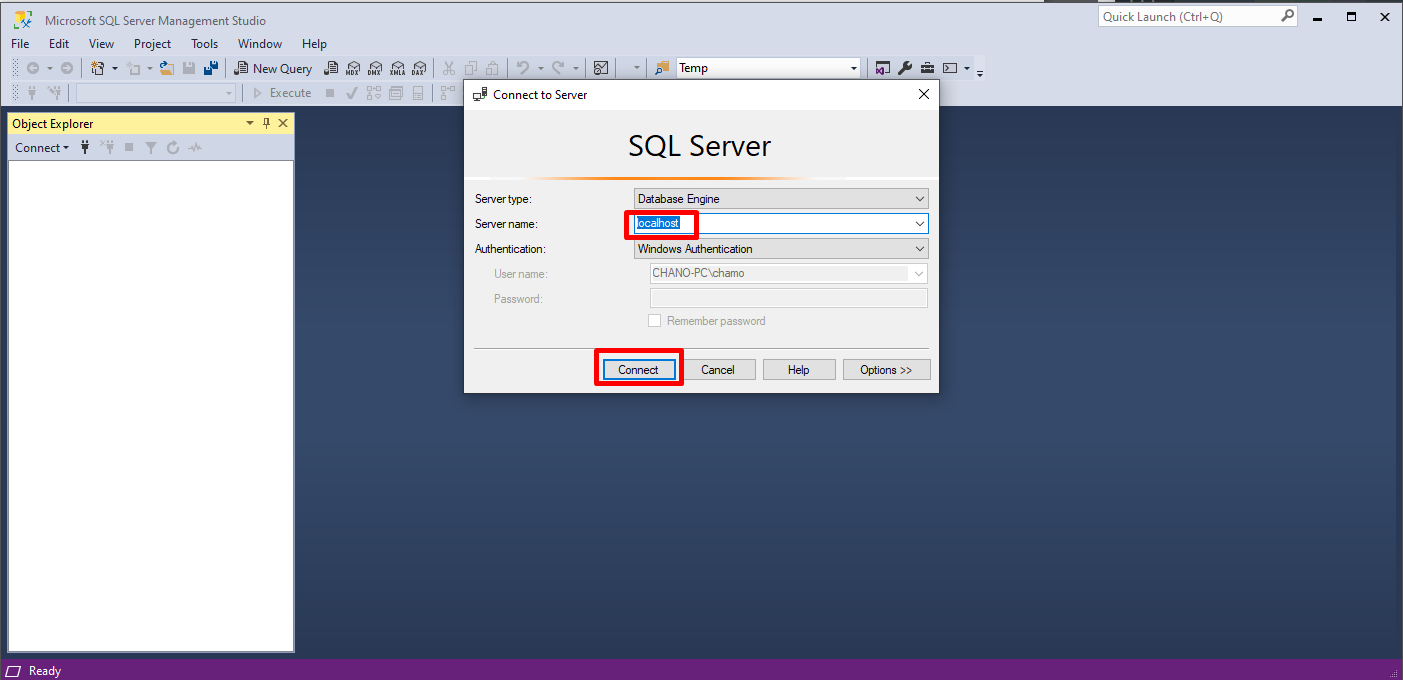
\includegraphics[width=14cm]{./images/1} 
	\end{center}

\textbf{1.2. En el menú Archivo \textbf{(File)}, en el submenu Abrir \textbf{(Open)}, hacer 
click en \textbf{Project/Solution}, y buscar el archivo \textbf{Project.ssmssln}.}

    \begin{center}
		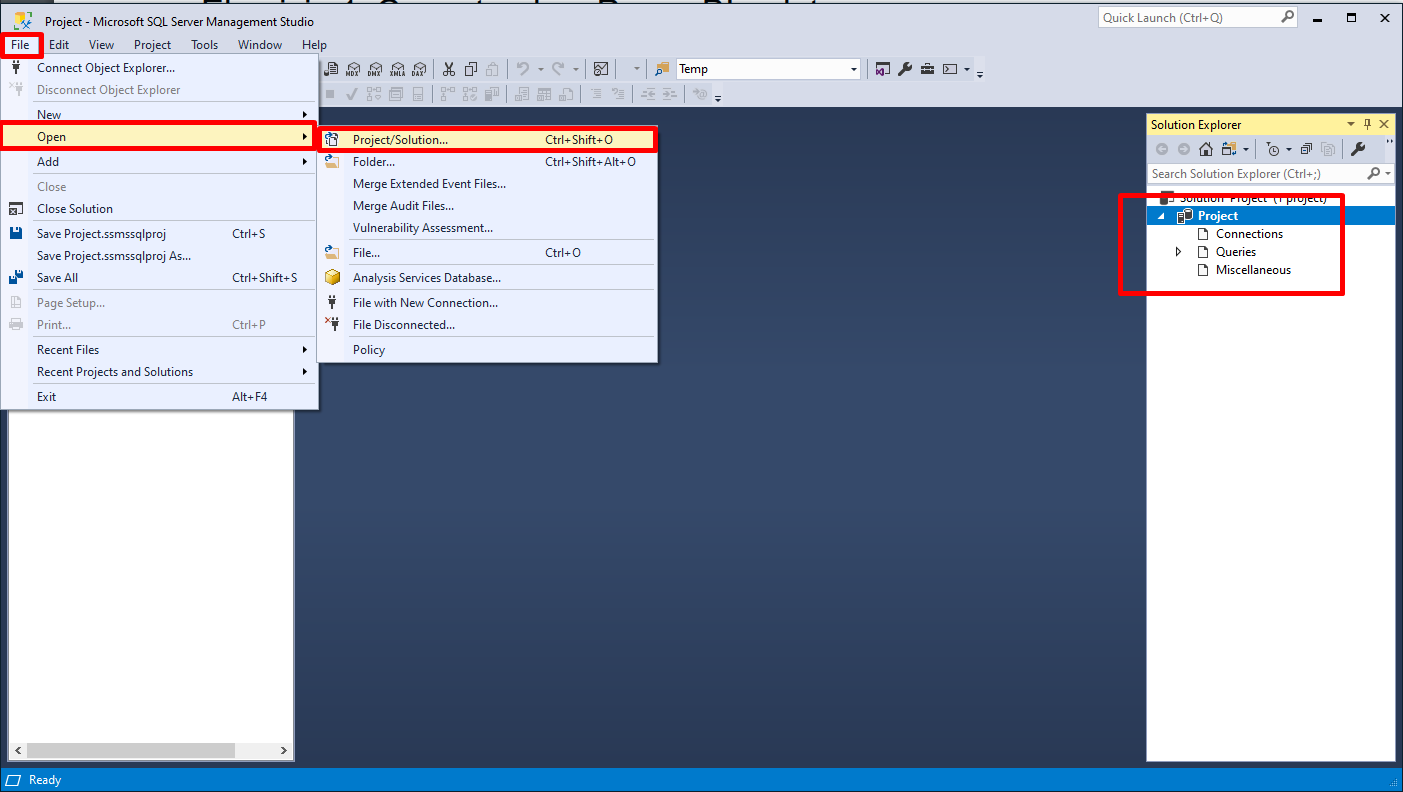
\includegraphics[width=14cm]{./images/2} 
	\end{center}

\textbf{1.3. En el Explorador de Soluciones, expandir Consultas \textbf{(Queries)}, y luego 
hacer doble click en el archivo \textbf{Lab Exercise 1.sql}.}

    \begin{center}
		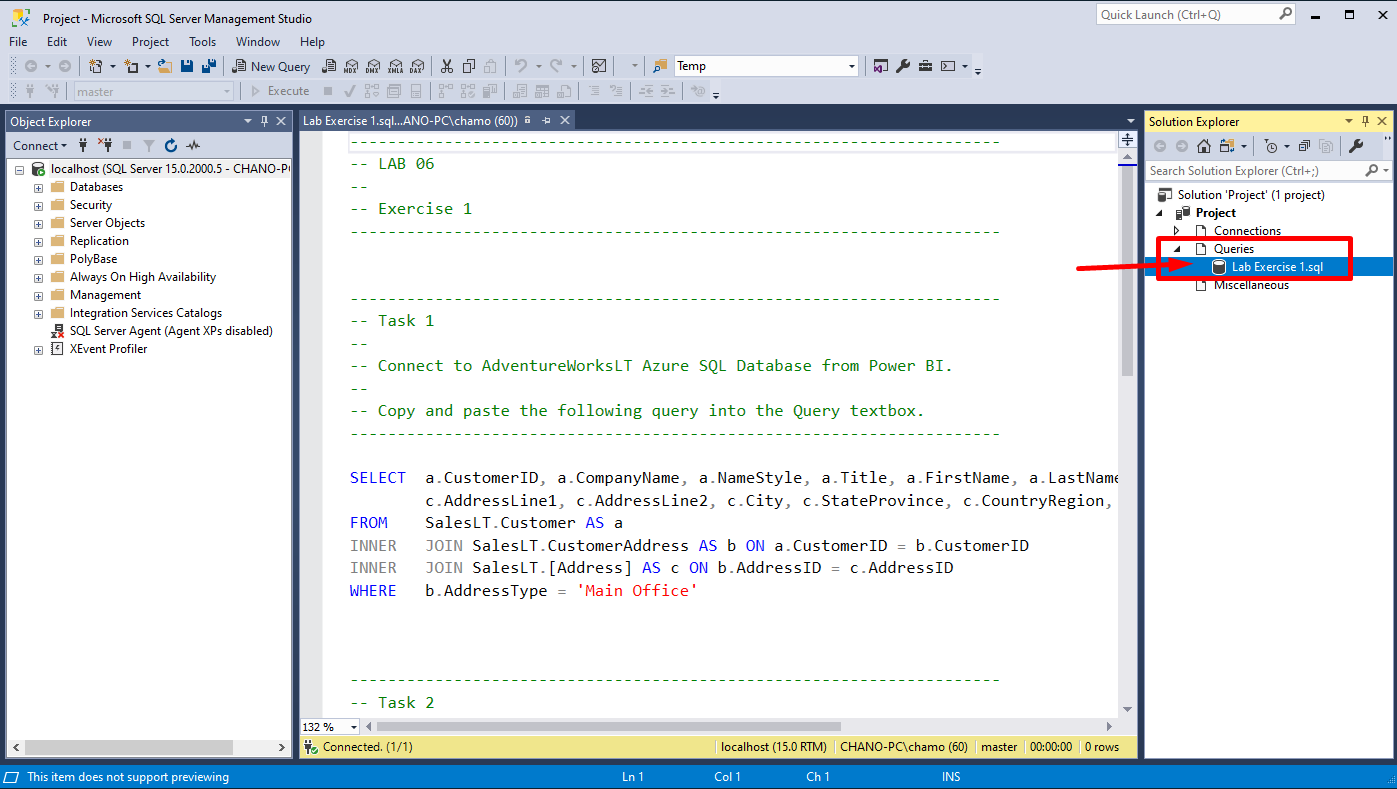
\includegraphics[width=14cm]{./images/3} 
	\end{center}

\textbf{1.4. Abrir \textbf{Power BI Desktop}.}

    \begin{center}
		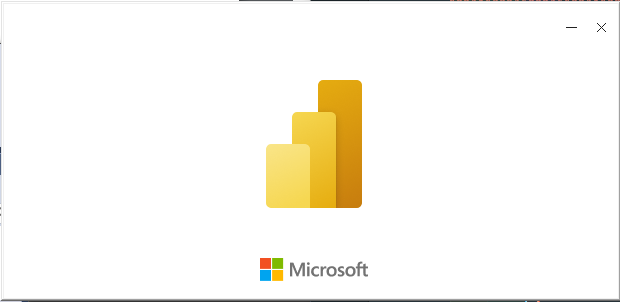
\includegraphics[width=14cm]{./images/4} 
	\end{center}
	
\newpage
\textbf{1.5.En la ventana Power BI Desktop, hacer click en Obtener Data \textbf{(Get Data)}.}

    \begin{center}
		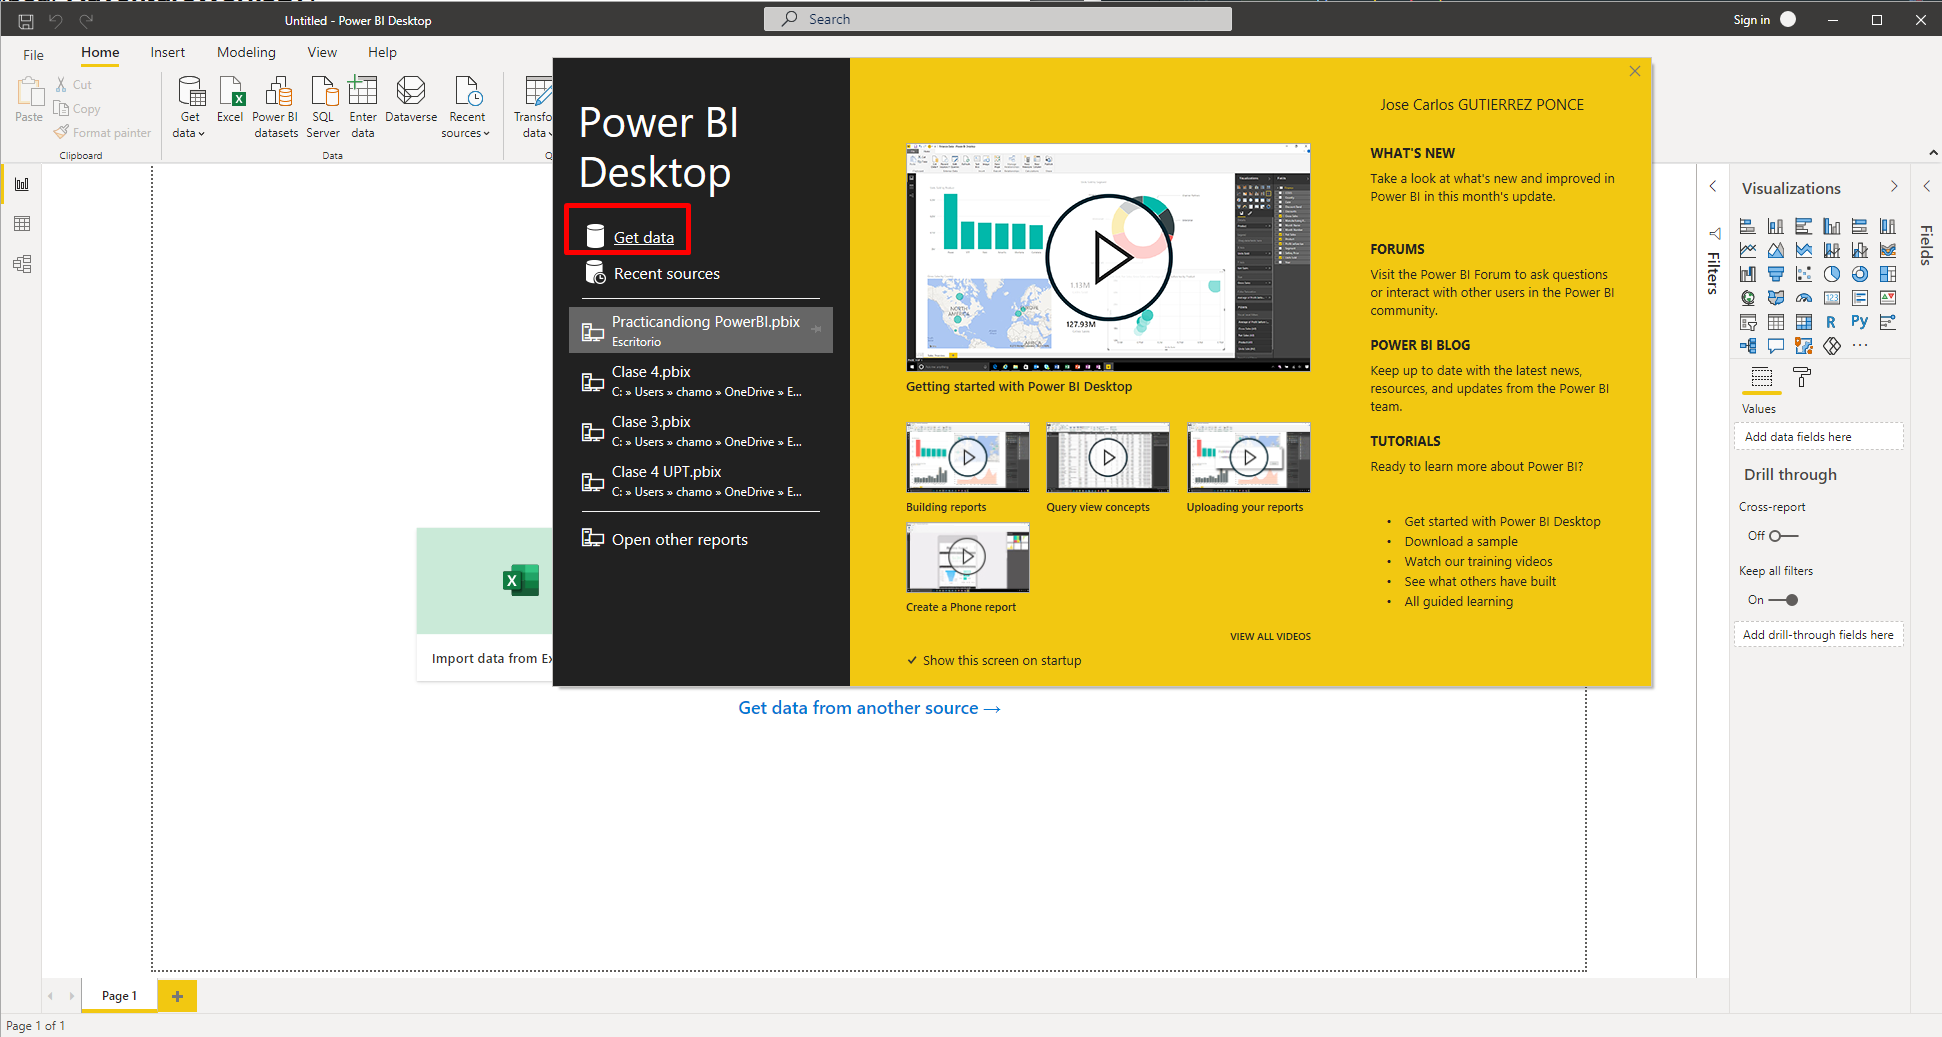
\includegraphics[width=14cm]{./images/5} 
	\end{center}

\textbf{1.6.En el cuadro Obtener Datos, click base de datos \textbf{Microsoft SQL}, y entonces click en Conectar.}

    \begin{center}
		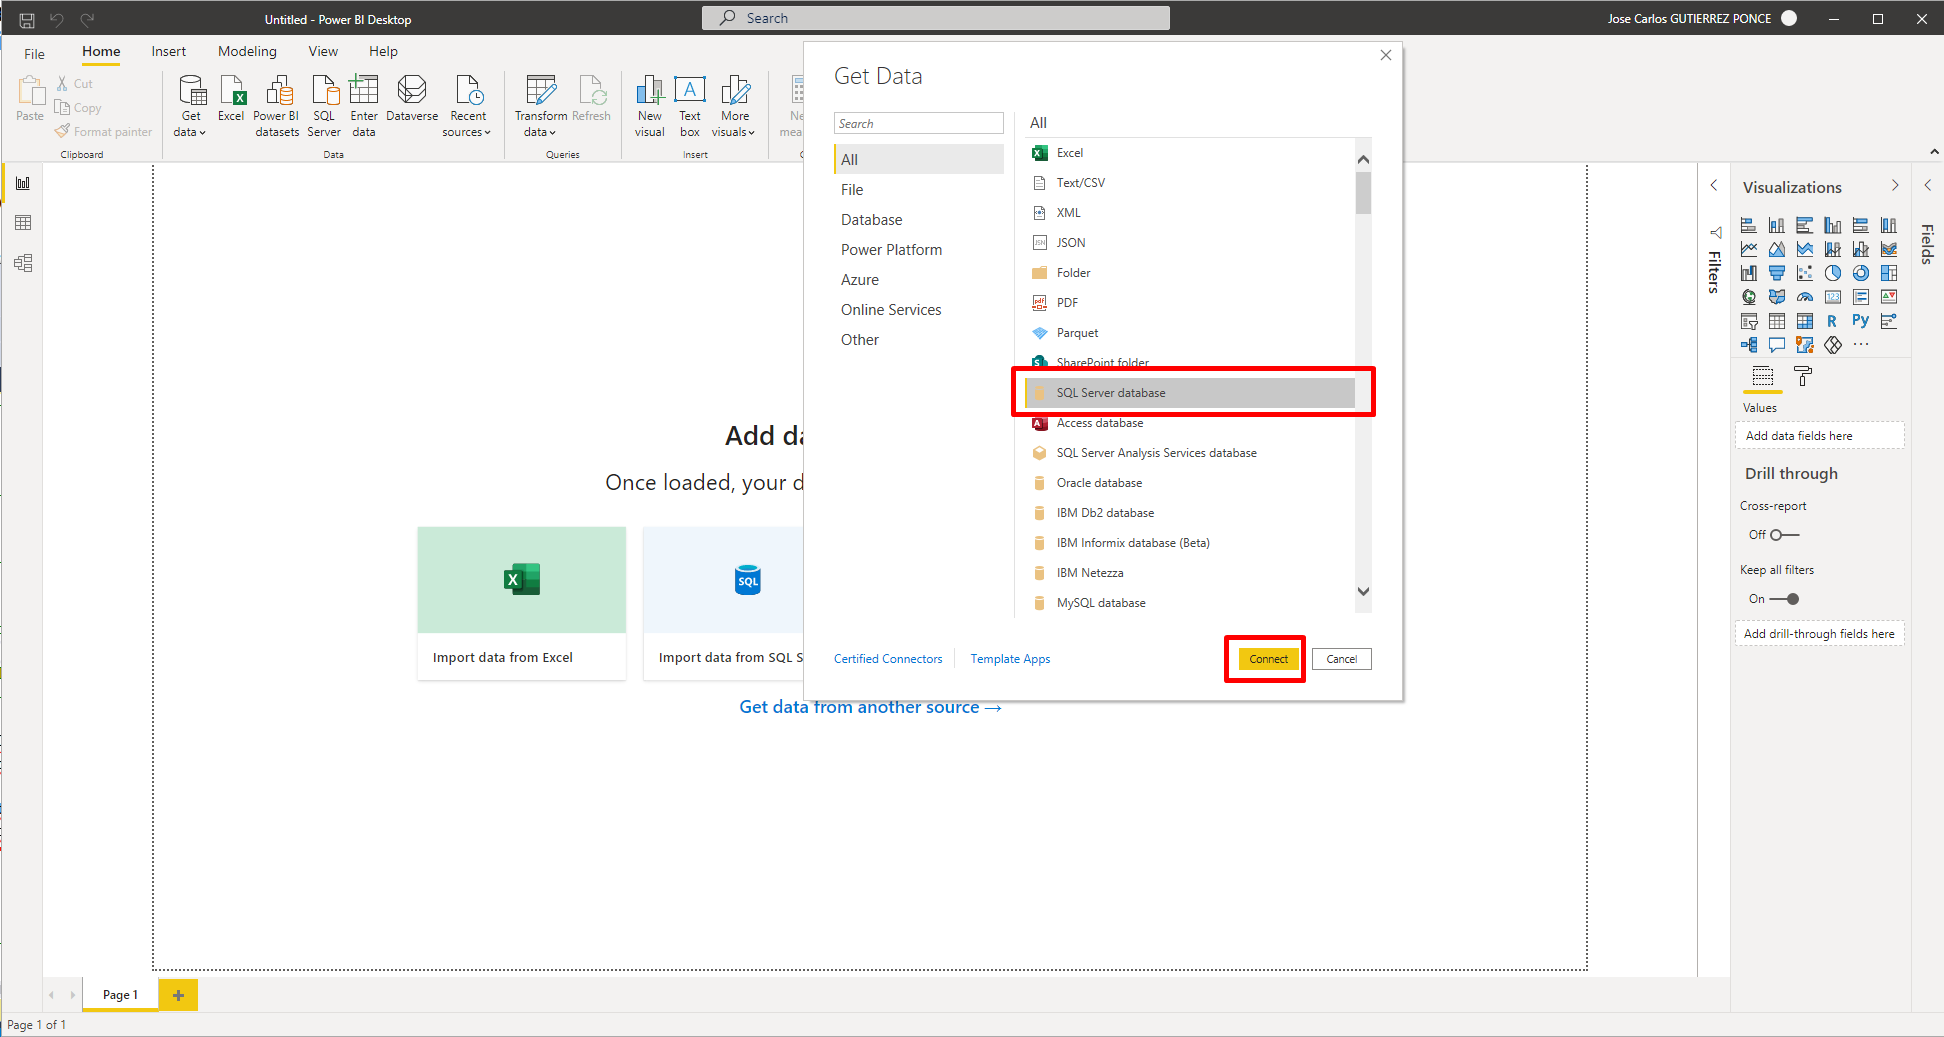
\includegraphics[width=14cm]{./images/6} 
	\end{center}
\newpage
\textbf{1.7. En la ventana base de datos Server database, En \textbf{Servidor}, escribir \textbf{(localhost)}.}

    \begin{center}
		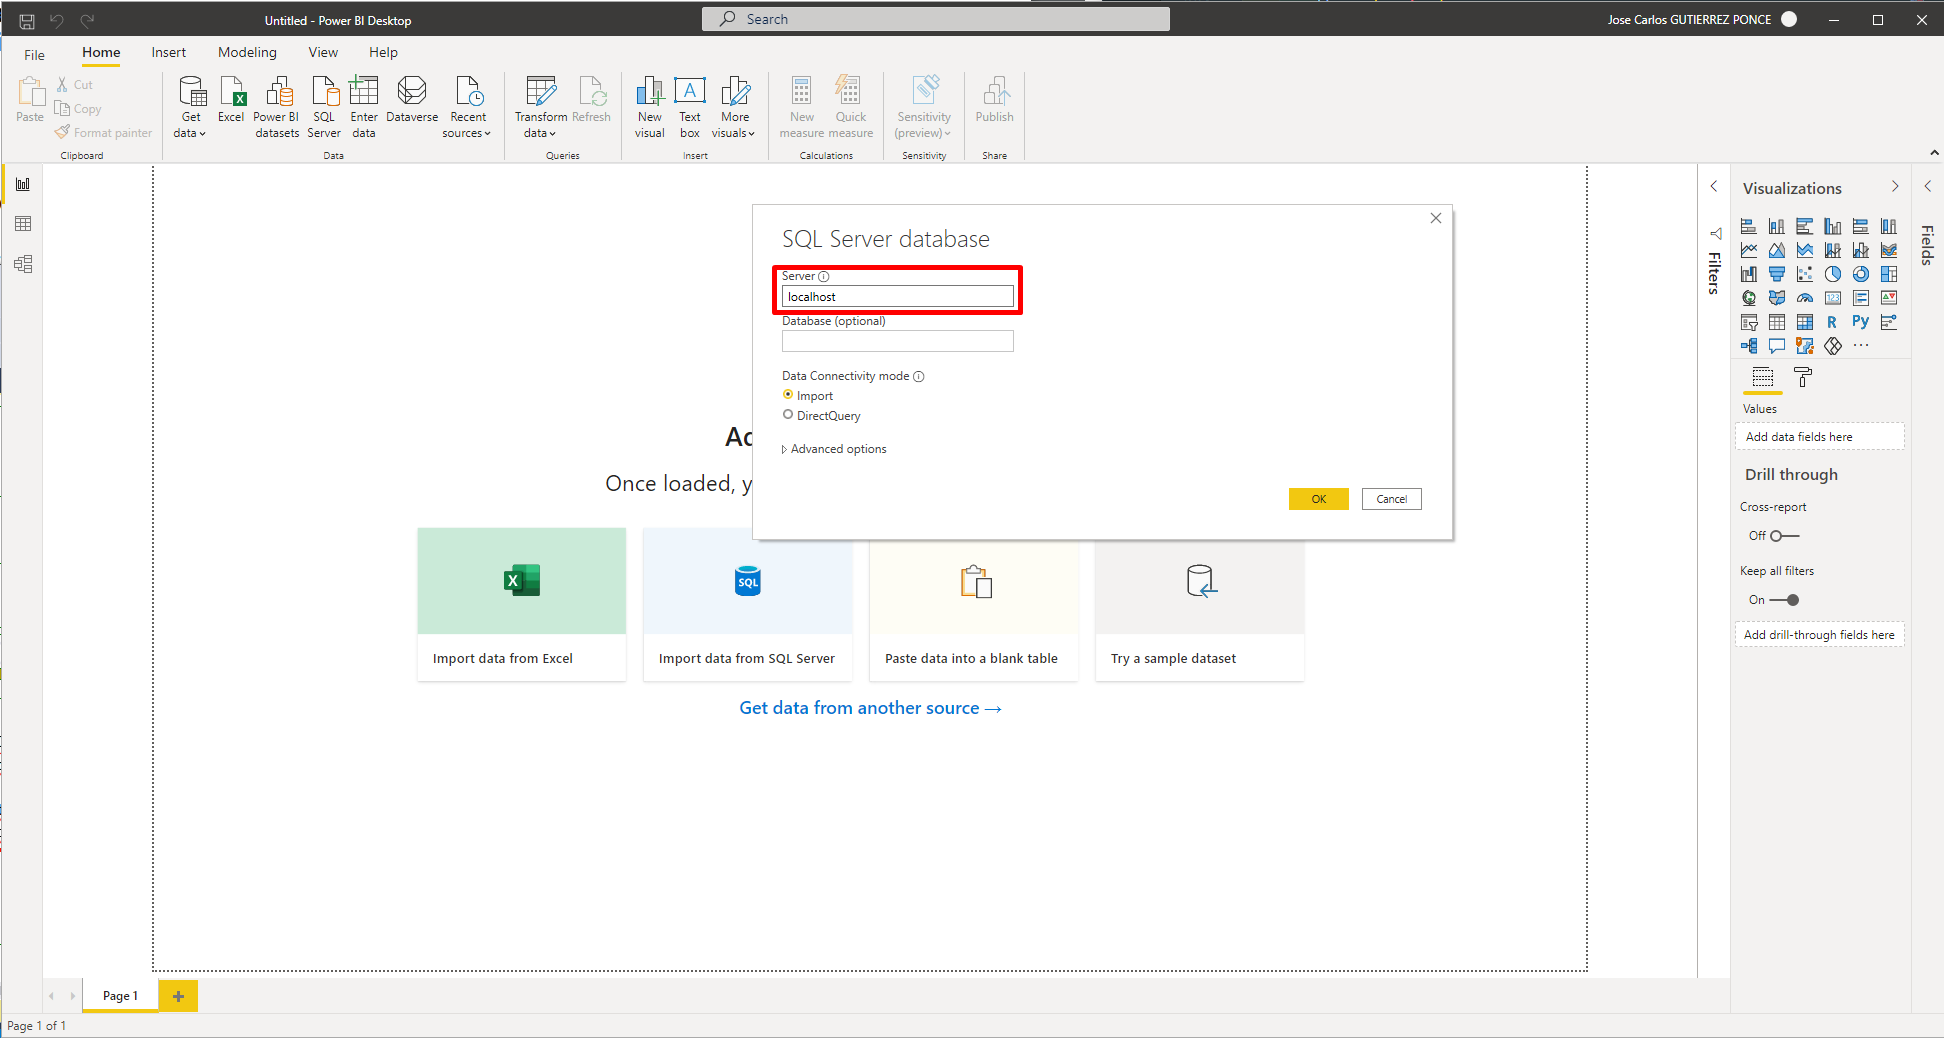
\includegraphics[width=14cm]{./images/7} 
	\end{center}

\textbf{1.8. En \textbf{Base de Datos (opcional)}, tipear \textbf{AdventureWorksLT2016}.}

    \begin{center}
		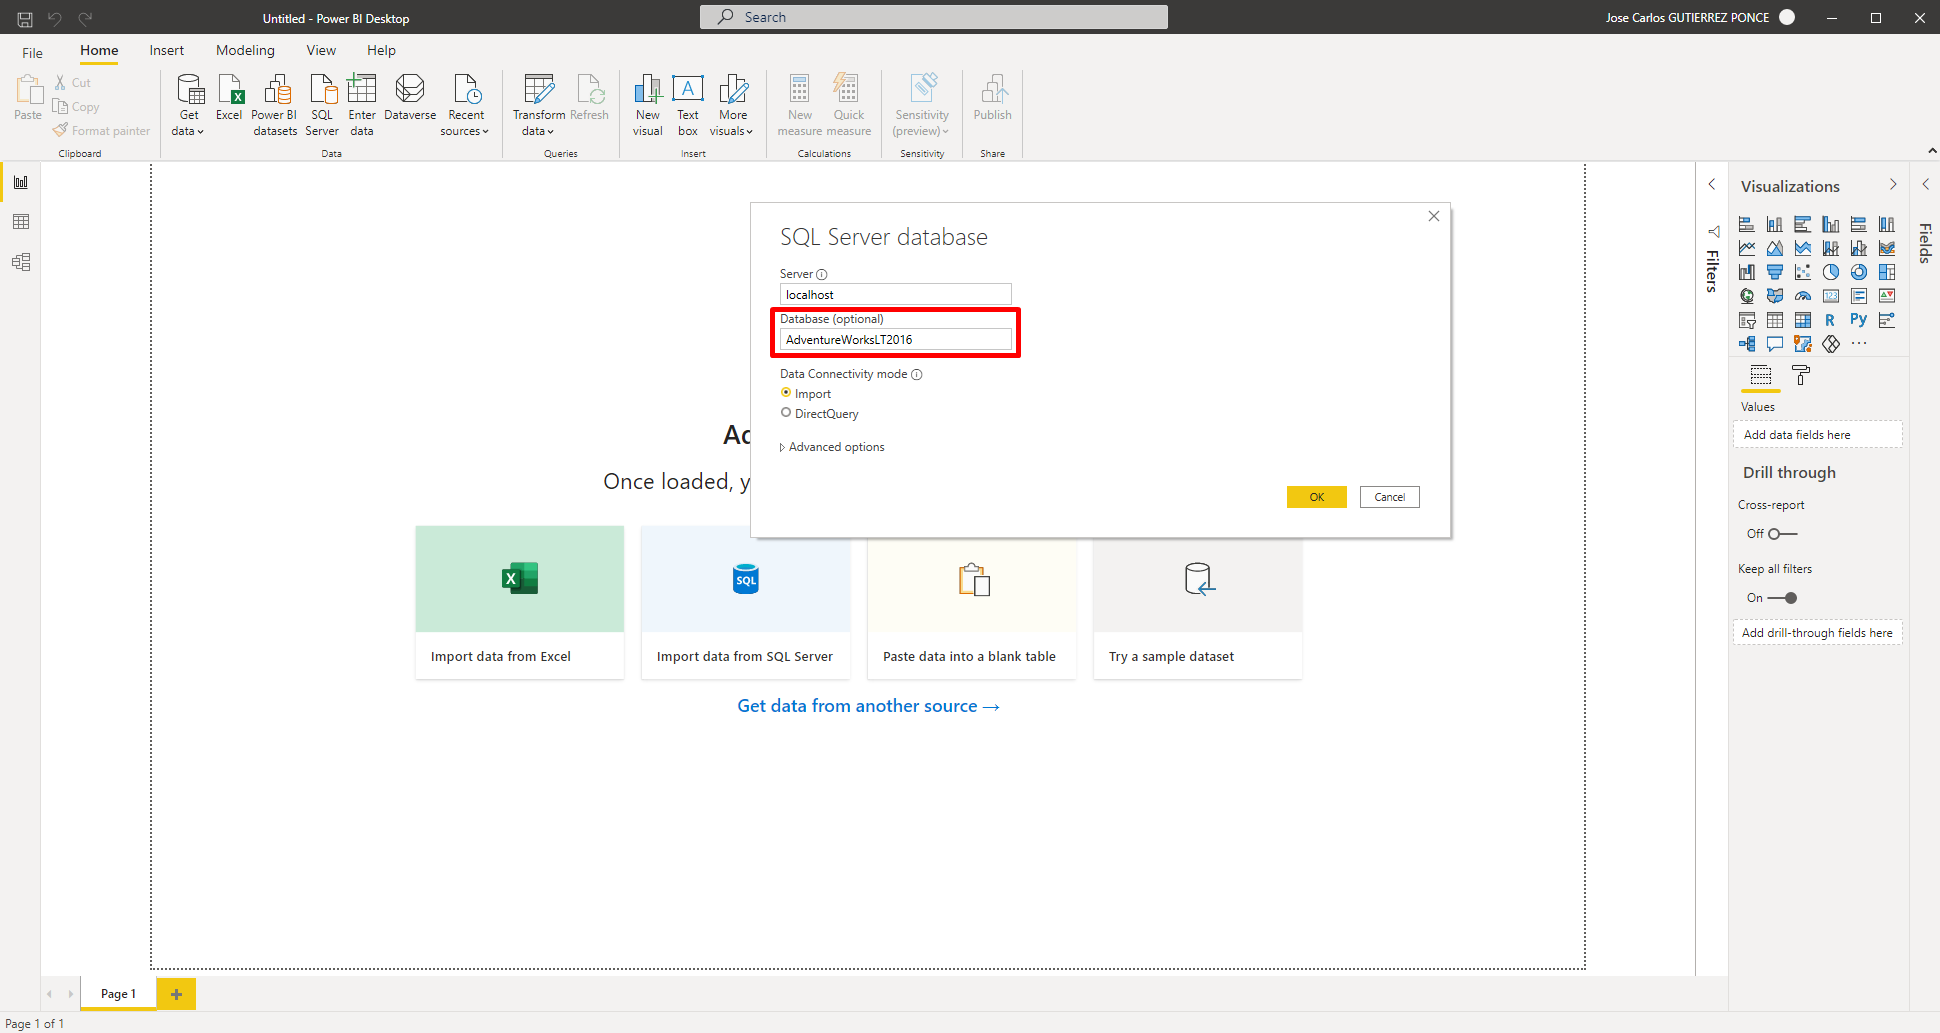
\includegraphics[width=14cm]{./images/8} 
	\end{center}
\newpage
\textbf{1.9. Expandir el cuadro \textbf{Opciones Avanzadas}. Copiar el script \textbf{Task 1} del archivo \textbf{Lab Exercise 1.sql}. y pegar 
la consulta en Power BI, en el cuadro sentencia SQL. Luego presionar OK.}

    \begin{center}
		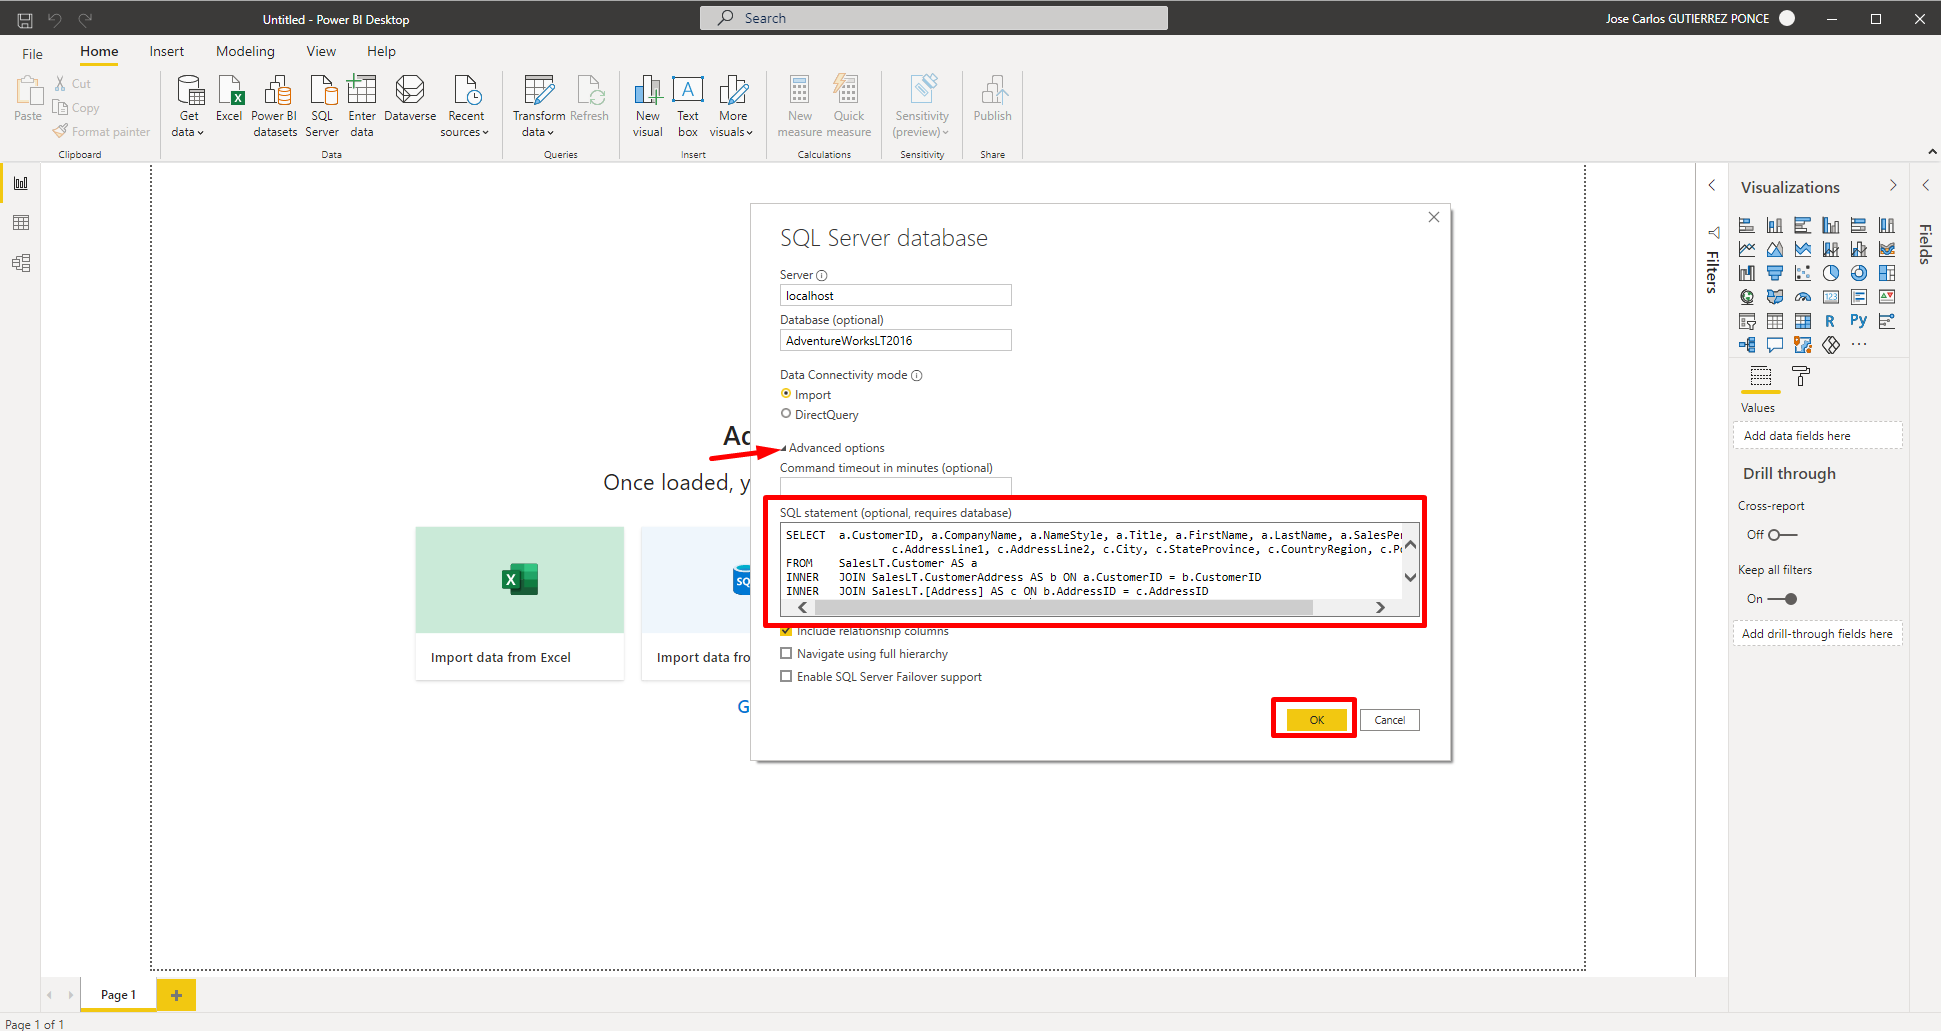
\includegraphics[width=14cm]{./images/9} 
	\end{center}

\textbf{1.10. En la ventana de vista prDelete click en \textbf{Load}.}

    \begin{center}
		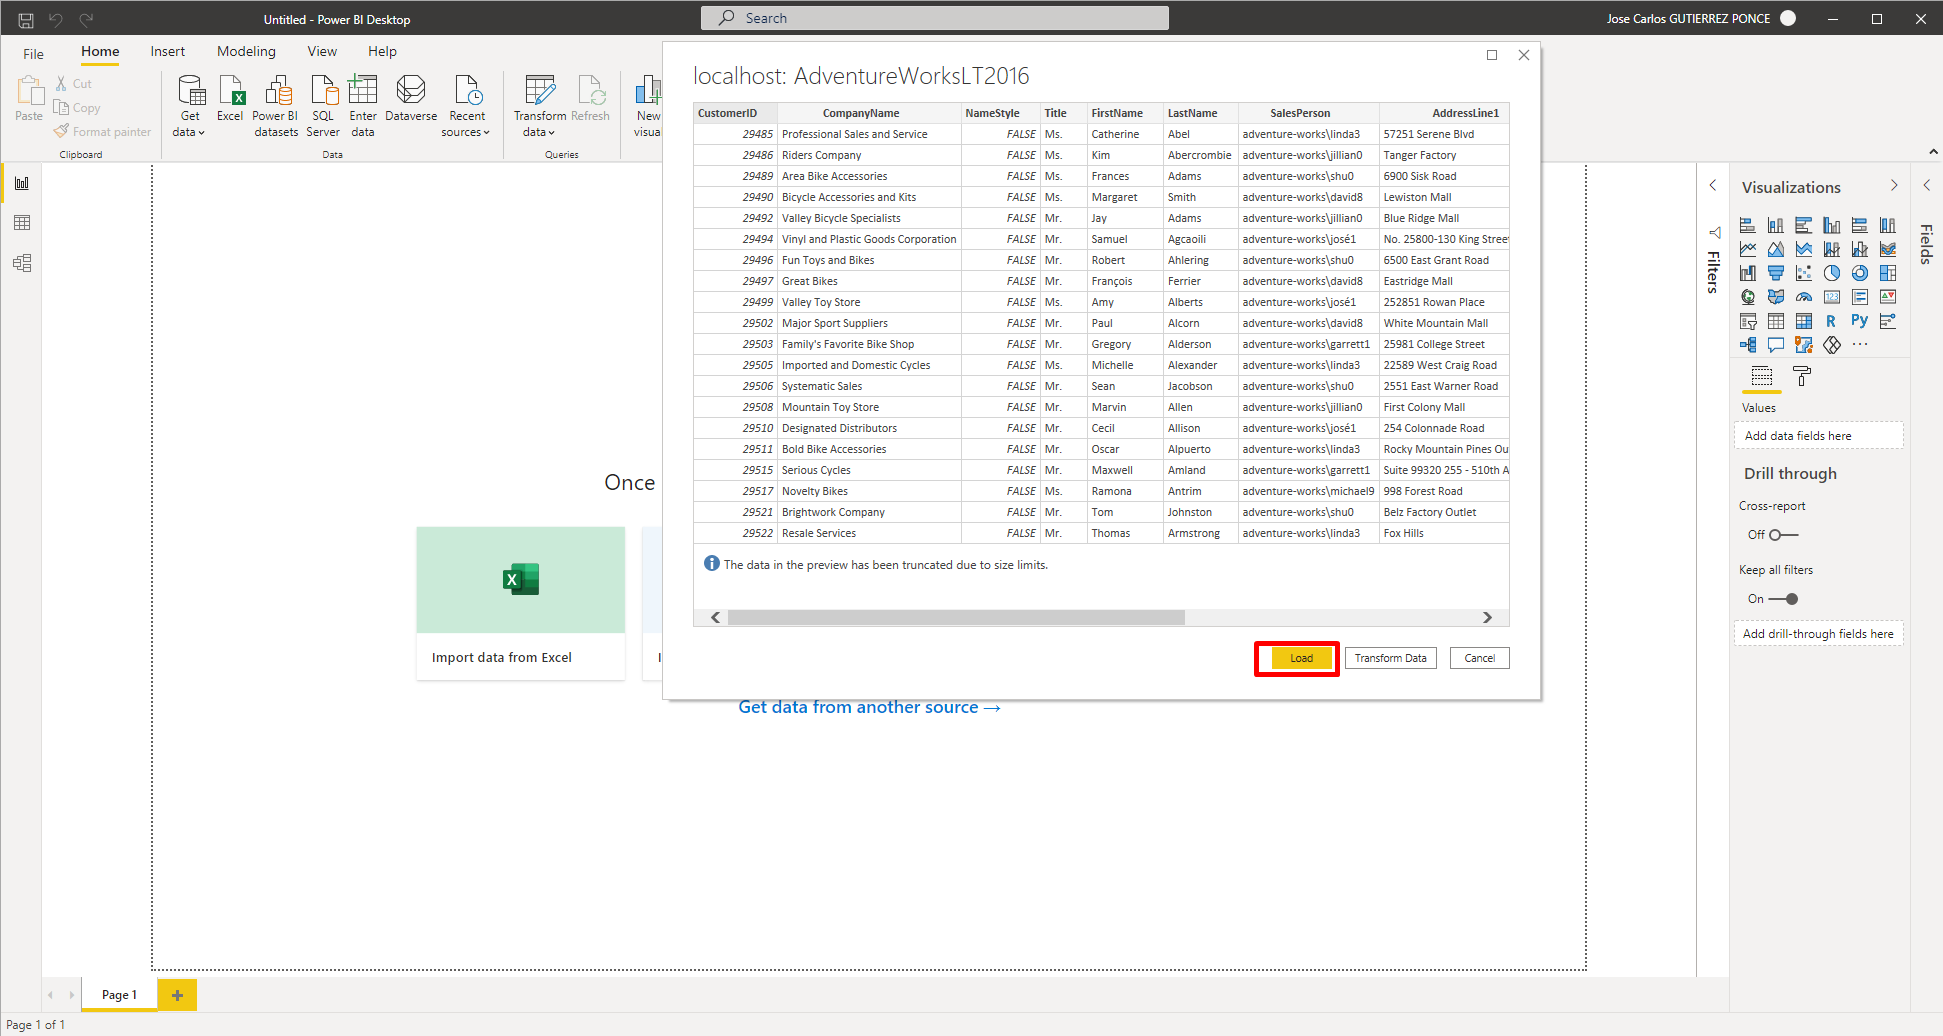
\includegraphics[width=14cm]{./images/10} 
	\end{center}
\newpage
\textbf{1.11. En Power BI Desktop, click \textbf{Obtener Datos} y luego click en Mas.}

    \begin{center}
		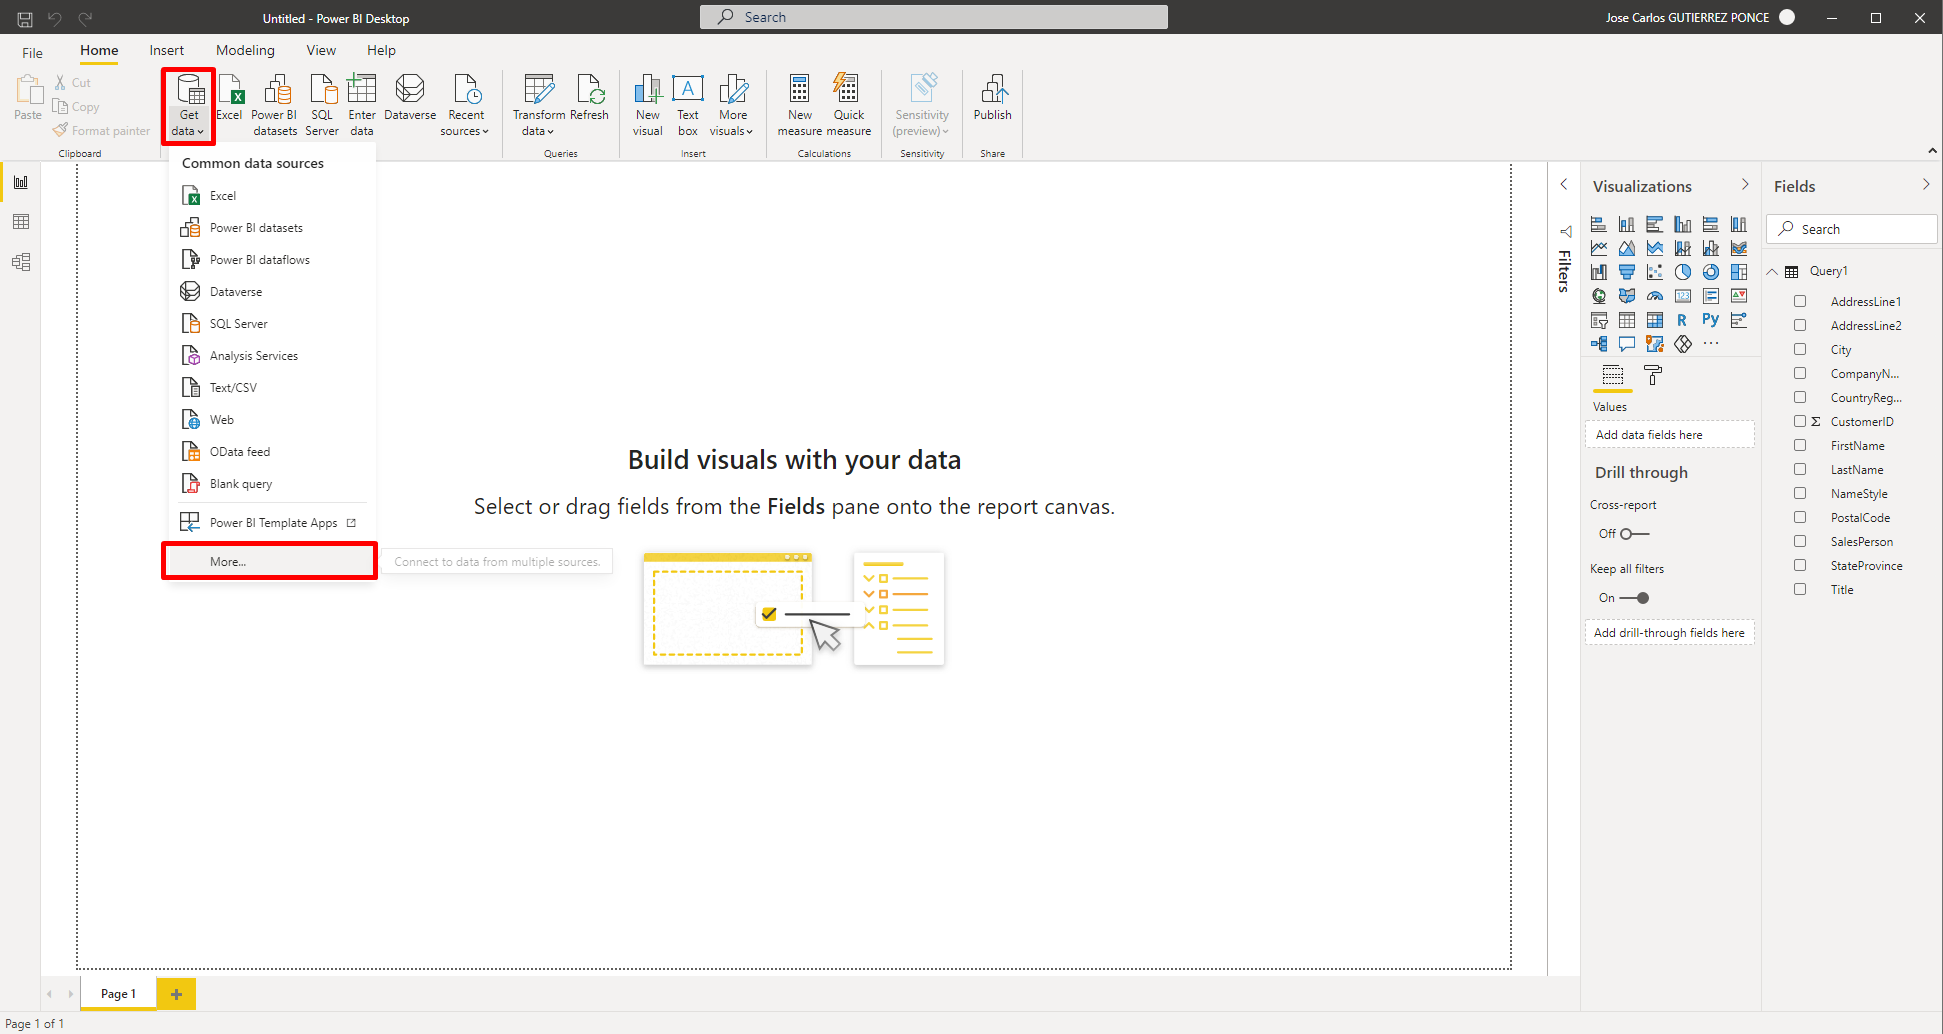
\includegraphics[width=14cm]{./images/11} 
	\end{center}

\textbf{1.12. Repetir los pasos del 6 al 10, utilizando el script \textbf{Task 2}.}

    \begin{center}
		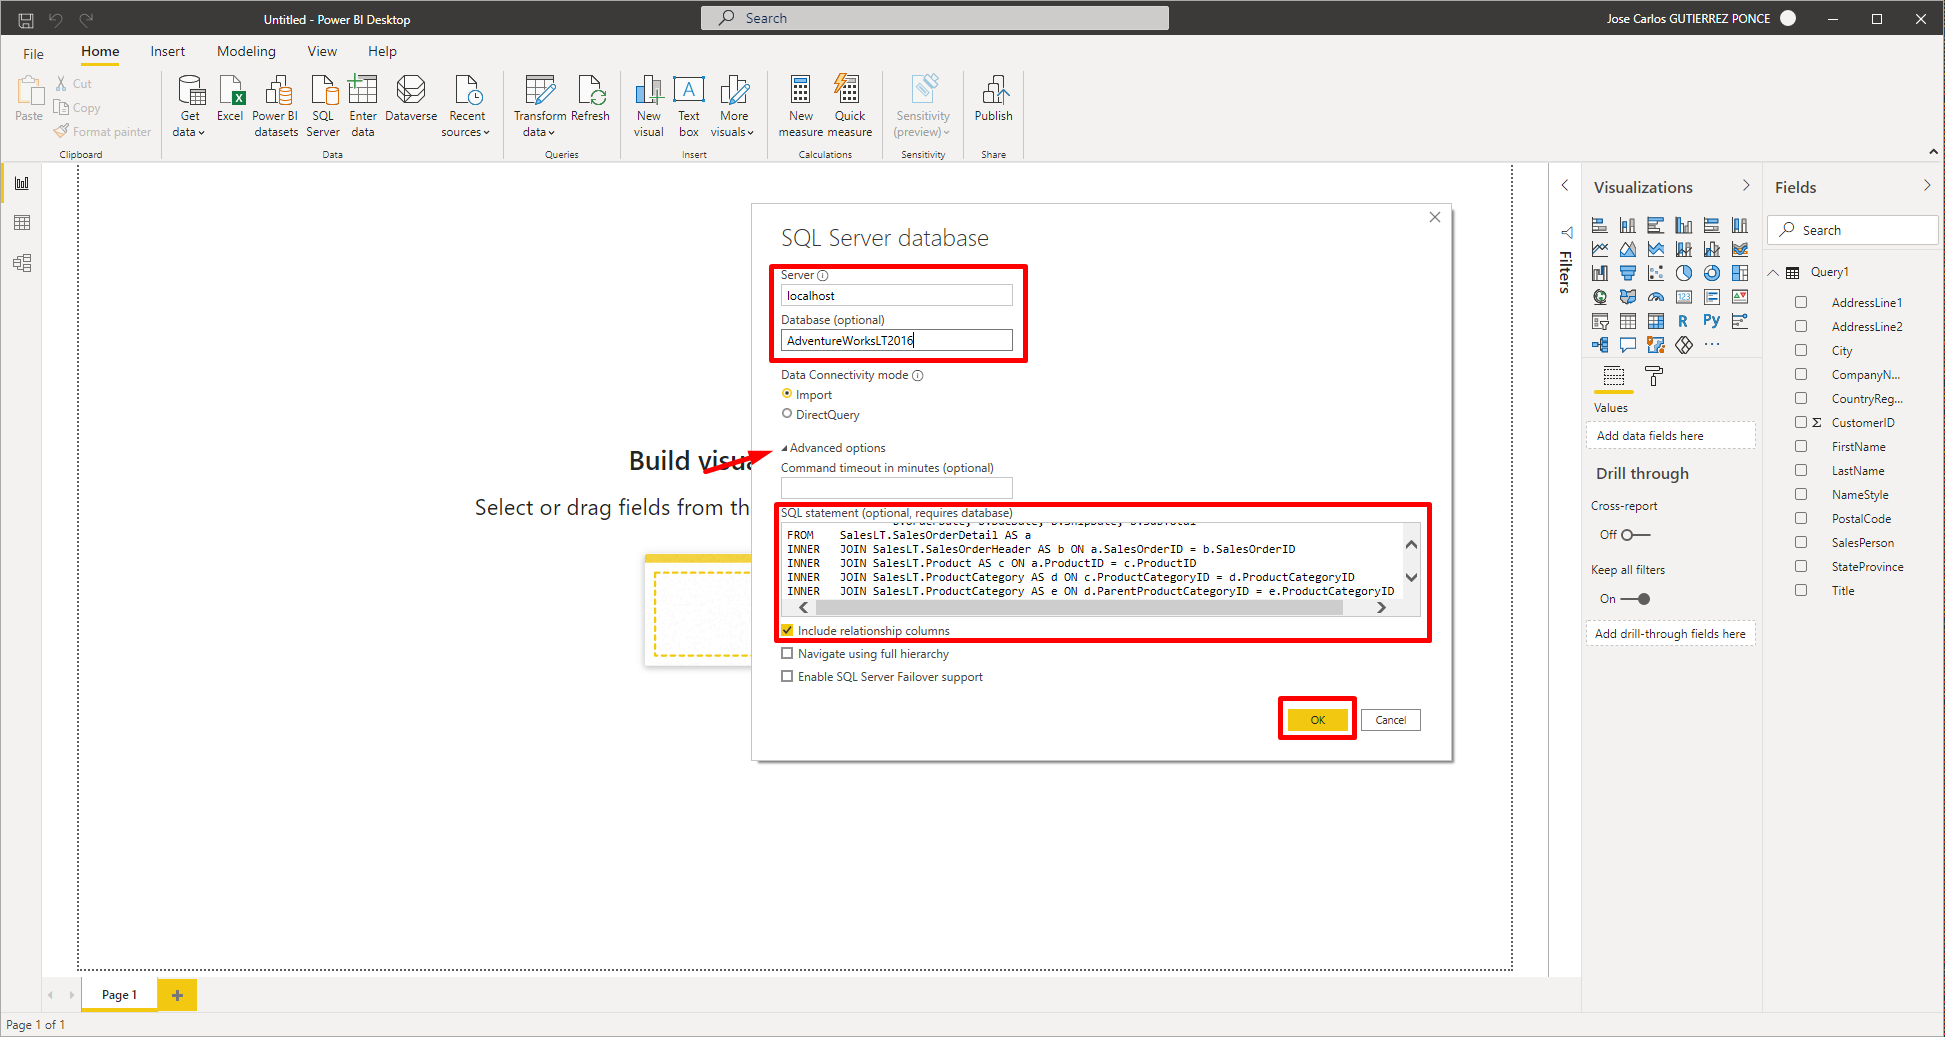
\includegraphics[width=14cm]{./images/12} 
	\end{center}
\newpage
\textbf{1.13. De regreso en el reporte. Guardar el archivo como \textbf{AdventureWorksLT Sales.pbix}.}

    \begin{center}
		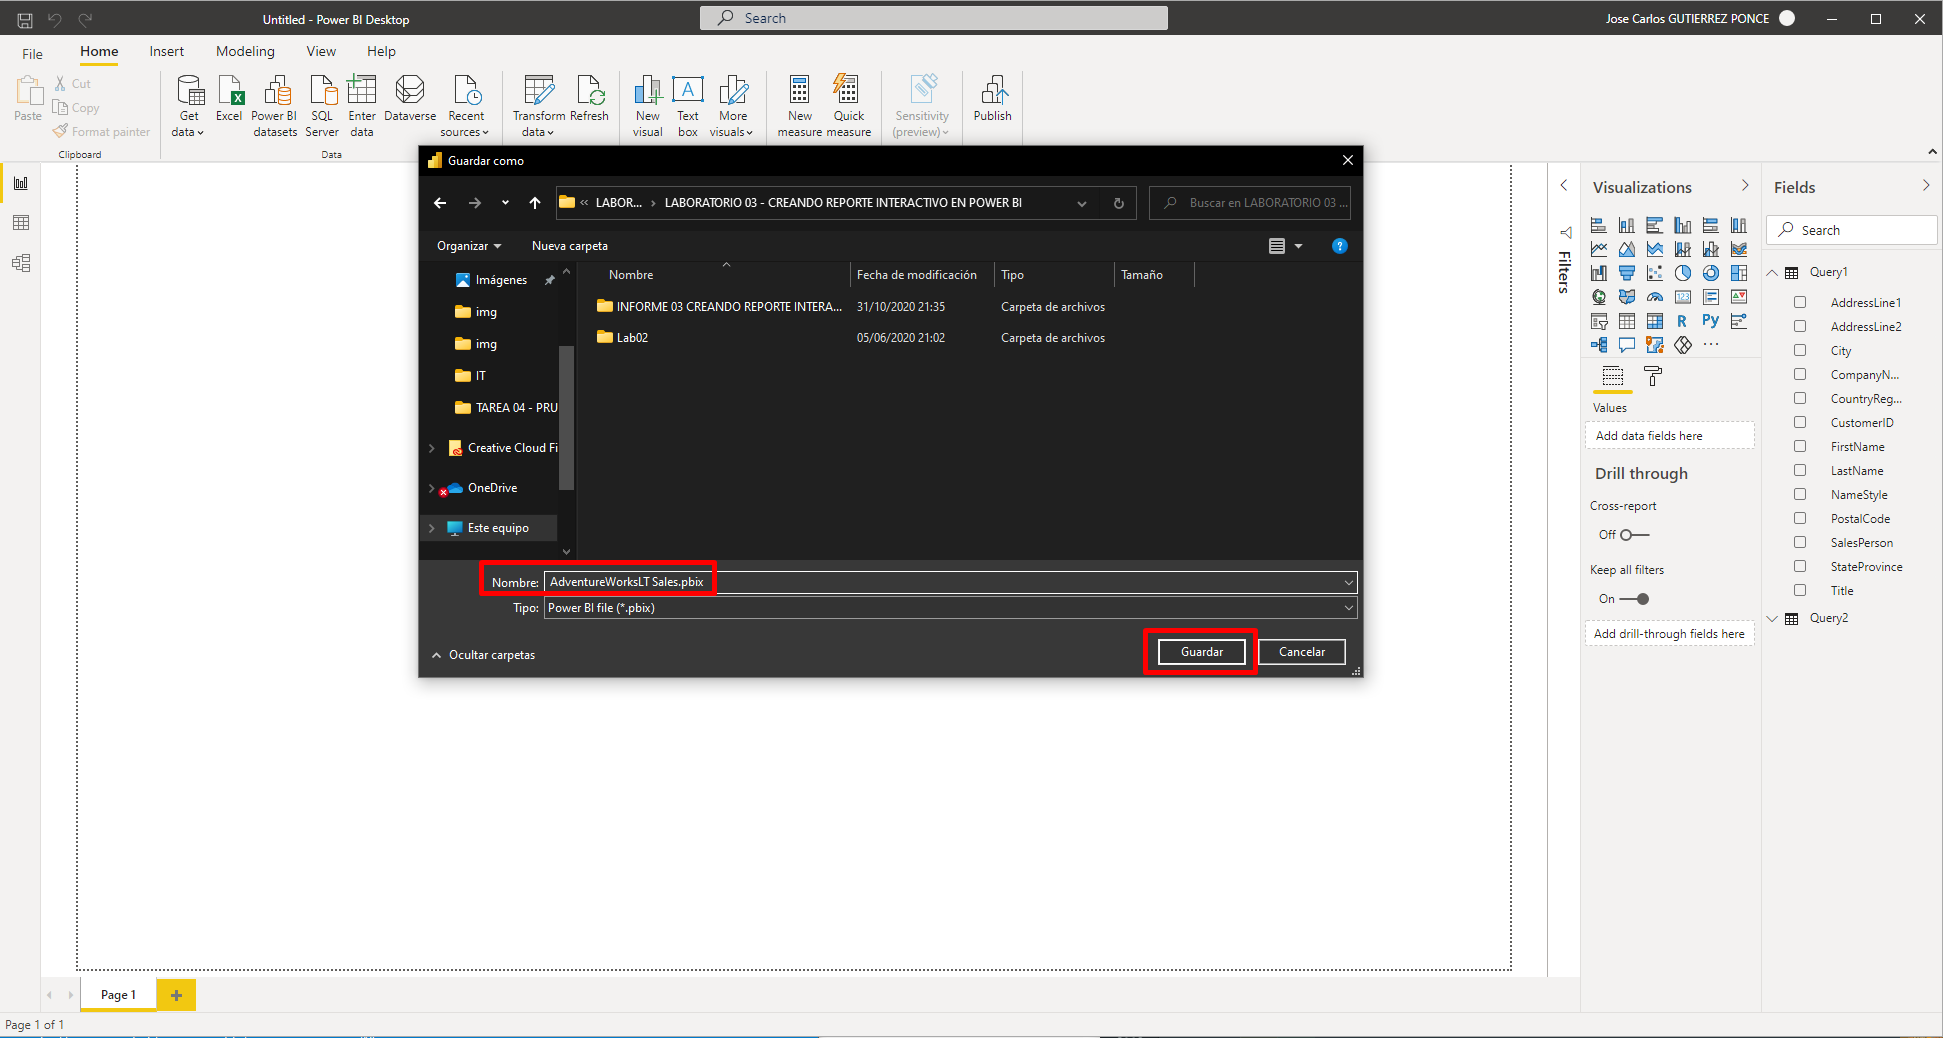
\includegraphics[width=14cm]{./images/13} 
	\end{center}



\newpage

\section{Graficar Datos}

\textbf{2.1. En el panel \textbf{Fields} \textbf{(Fields)}, click derecho sobre \textbf{Query1}, clic en \textbf{Rename}, tipear \textbf{Customers} y presionar Enter.}

    \begin{center}
		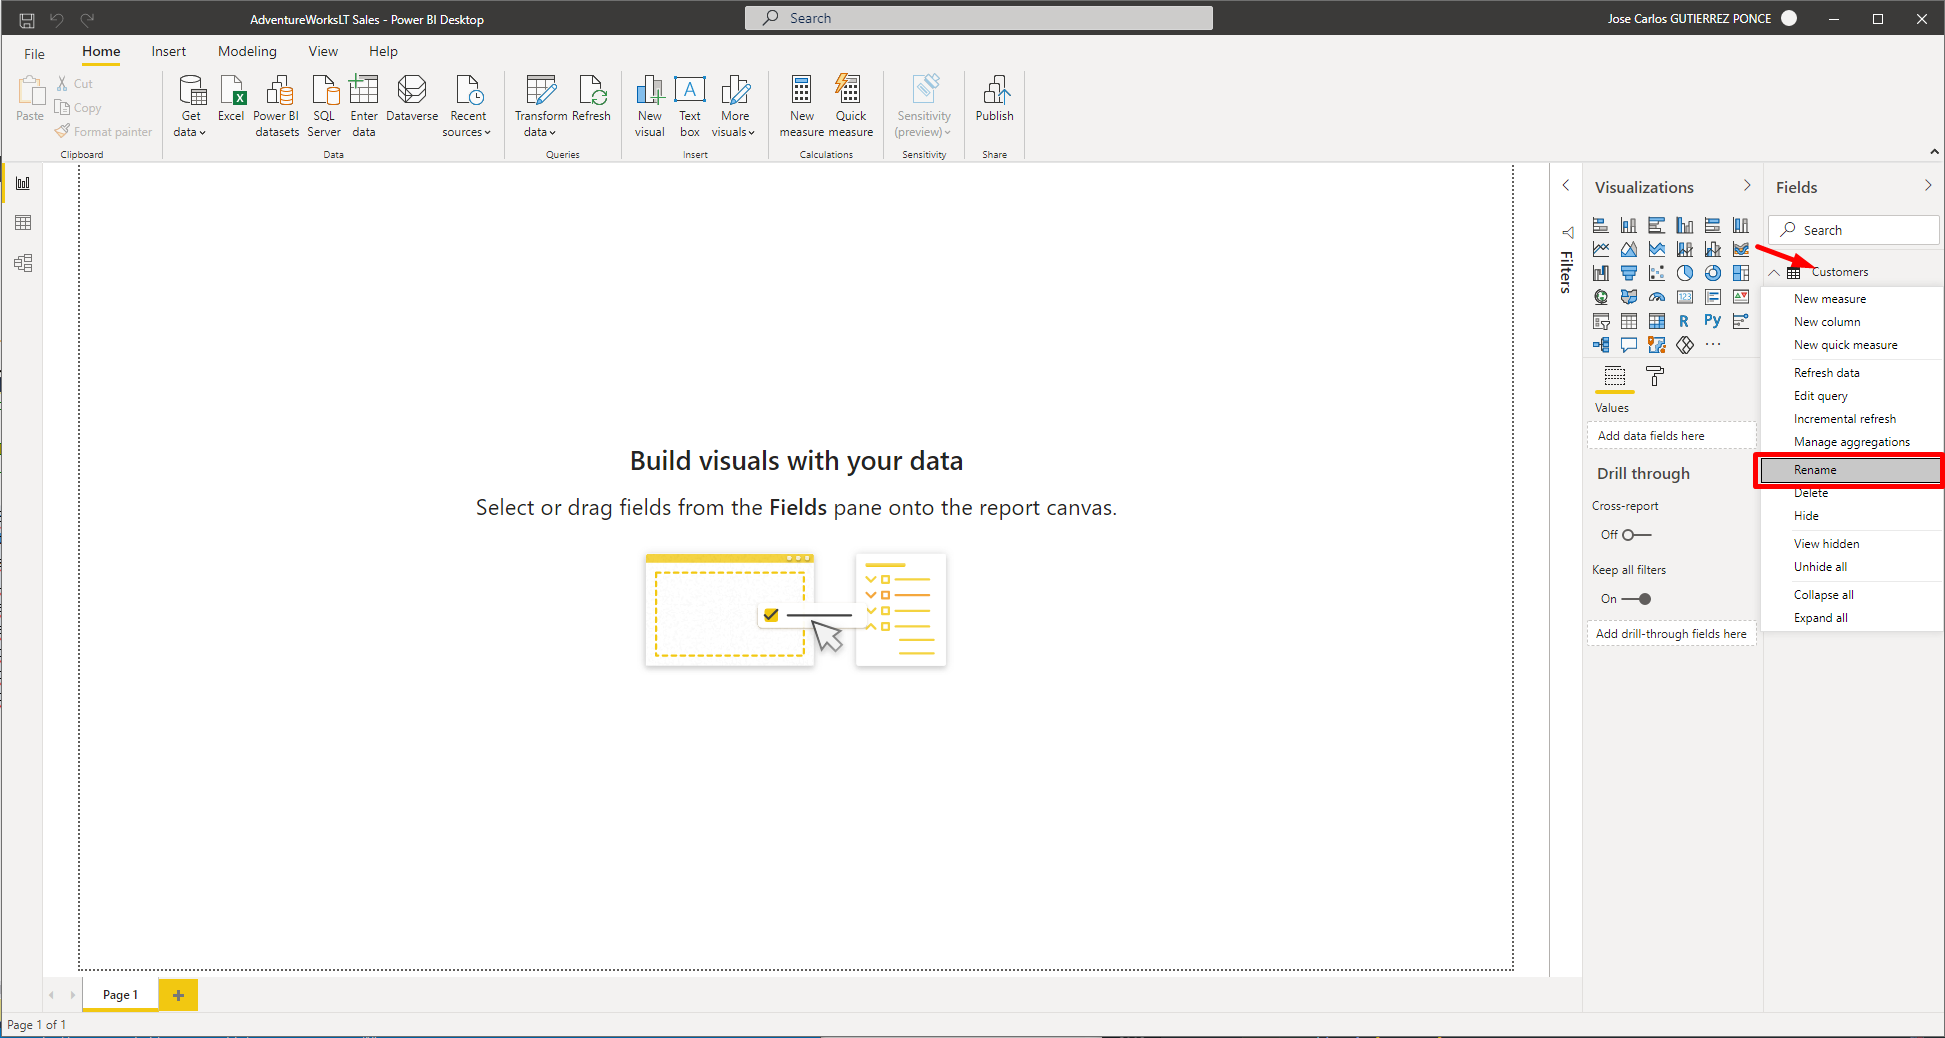
\includegraphics[width=14cm]{./images/14} 
	\end{center}
	
\textbf{2.2. Haga clic con el botón derecho en \textbf{Query2}, haga clic en \textbf{Rename}, escriba \textbf{Sales} y, a continuación, presione Enter.}

    \begin{center}
		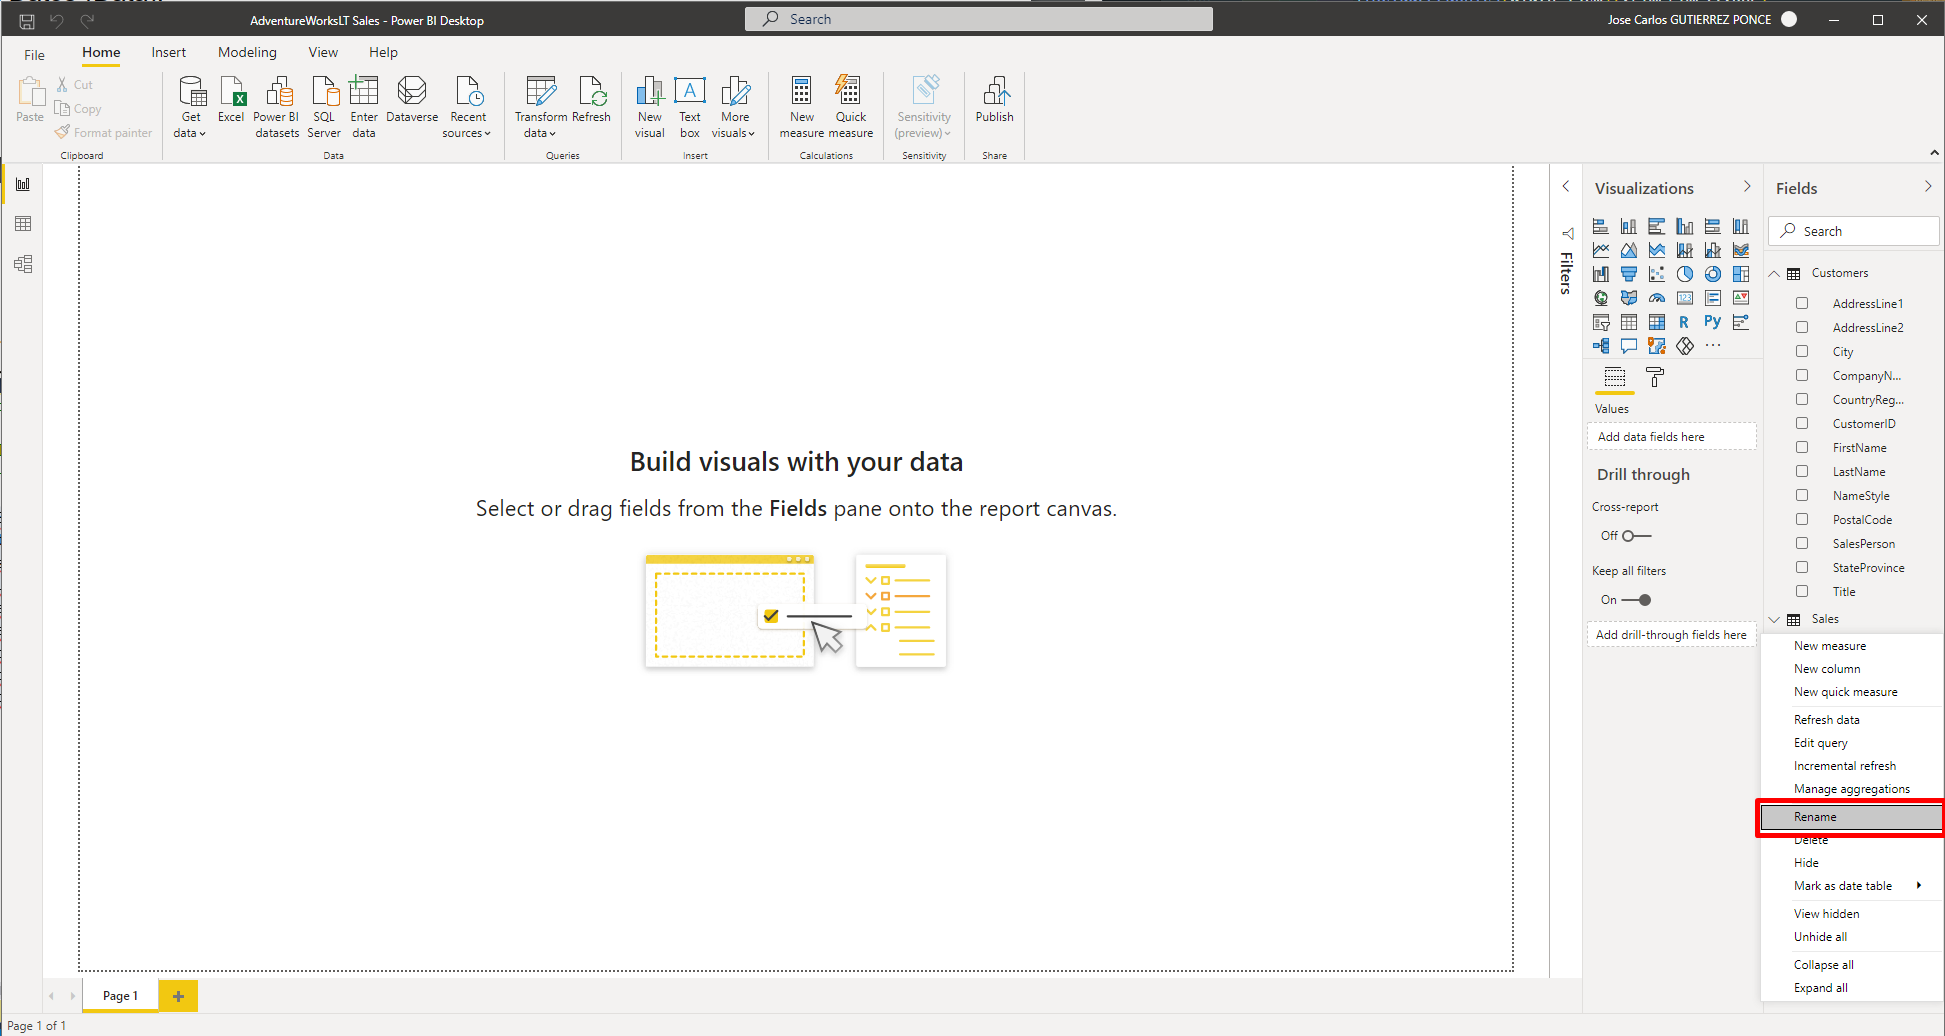
\includegraphics[width=14cm]{./images/15} 
	\end{center}
	
\textbf{2.3.Expanda las dos tablas para mostrar todos los \textbf{Fields}.}

    \begin{center}
		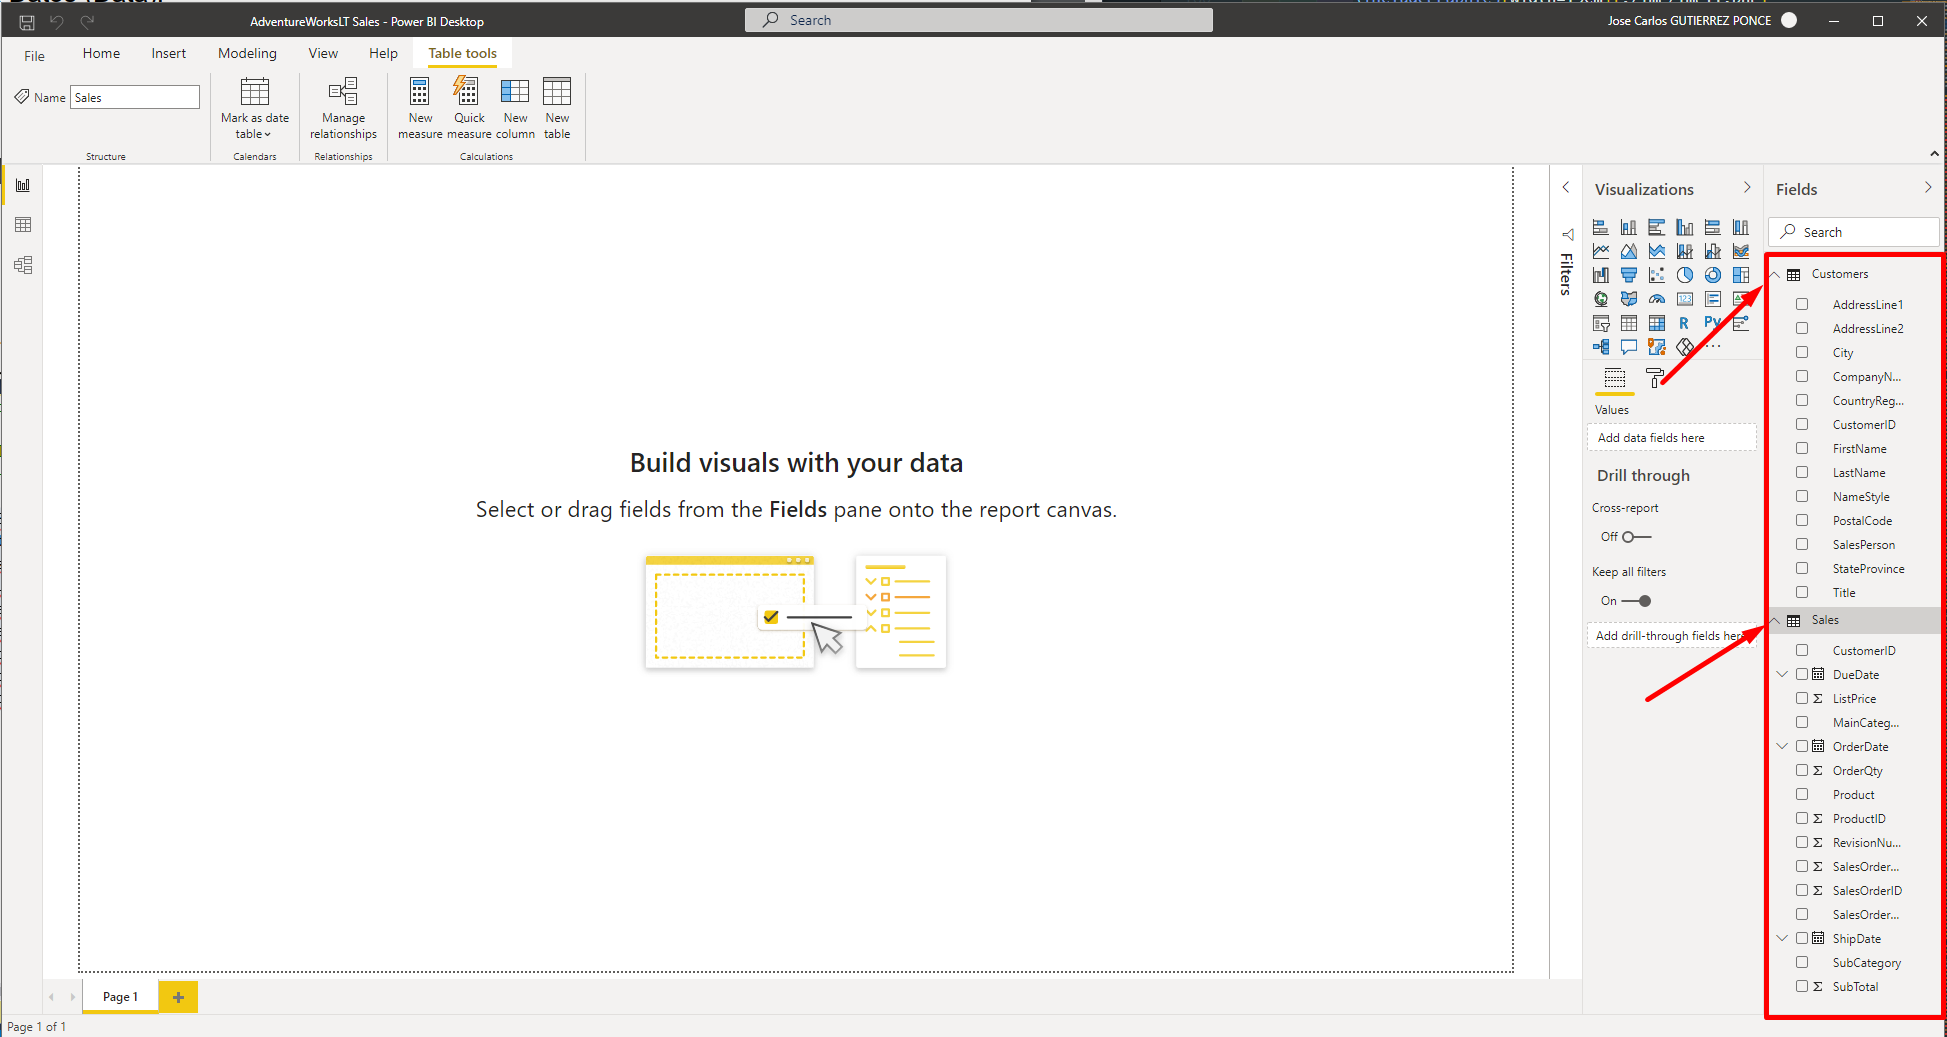
\includegraphics[width=14cm]{./images/16} 
	\end{center}
	
\textbf{2.4. En la barra de navegación izquierda, haga clic en \textbf{Data}.}

    \begin{center}
		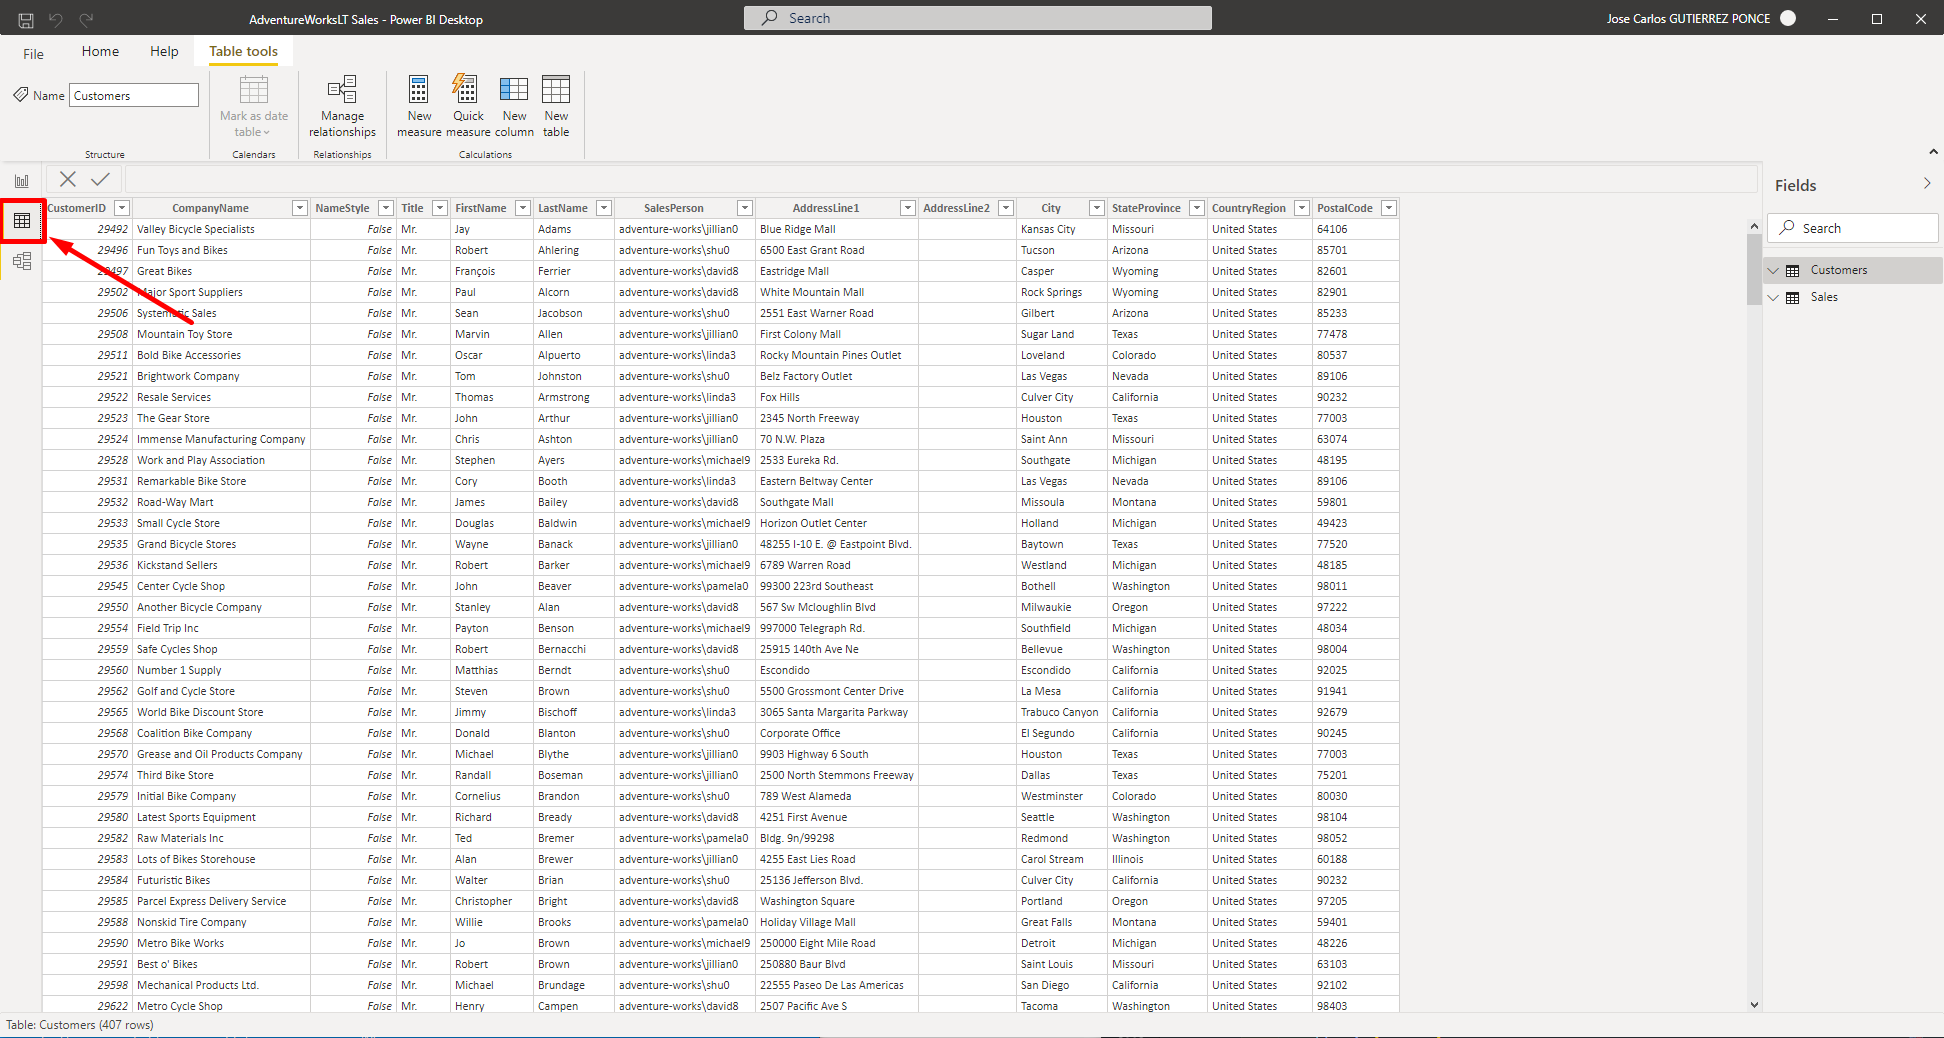
\includegraphics[width=14cm]{./images/17} 
	\end{center}
 \newpage
\textbf{2.5.En el panel \textbf{Fields} \textbf{(Fields)}, haga clic en la tabla Customers, si aún no está seleccionada.}

    \begin{center}
		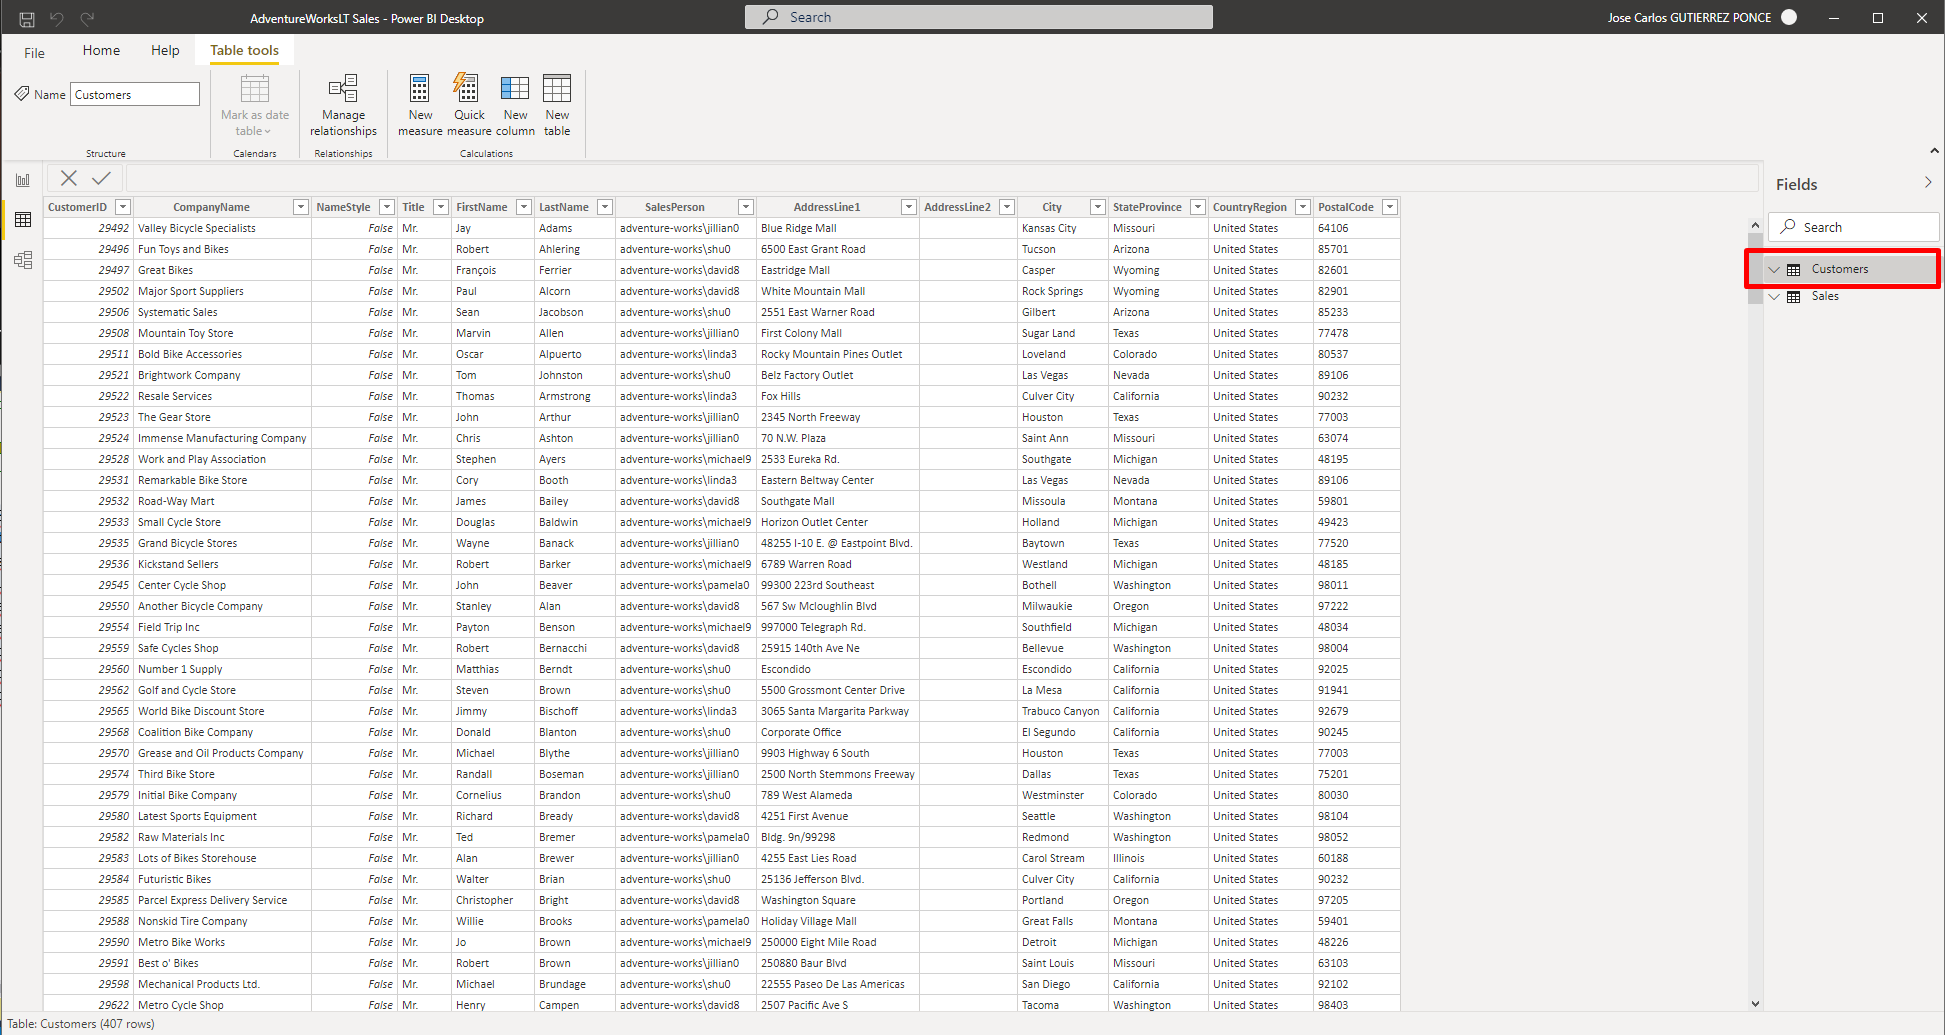
\includegraphics[width=14cm]{./images/18} 
	\end{center}
	
\textbf{2.6. Haga clic con el botón derecho en la columna \textbf{NameStyle} y haga clic en \textbf{Delete}.}

    \begin{center}
		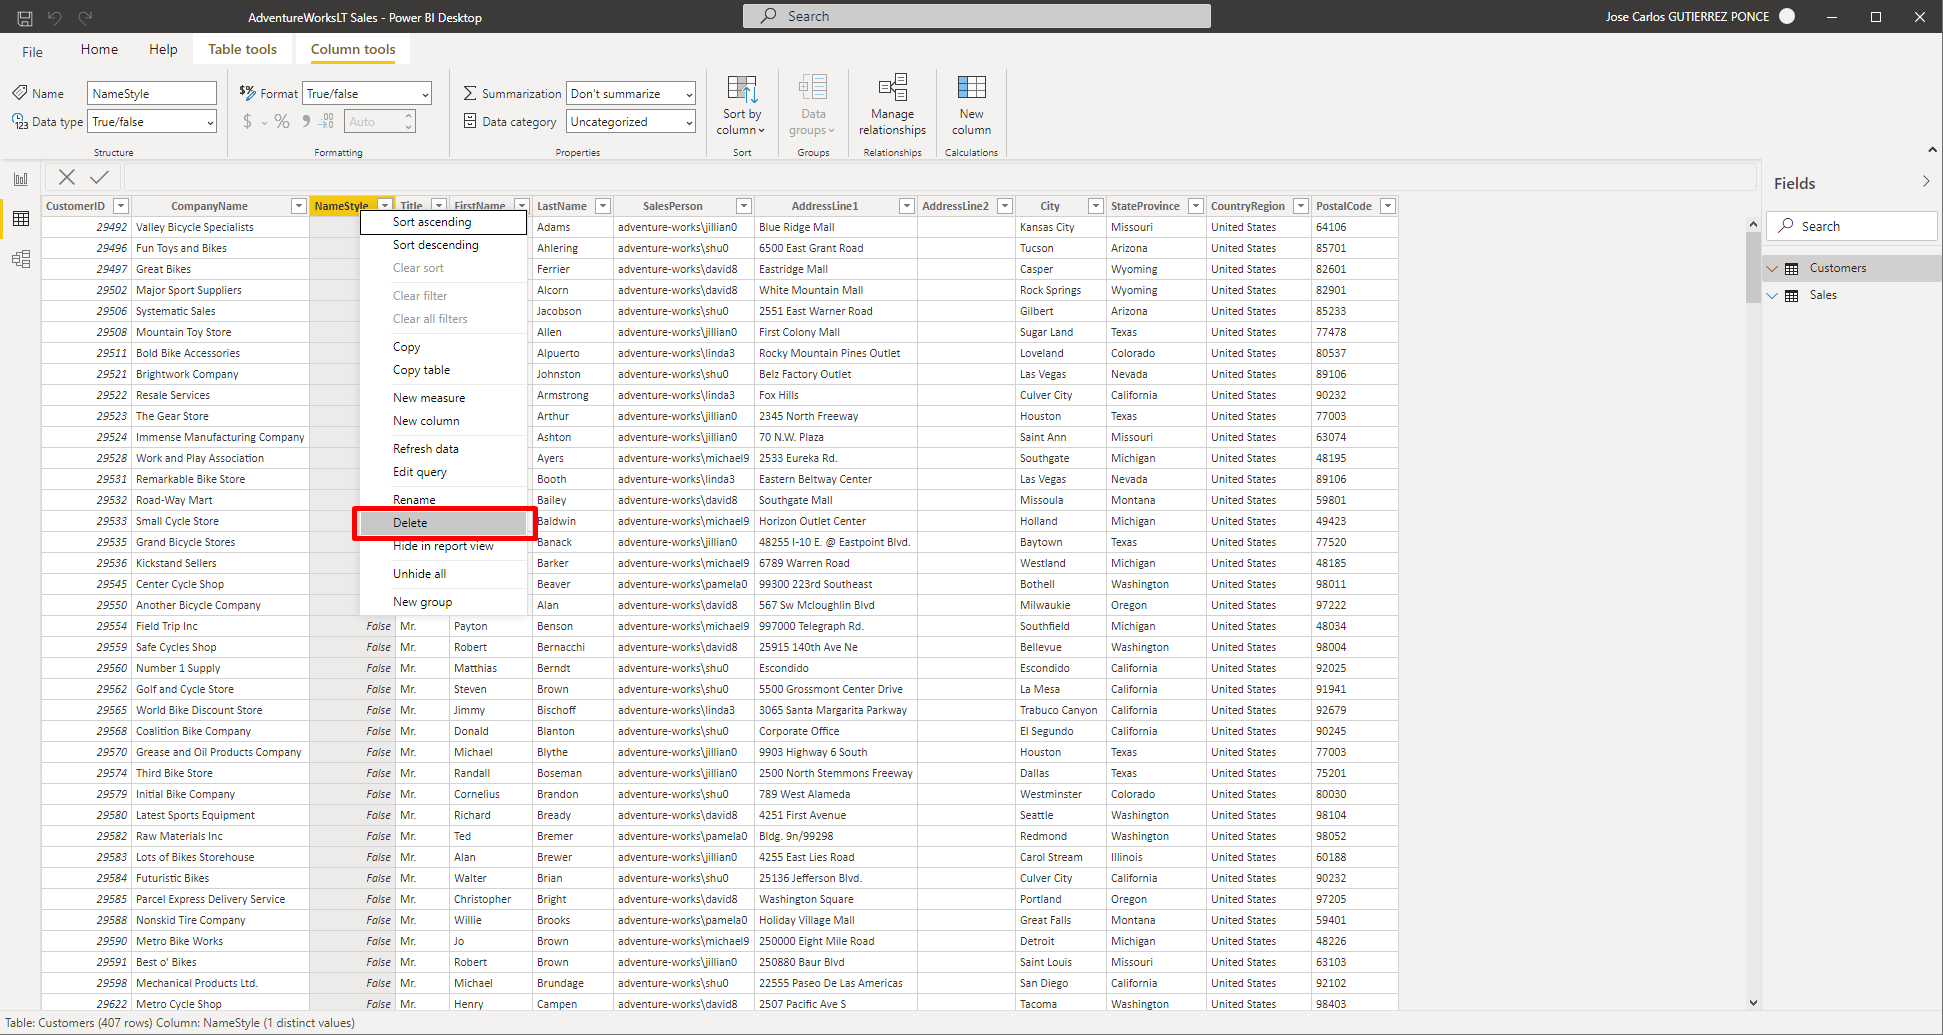
\includegraphics[width=14cm]{./images/19} 
	\end{center}
\newpage	
\textbf{2.7. En el cuadro de diálogo \textbf{Delete Column}, haga clic en \textbf{Delete}.}

    \begin{center}
		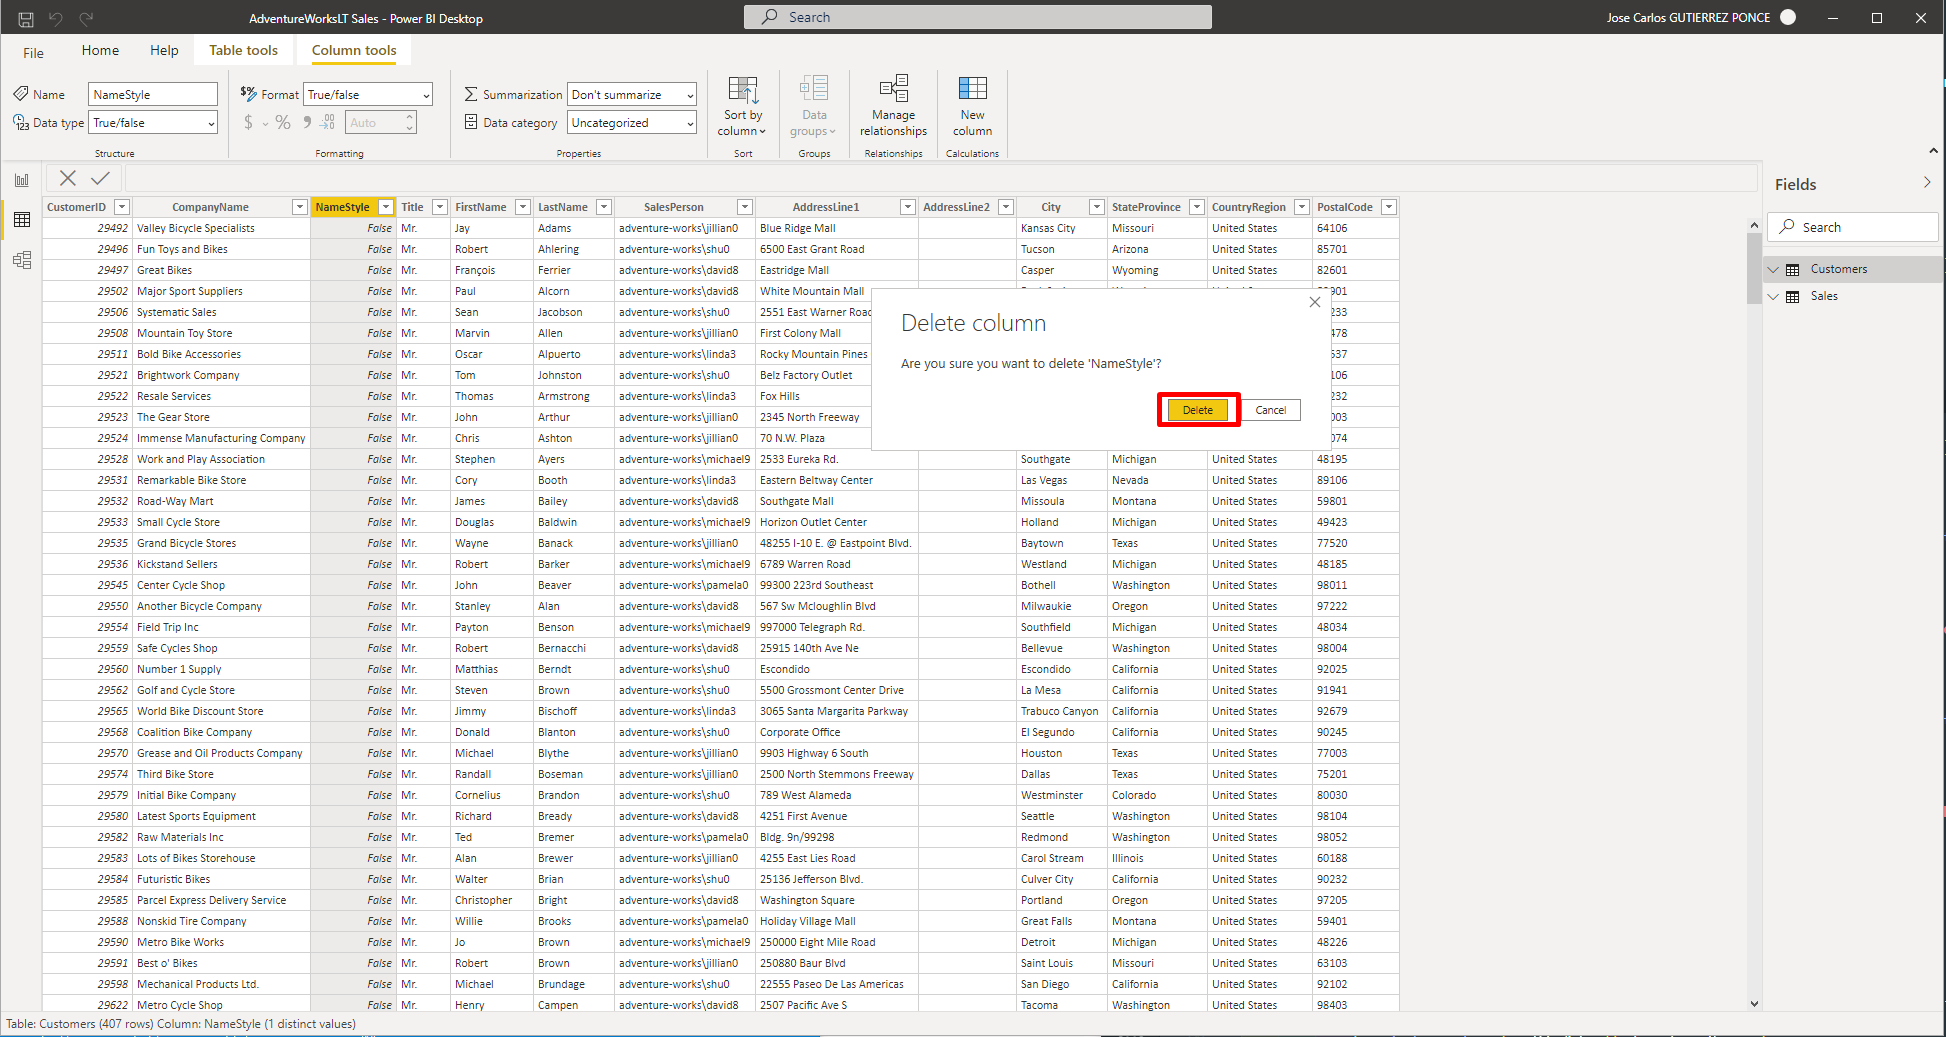
\includegraphics[width=14cm]{./images/20} 
	\end{center}
	
\textbf{2.8. Haga clic con el botón derecho en la columna \textbf{SalesPerson} y haga clic en \textbf{Delete}.}

    \begin{center}
		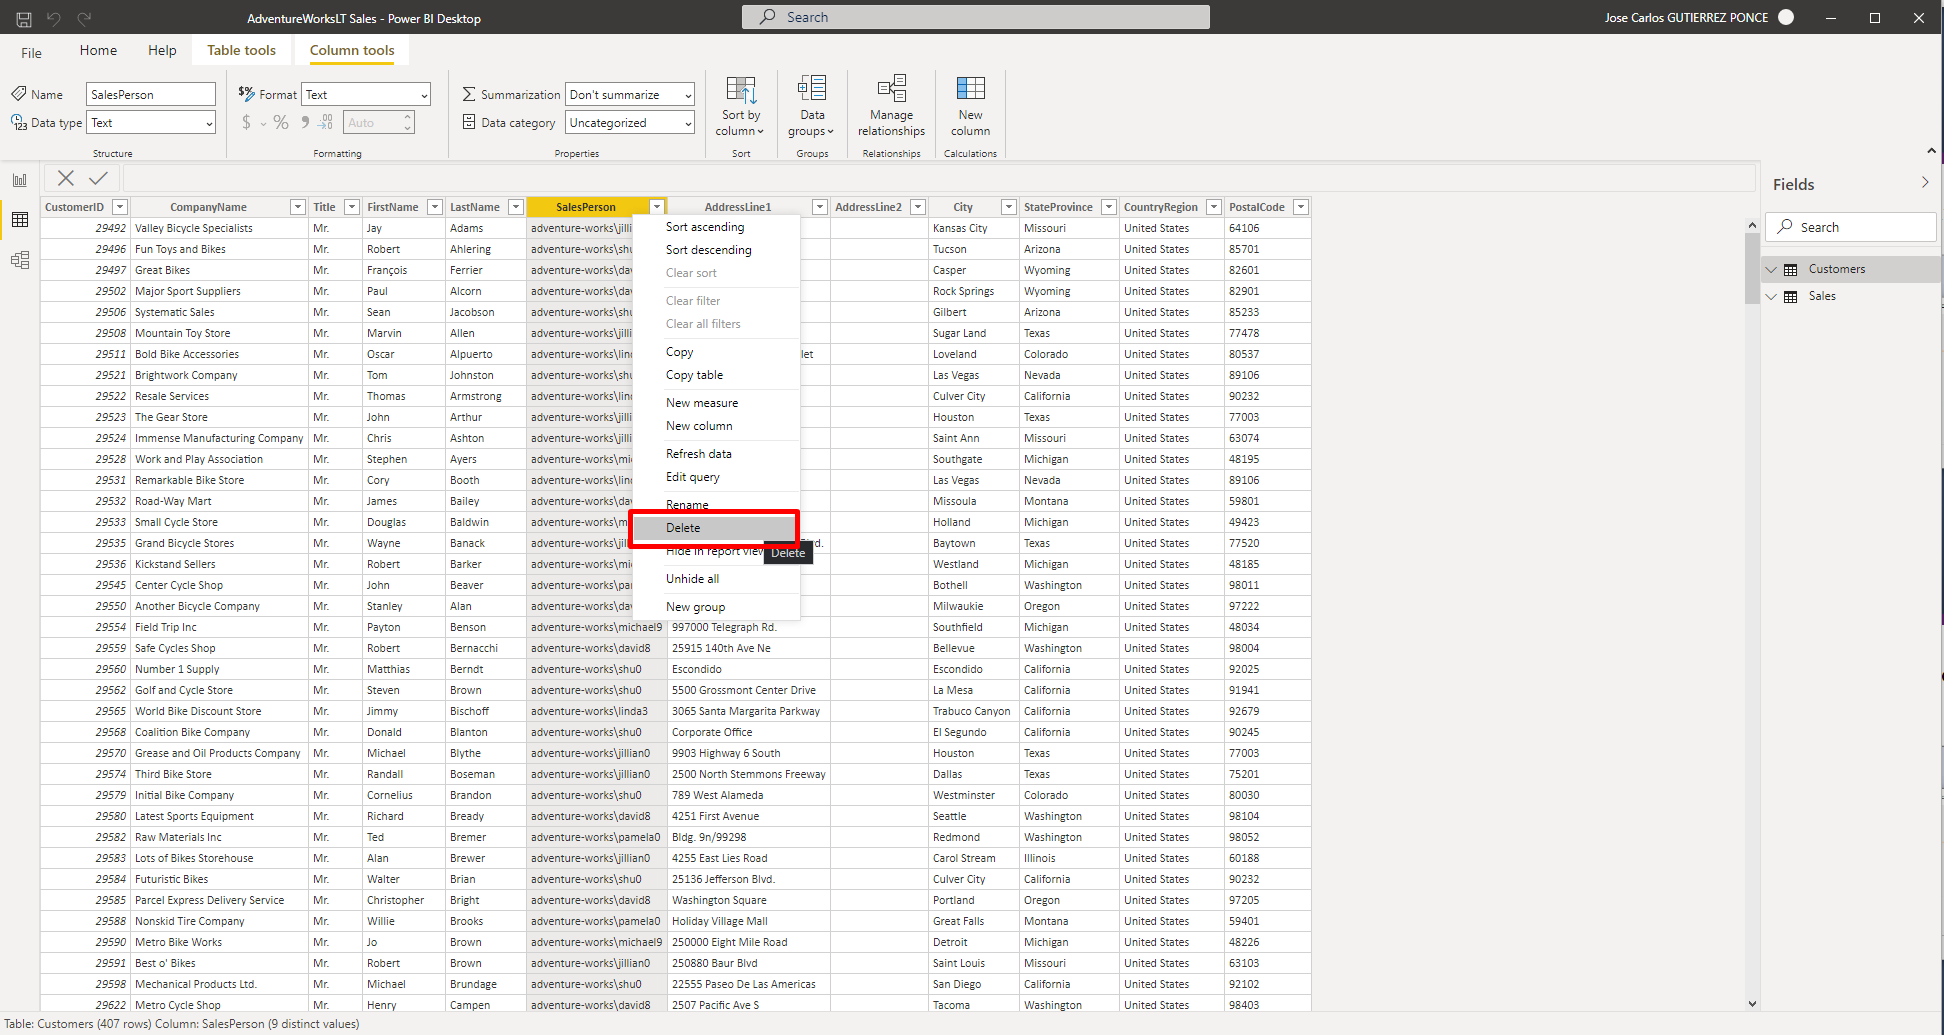
\includegraphics[width=14cm]{./images/21} 
	\end{center}
\newpage
\textbf{2.9. En el cuadro de diálogo \textbf{Delete Column}, haga clic en \textbf{Delete}.}

    \begin{center}
		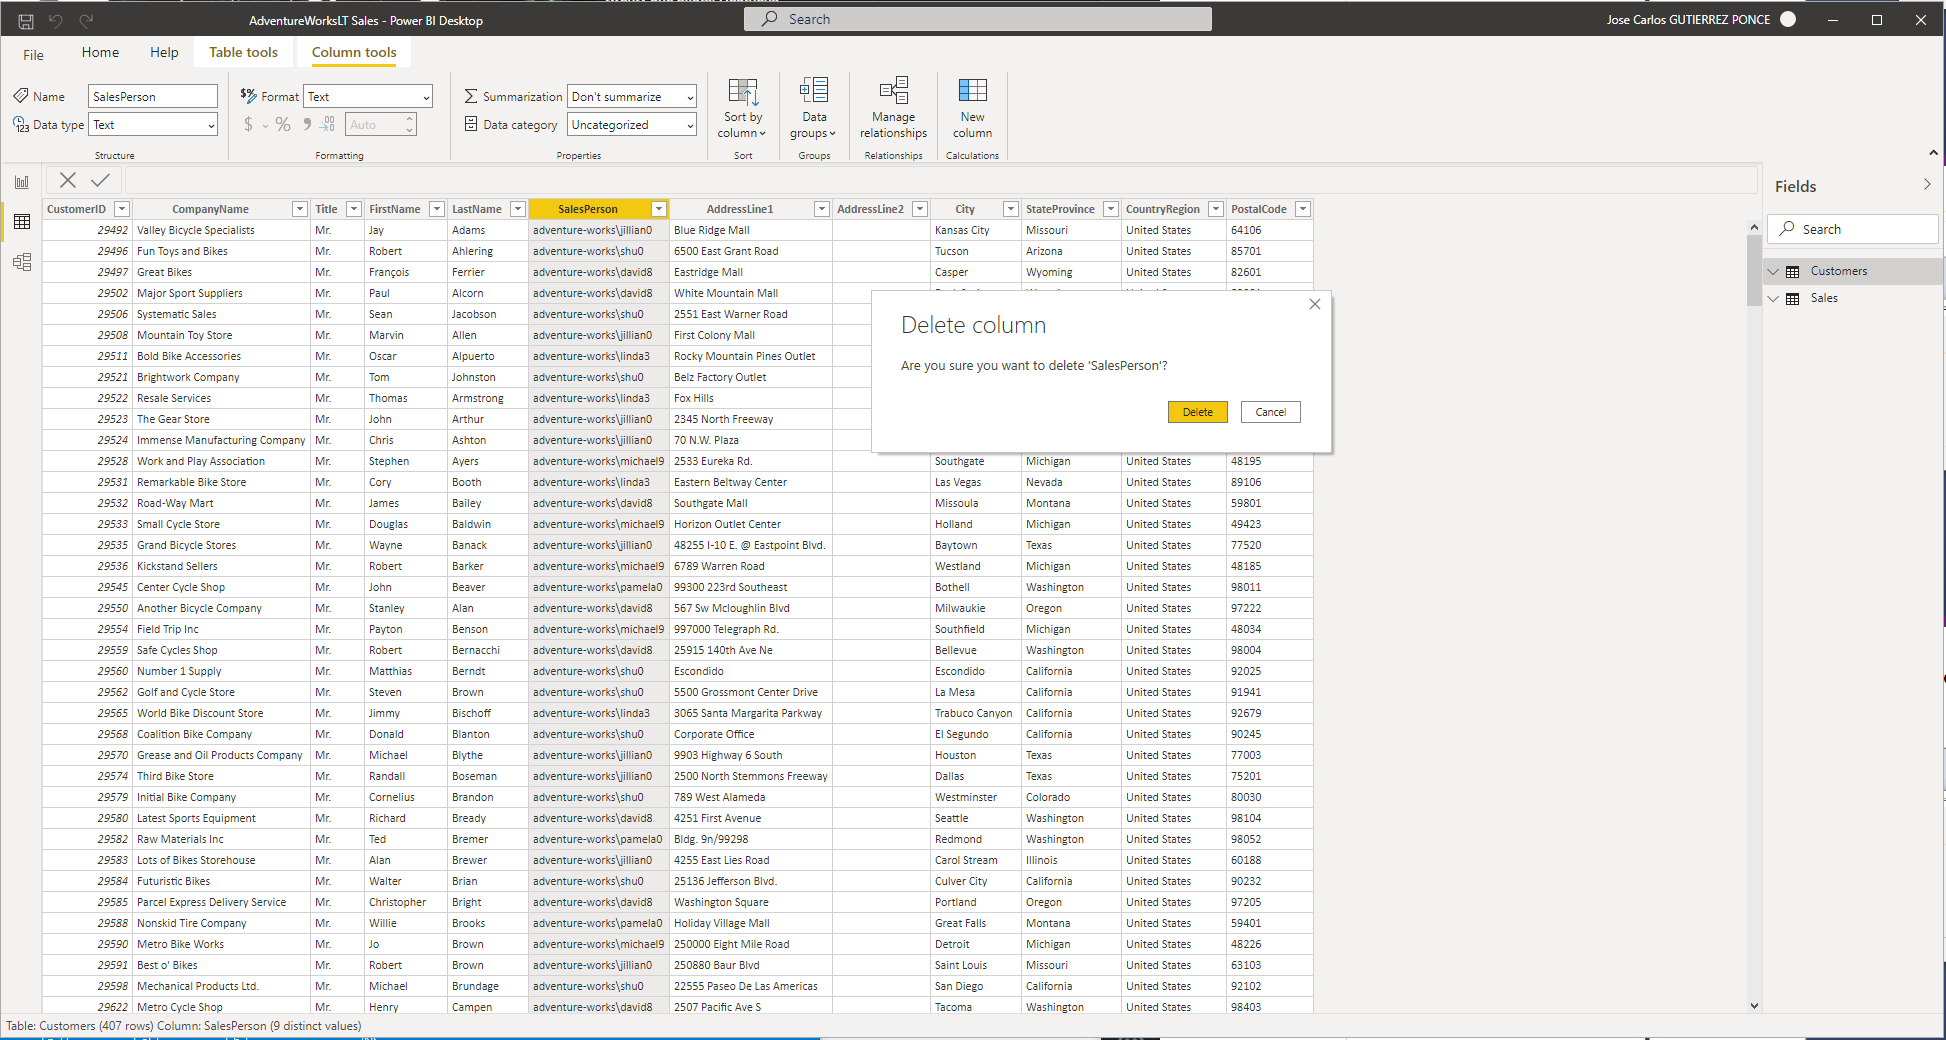
\includegraphics[width=14cm]{./images/22} 
	\end{center}
	
\textbf{2.10. Haga clic con el botón derecho en la columna \textbf{CustomerID} y luego haga clic en \textbf{Hide in ReportView}.}

    \begin{center}
		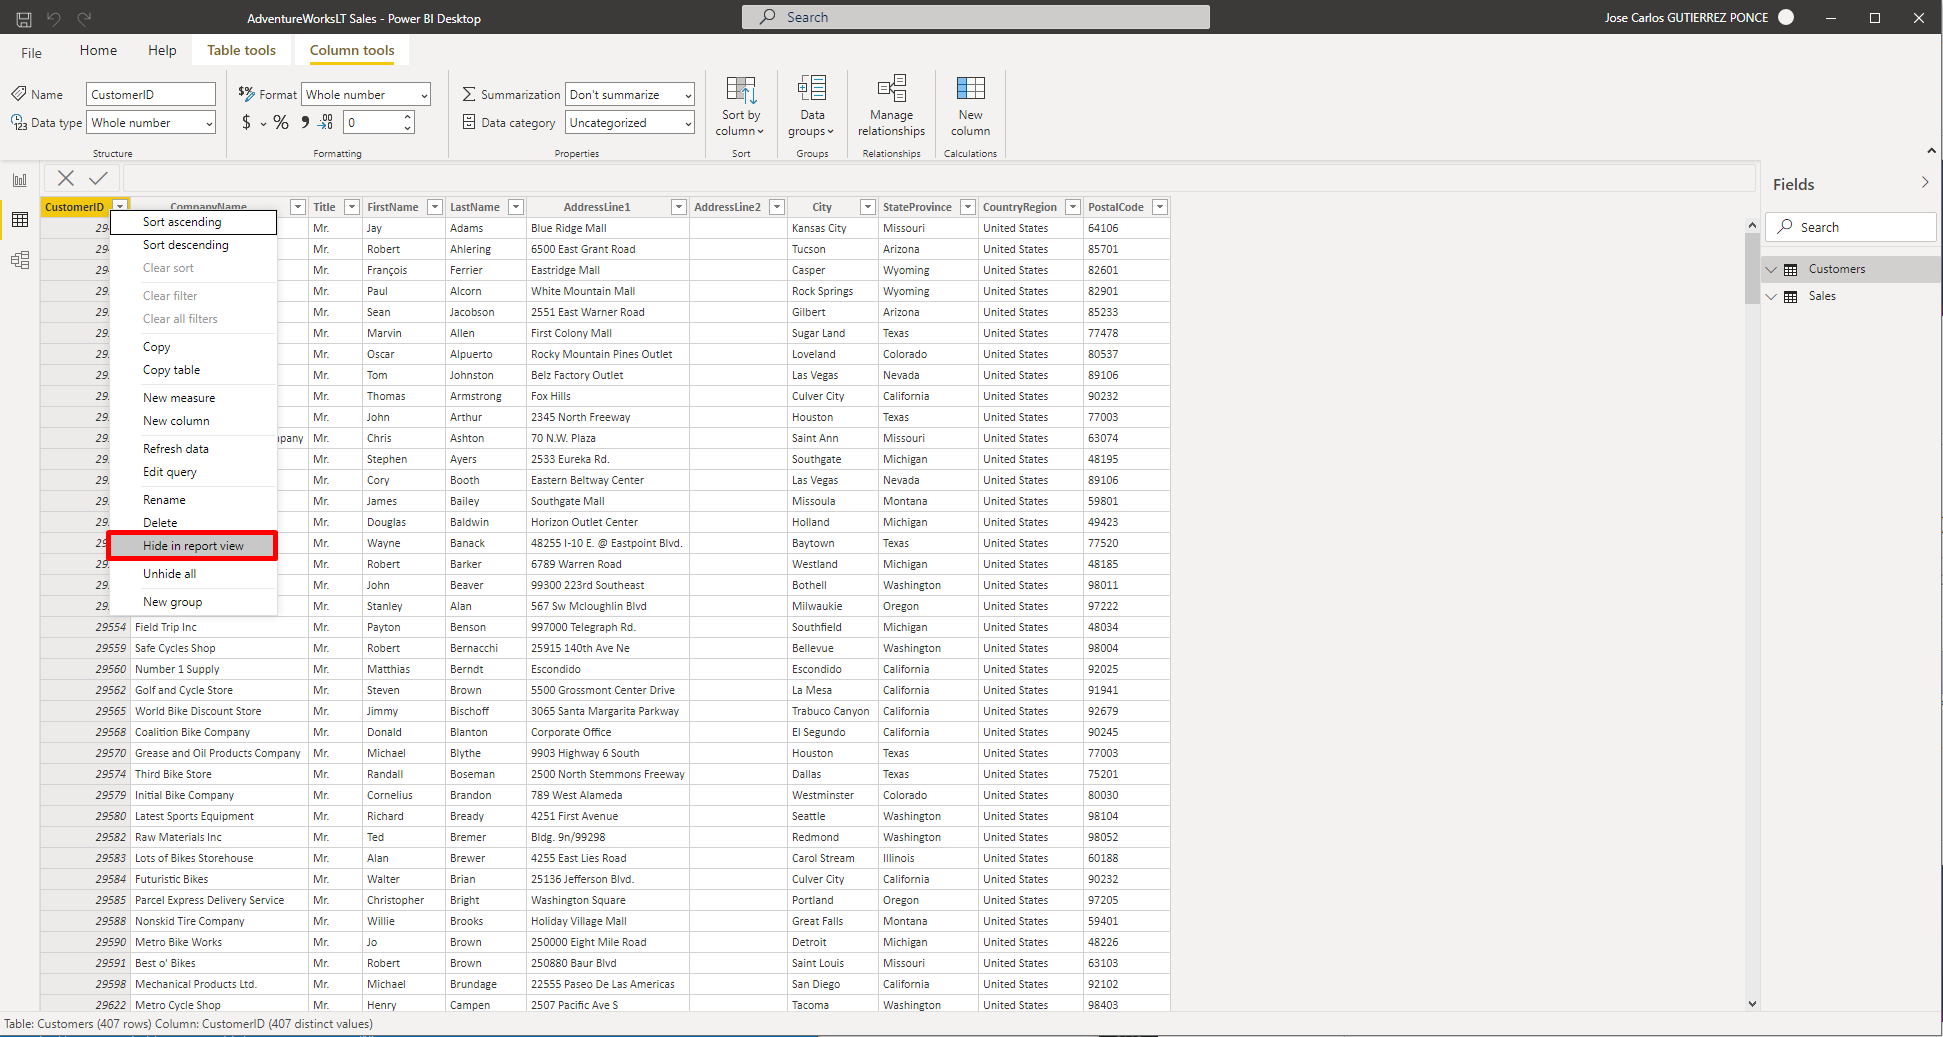
\includegraphics[width=14cm]{./images/23} 
	\end{center}
\newpage	
\textbf{2.11. Haga clic en el encabezado de la columna \textbf{AddressLine1}.}

    \begin{center}
		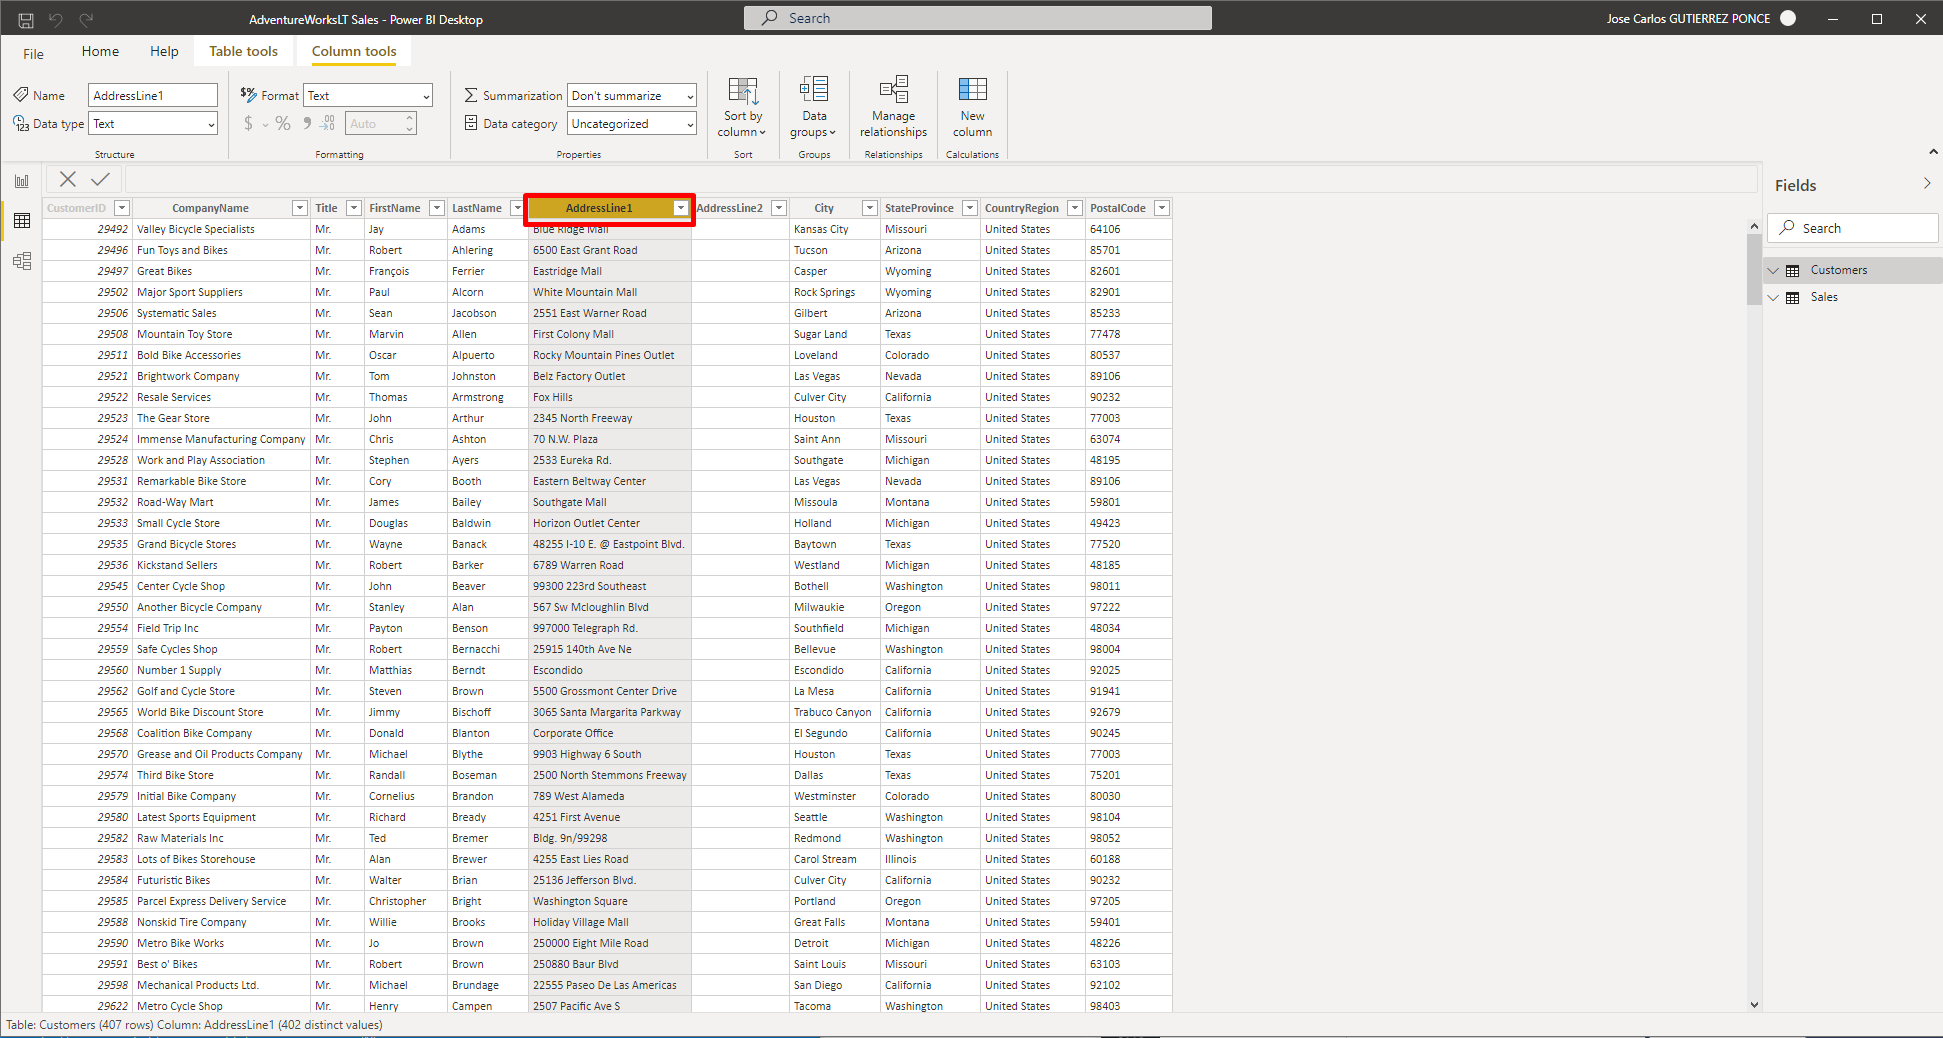
\includegraphics[width=14cm]{./images/24} 
	\end{center}
	
\textbf{2.12. En la cinta \textbf{Modeling}, en el grupo \textbf{Properties}, haga clic en \textbf{DataCategory: Uncategorized} y luego en \textbf{Address}.}

    \begin{center}
		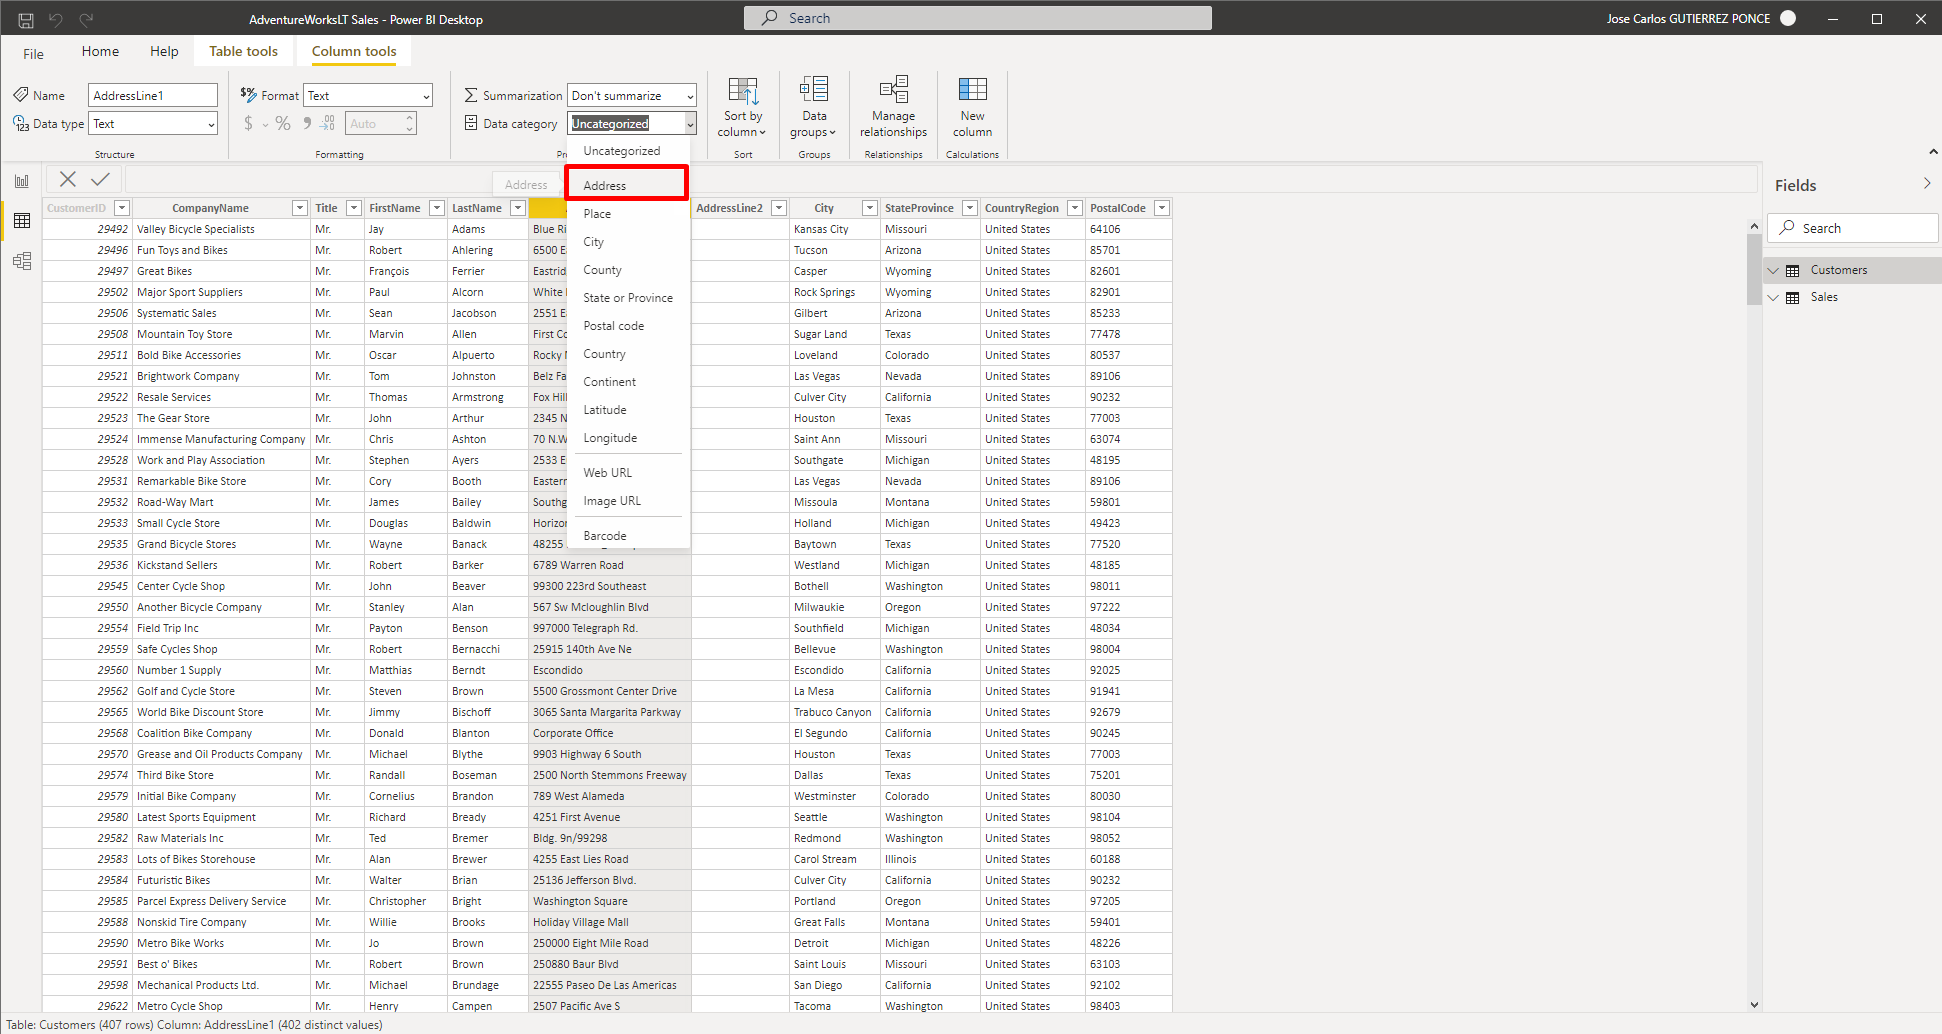
\includegraphics[width=14cm]{./images/25} 
	\end{center}
\newpage	
\textbf{2.13. Haga clic en el encabezado de la columna \textbf{City}.}

    \begin{center}
		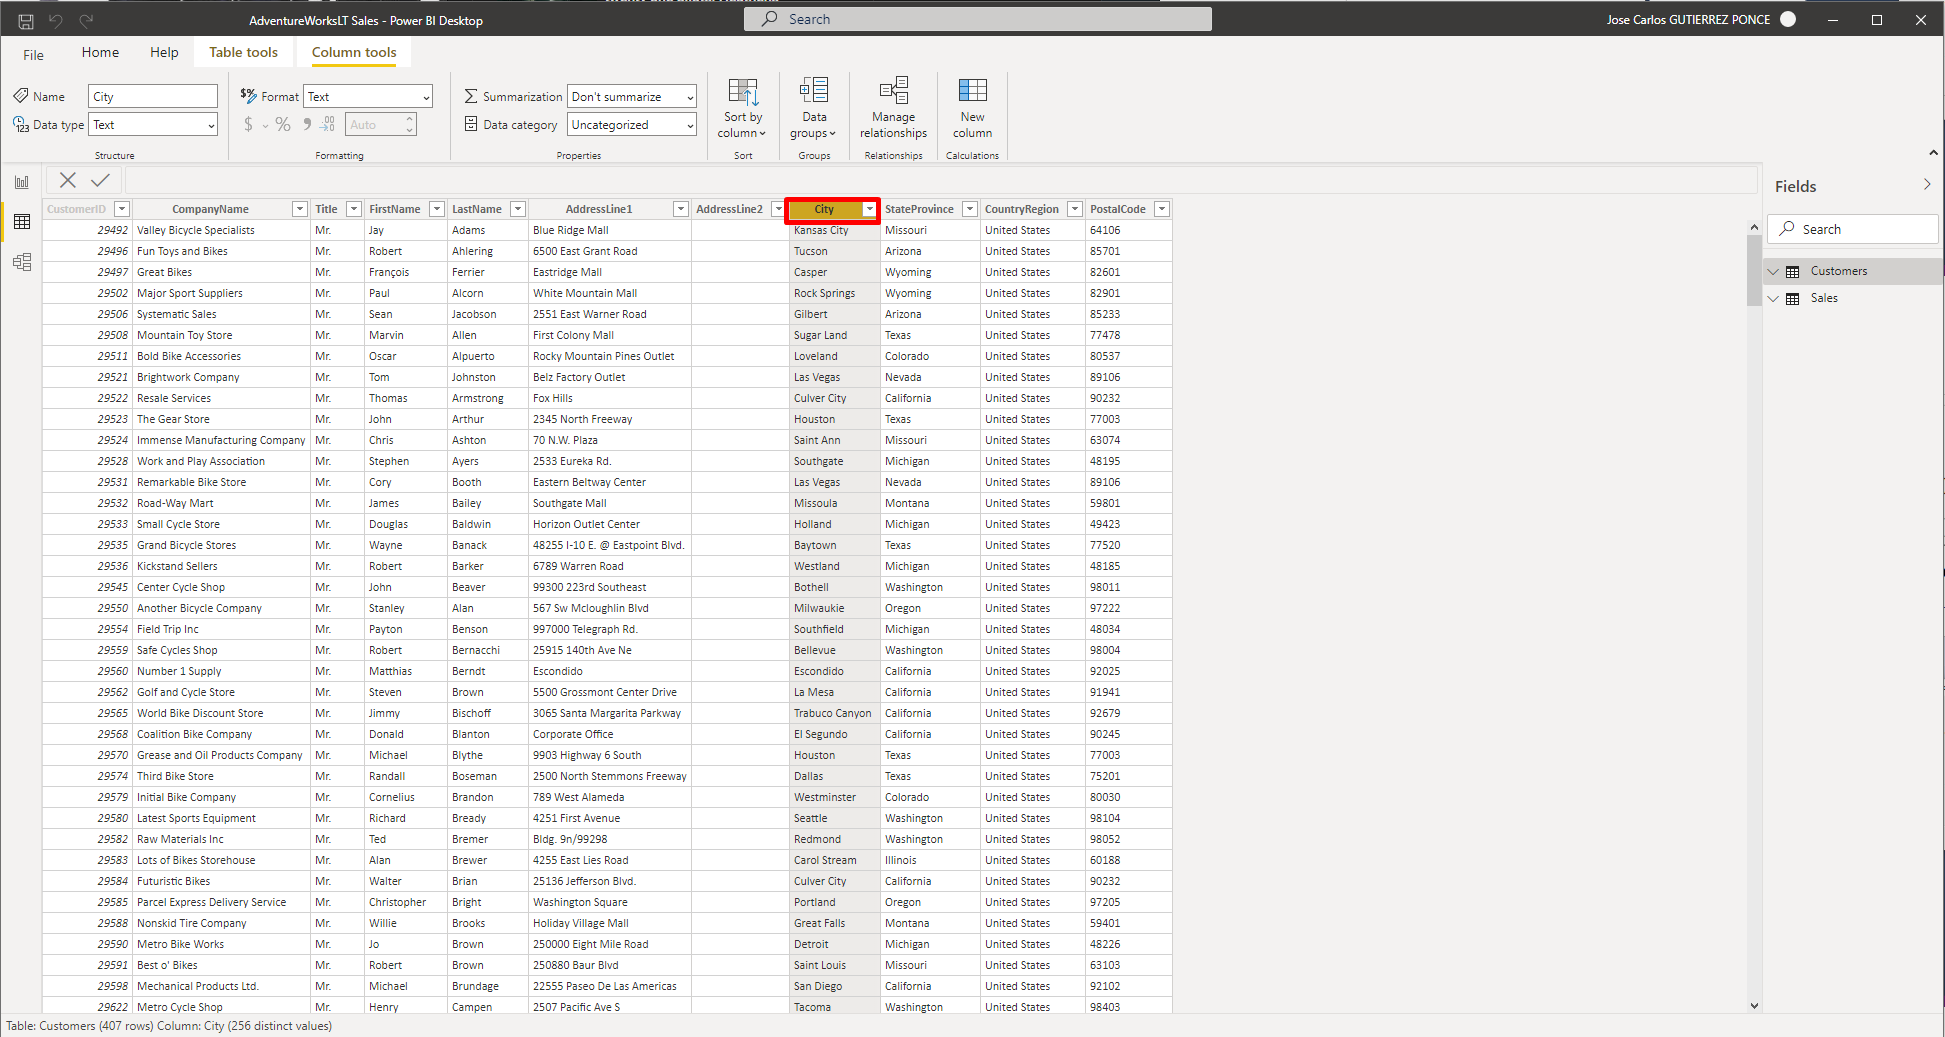
\includegraphics[width=14cm]{./images/26} 
	\end{center}
	
\textbf{2.14. En la cinta de \textbf{Modeling}, en el grupo \textbf{Properties}, haga clic en \textbf{DataCategory: Uncategorized} y, a continuación, haga clic en \textbf{City}.}

    \begin{center}
		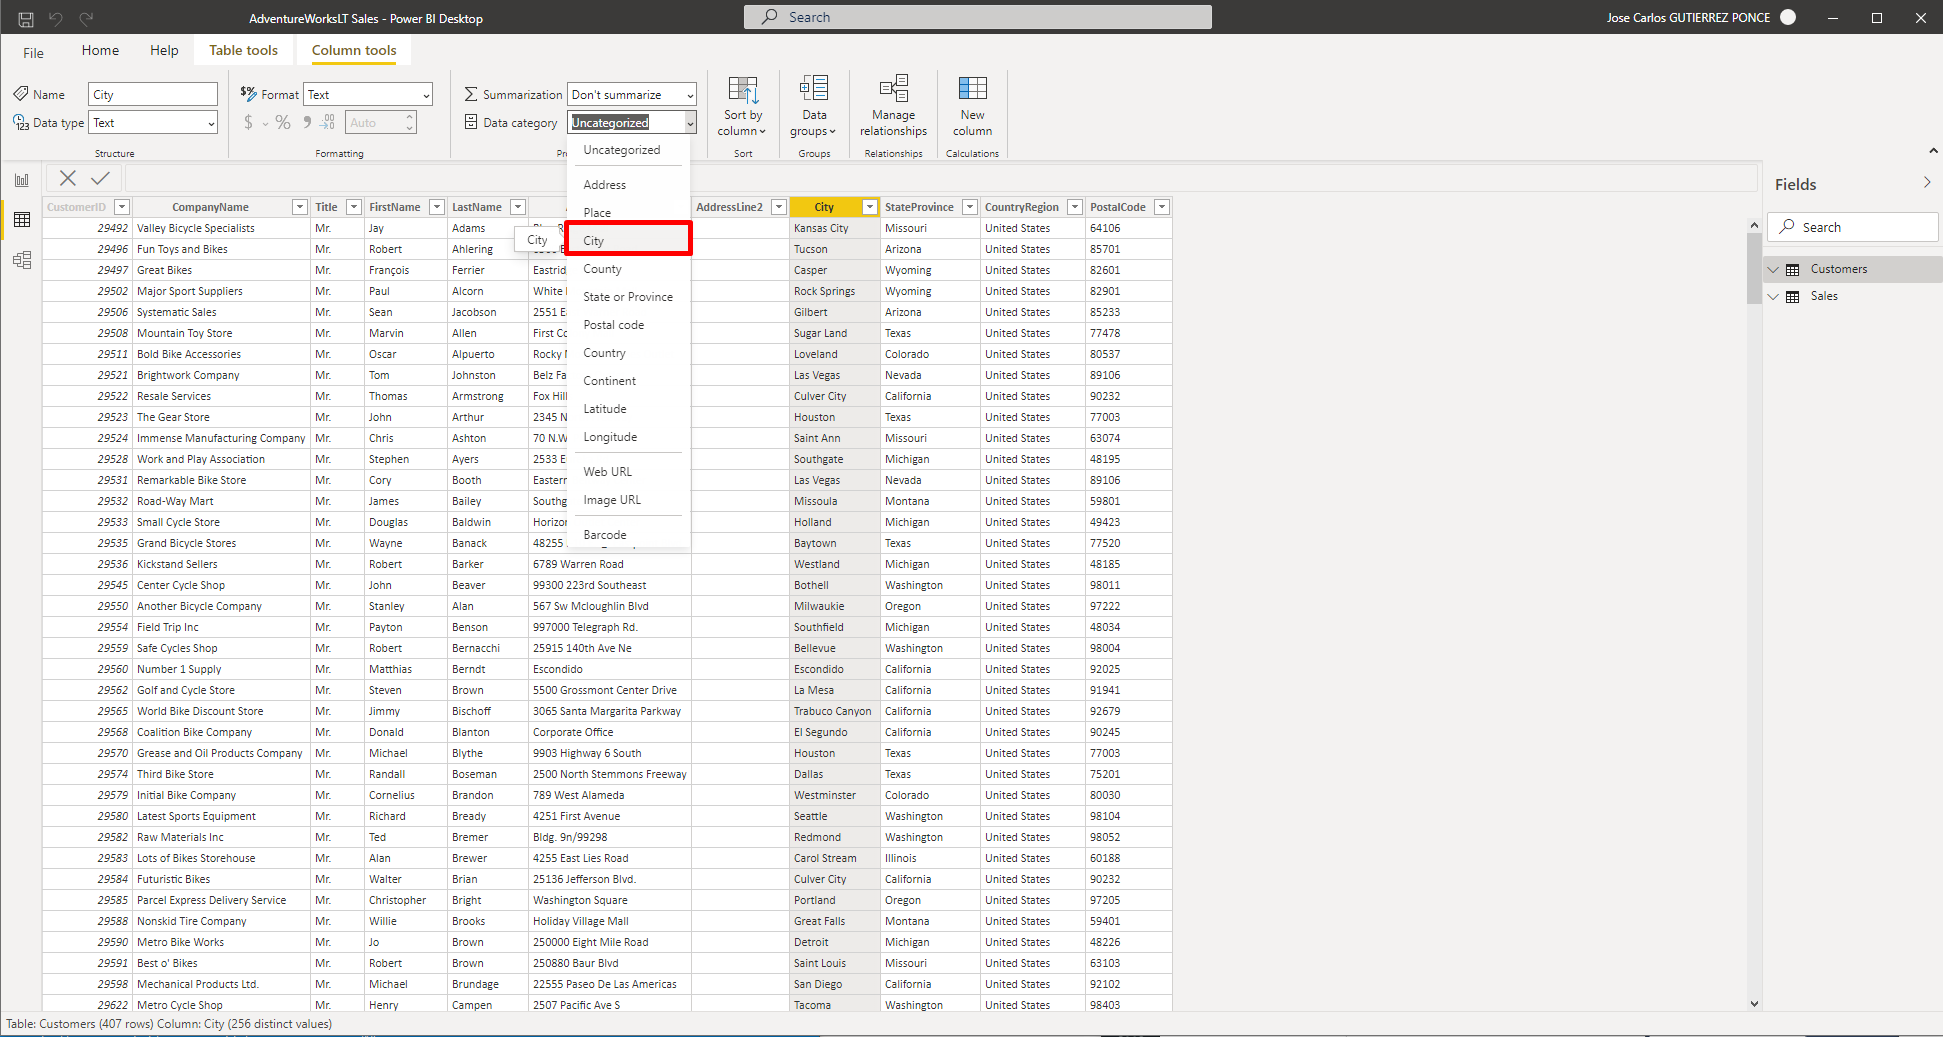
\includegraphics[width=14cm]{./images/27} 
	\end{center}
\newpage	
\textbf{2.15 Haga clic en el encabezado de la columna \textbf{StateProvince}.}

    \begin{center}
		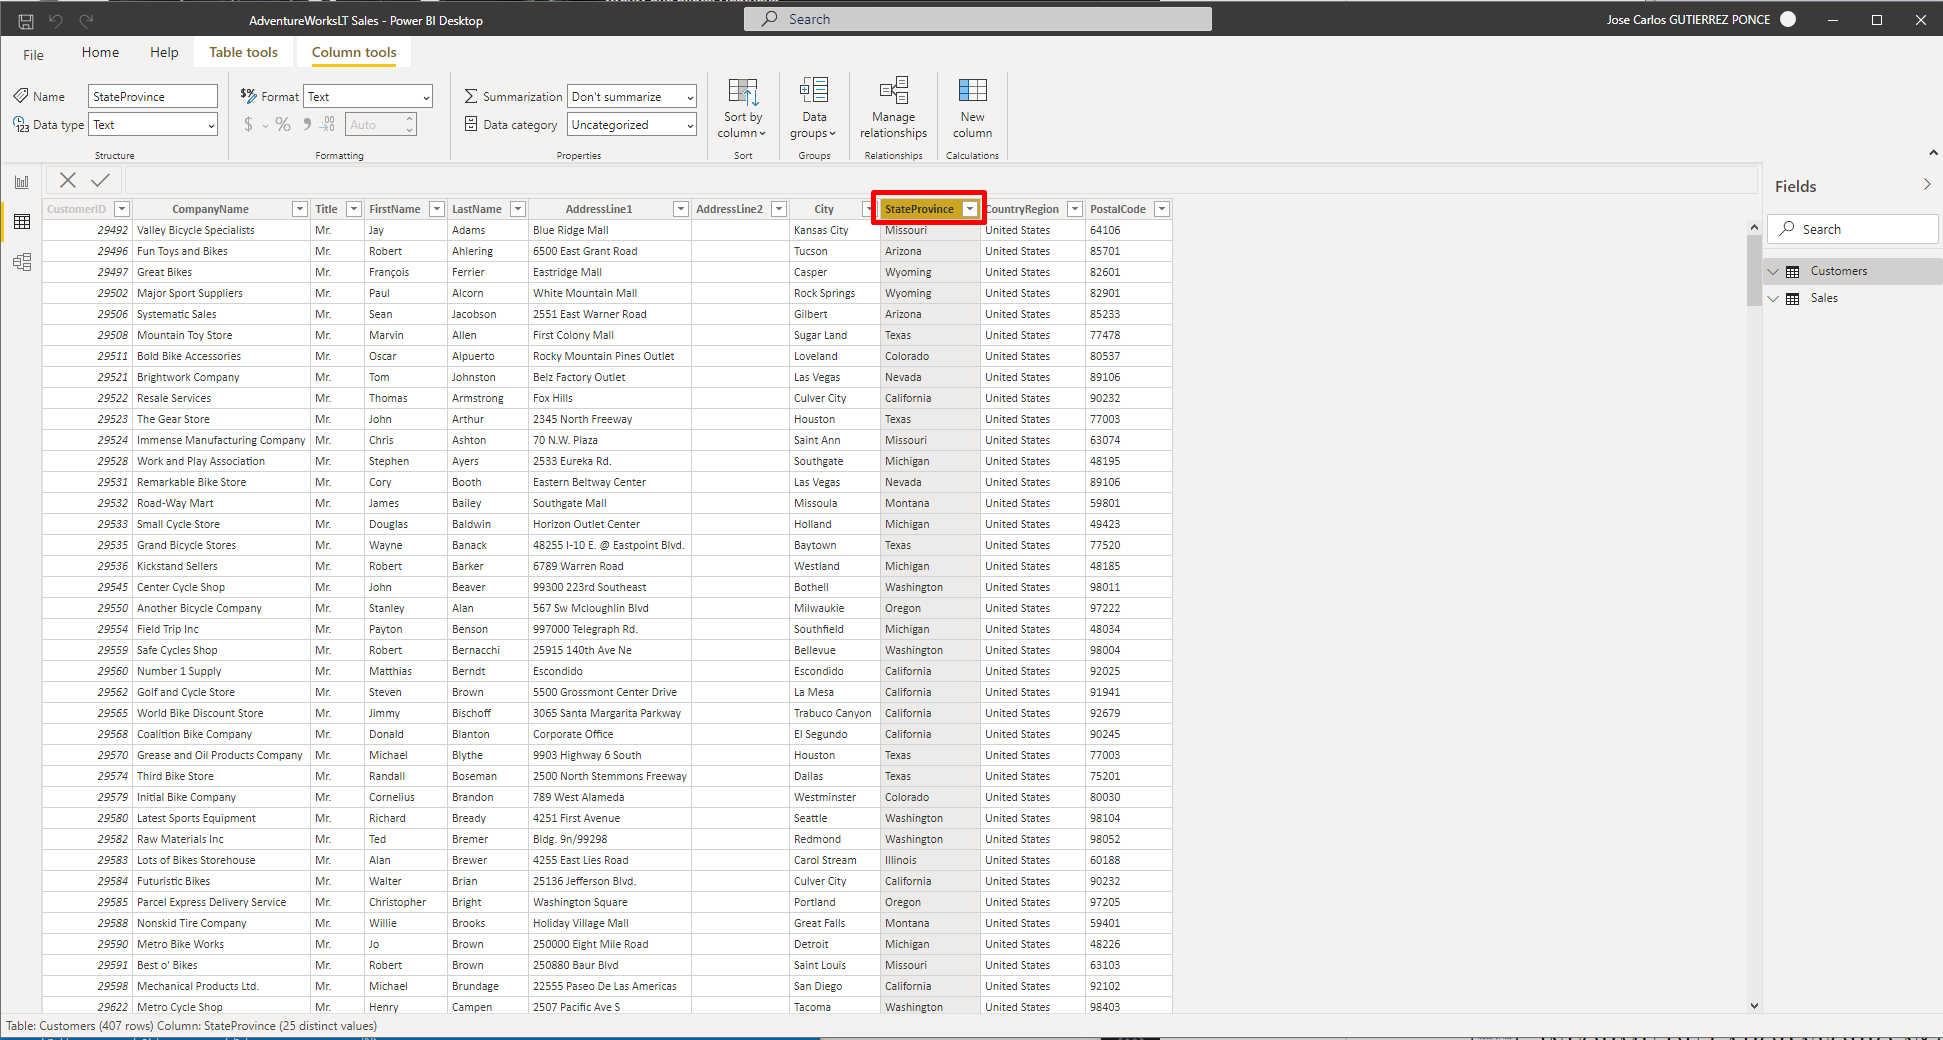
\includegraphics[width=14cm]{./images/28} 
	\end{center}
	
\textbf{2.16. En la cinta \textbf{Modeling}, en el grupo \textbf{Properties}, haga clic en \textbf{DataCategory: Uncategorized} y luego haga clic en \textbf{State or Province}.}

    \begin{center}
		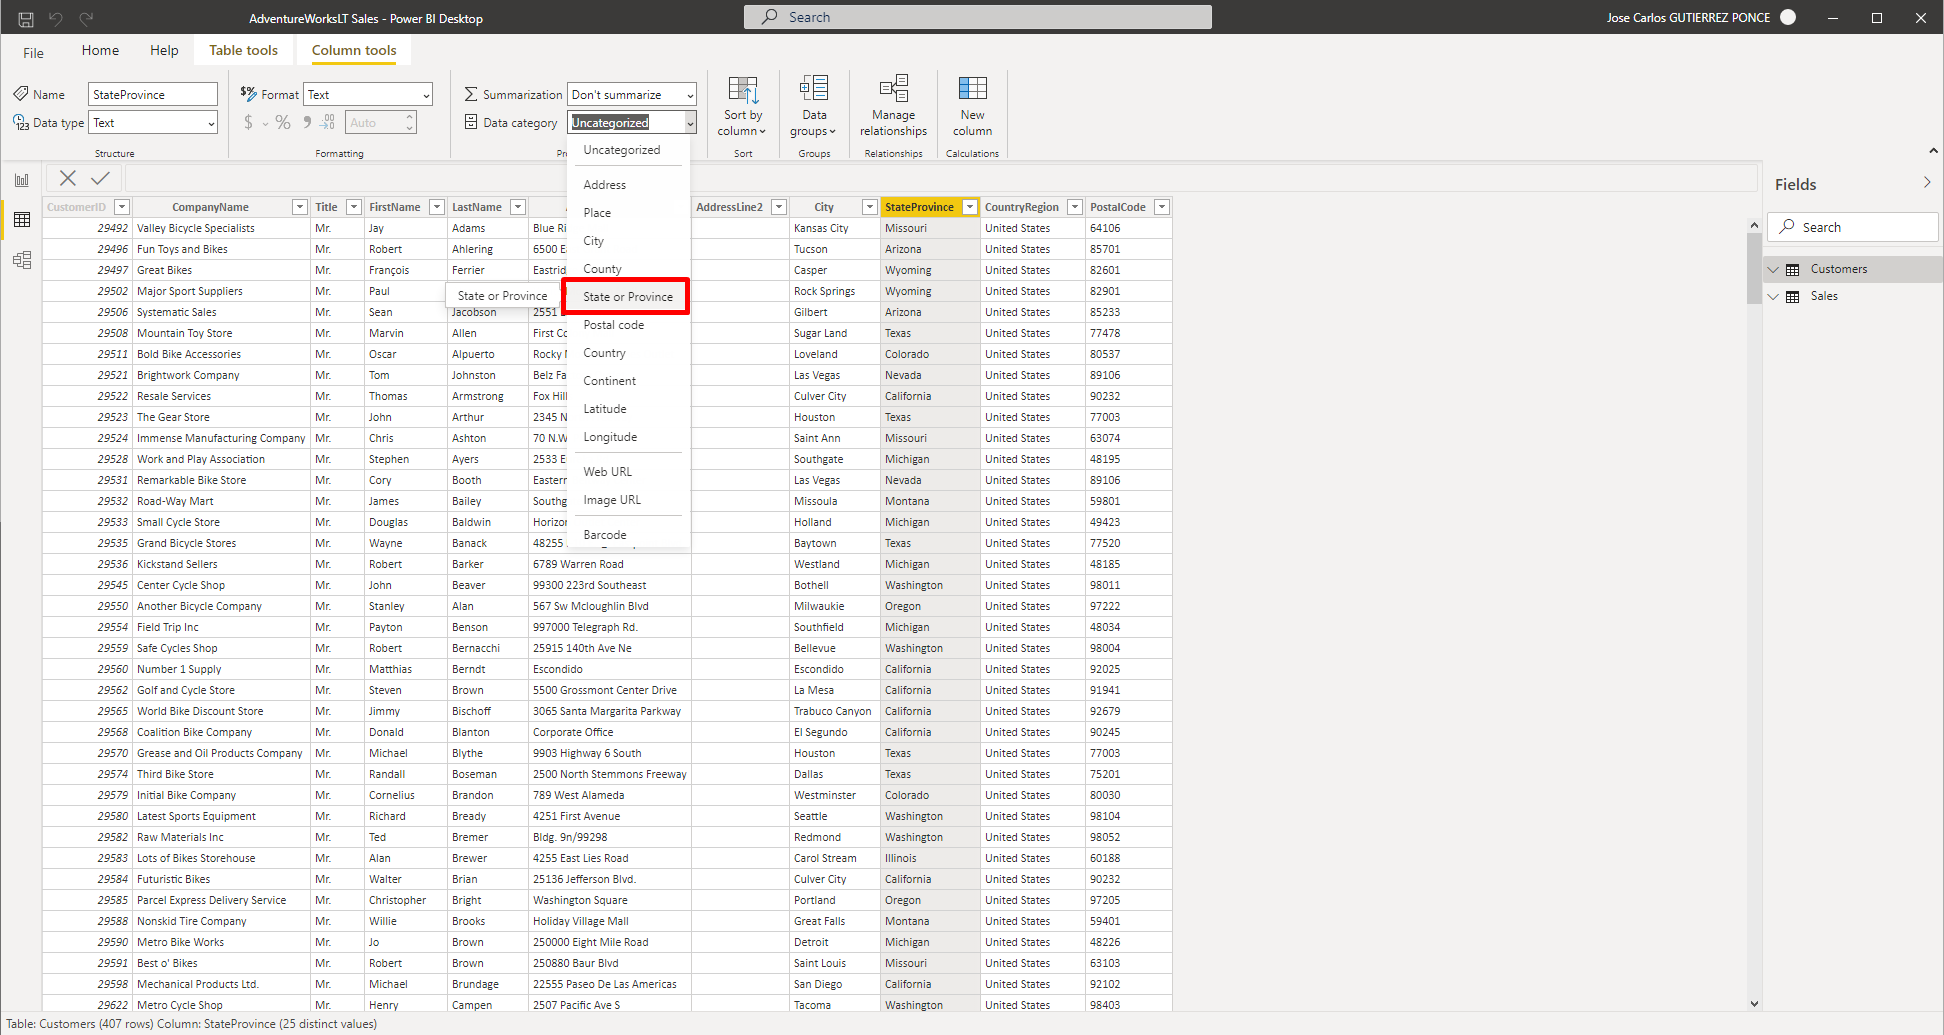
\includegraphics[width=14cm]{./images/29} 
	\end{center}
\newpage	
\textbf{2.17. Haga clic en el encabezado de la columna \textbf{CountryRegion}.}

    \begin{center}
		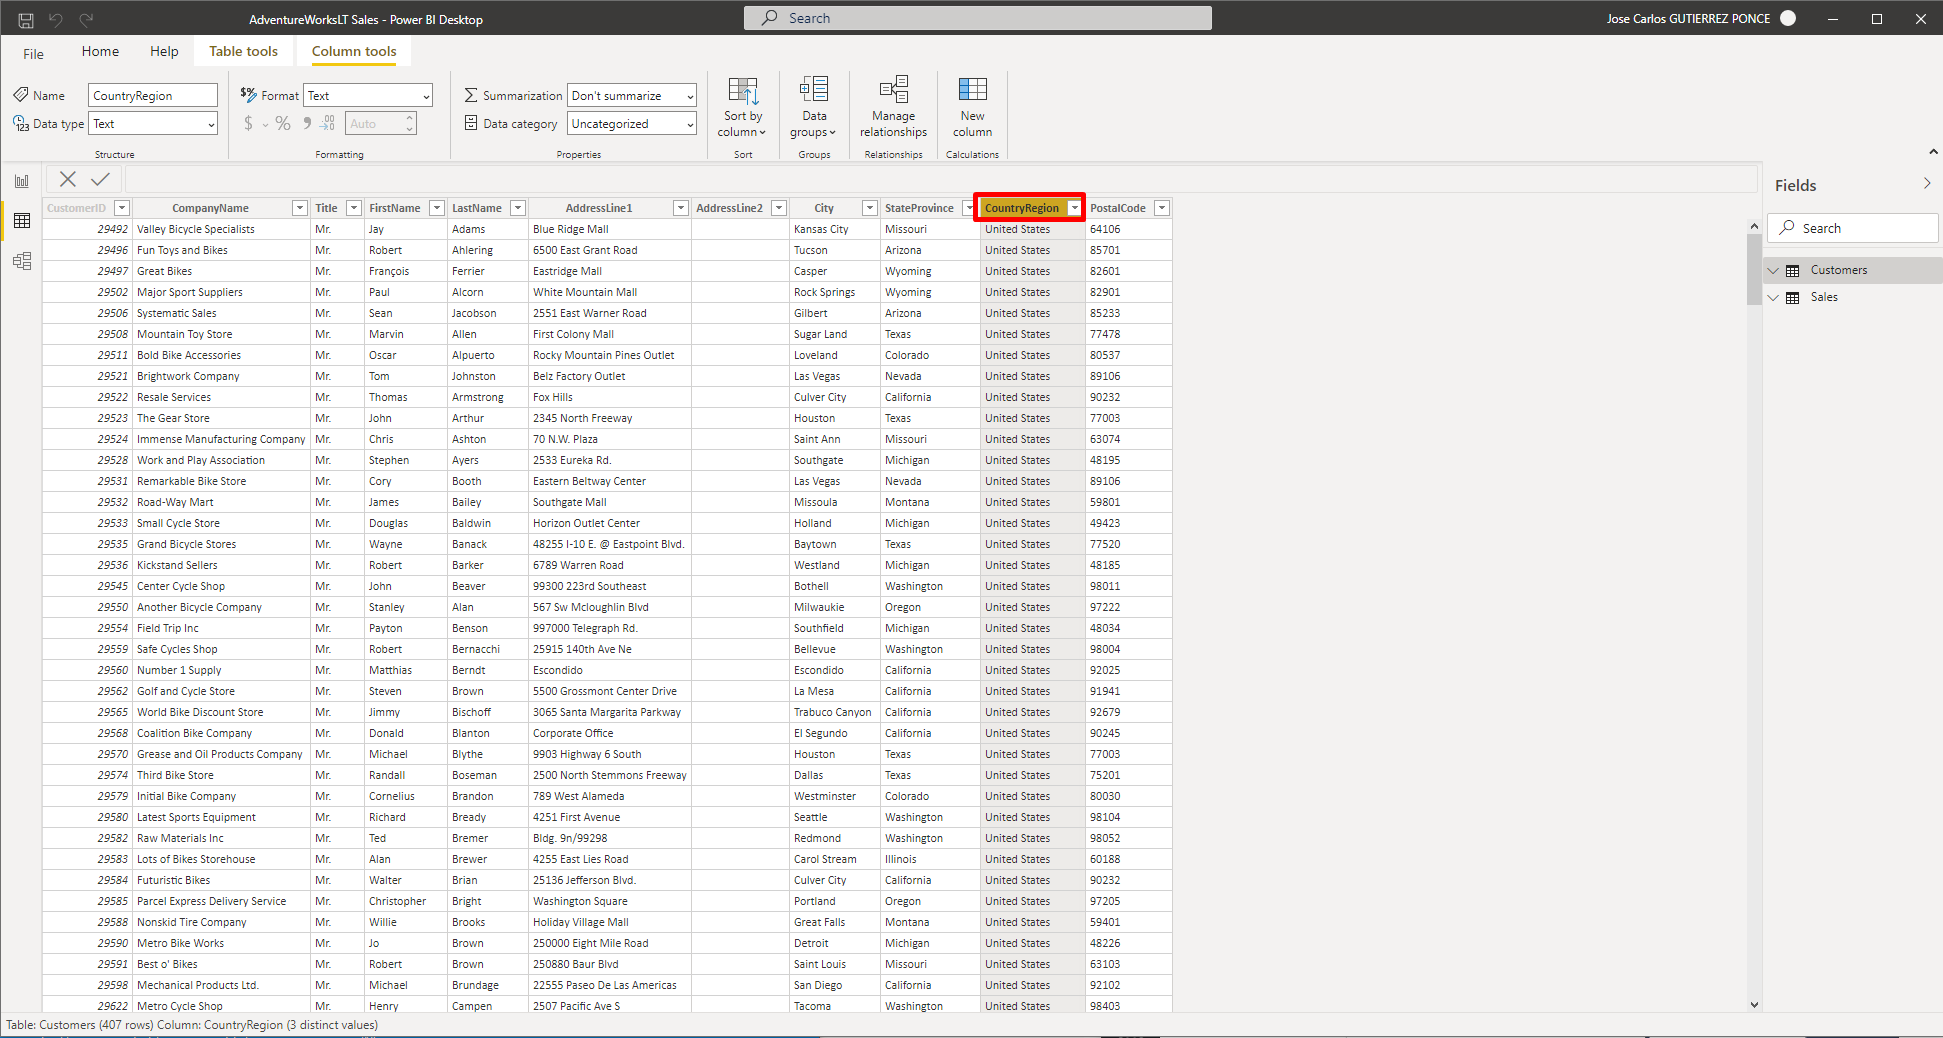
\includegraphics[width=14cm]{./images/30} 
	\end{center}
	
\textbf{2.18. En la cinta \textbf{Modeling}, en el grupo \textbf{Properties}, haga clic en \textbf{DataCategory: Uncategorized} y luego haga clic en \textbf{Country}.}

    \begin{center}
		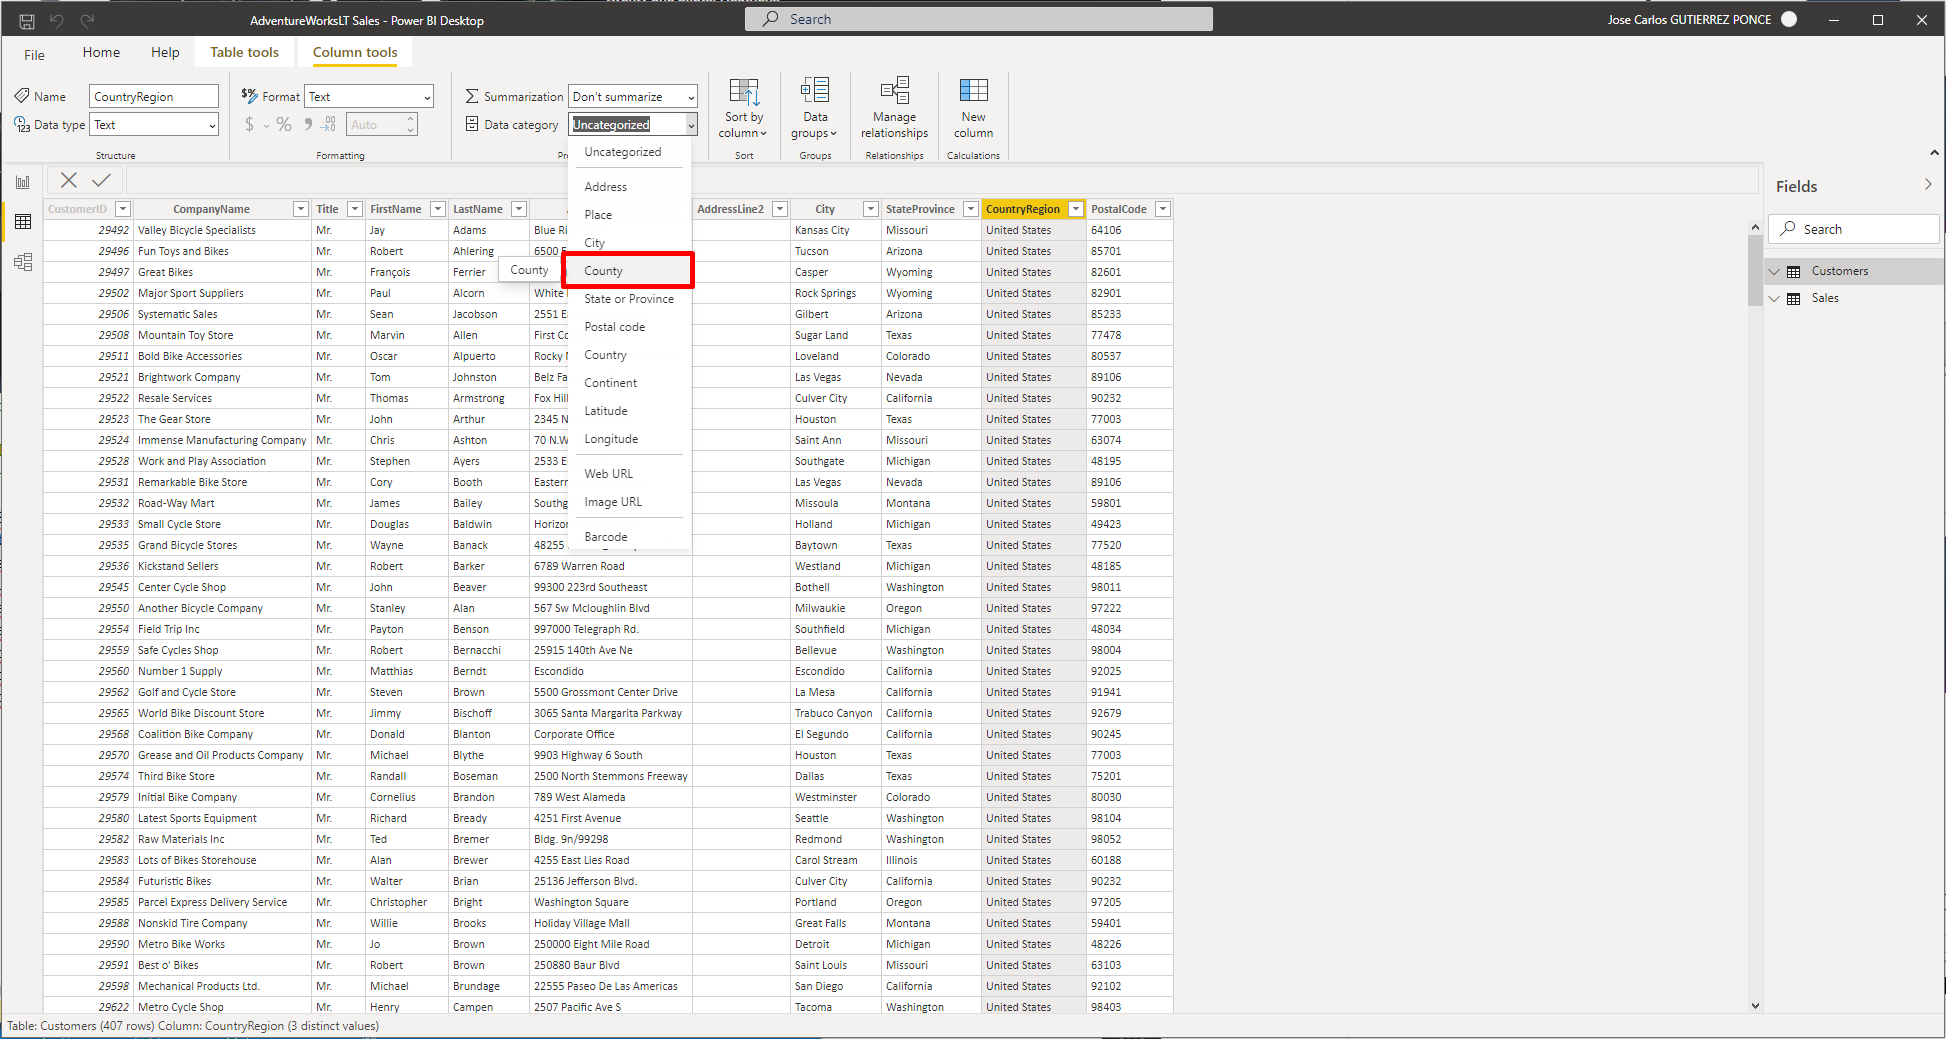
\includegraphics[width=14cm]{./images/31} 
	\end{center}
\newpage	
\textbf{2.19. Haga clic en el encabezado de la columna \textbf{PostalCode}.}

    \begin{center}
		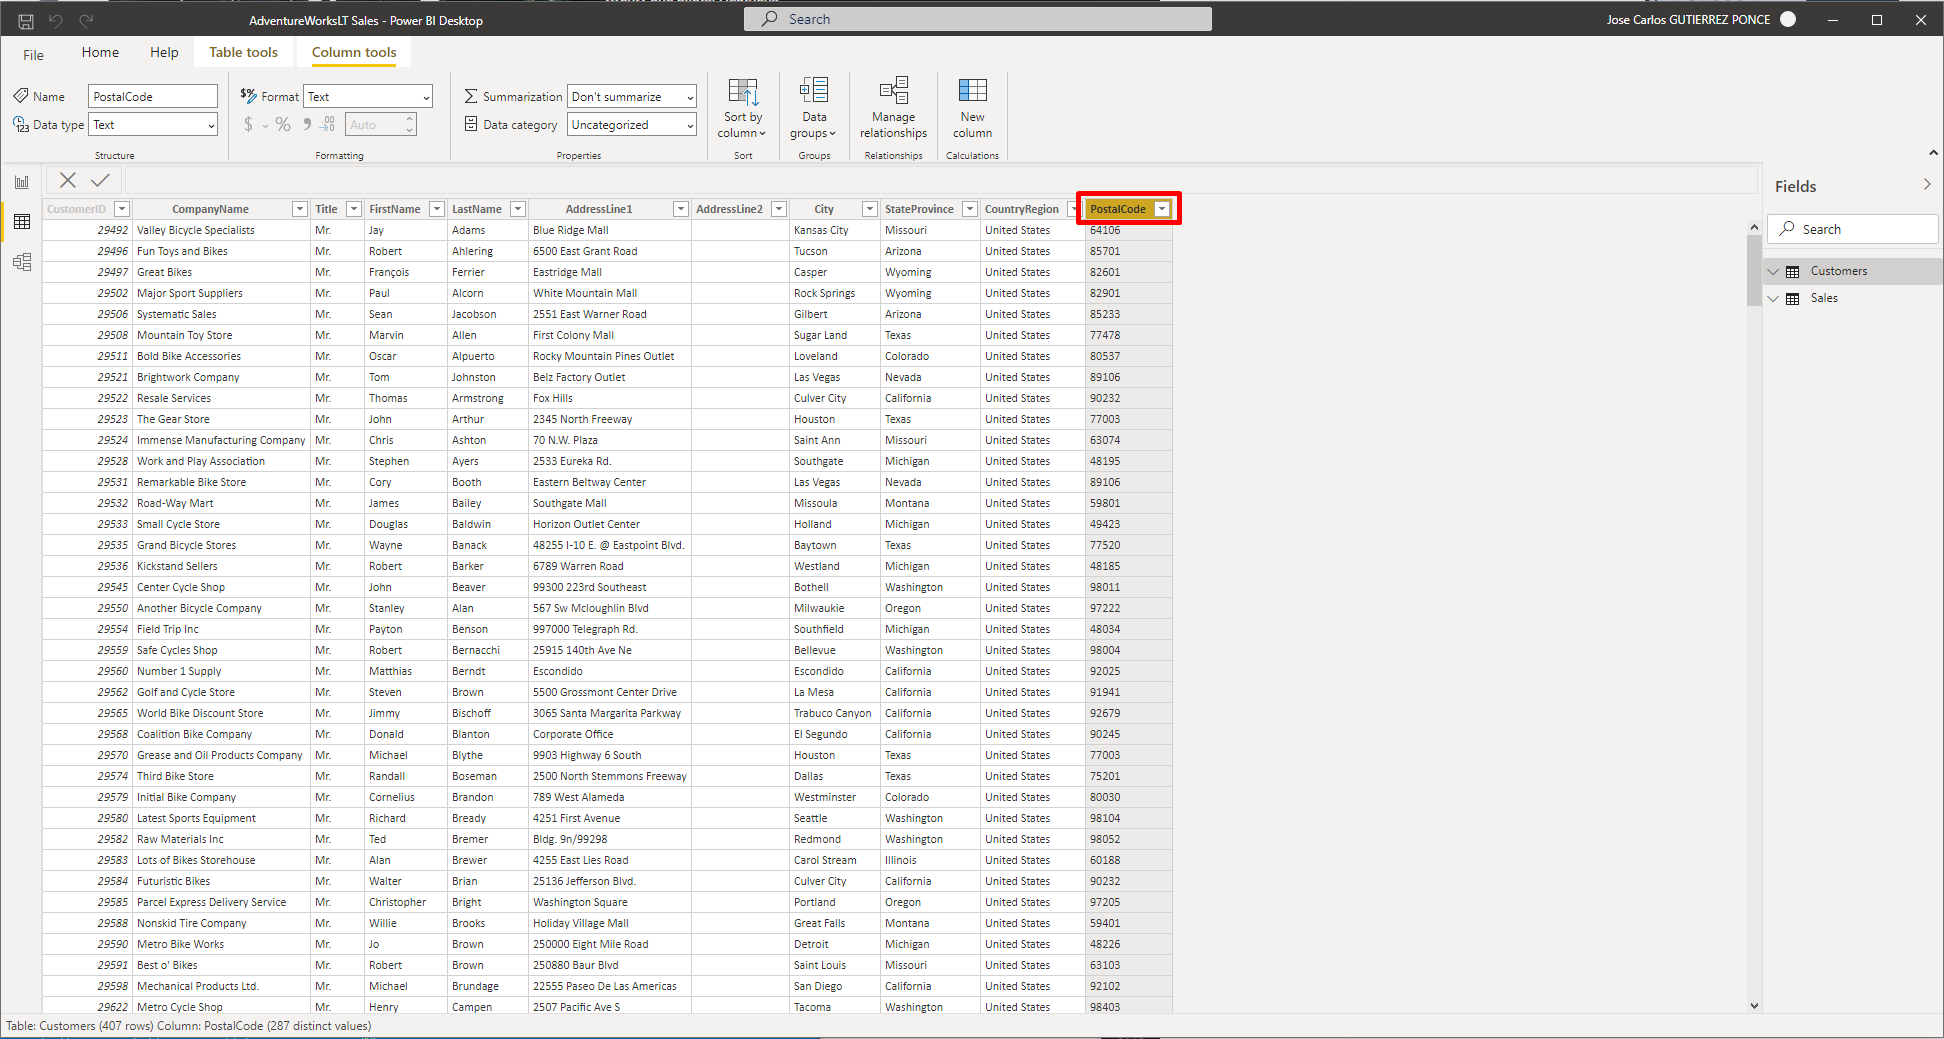
\includegraphics[width=14cm]{./images/32} 
	\end{center}
	
\textbf{2.20. En la cinta \textbf{Modeling}, en el grupo \textbf{Properties}, haga clic en \textbf{DataCategory: Uncategorized} y luego en \textbf{Postal Code}.}

    \begin{center}
		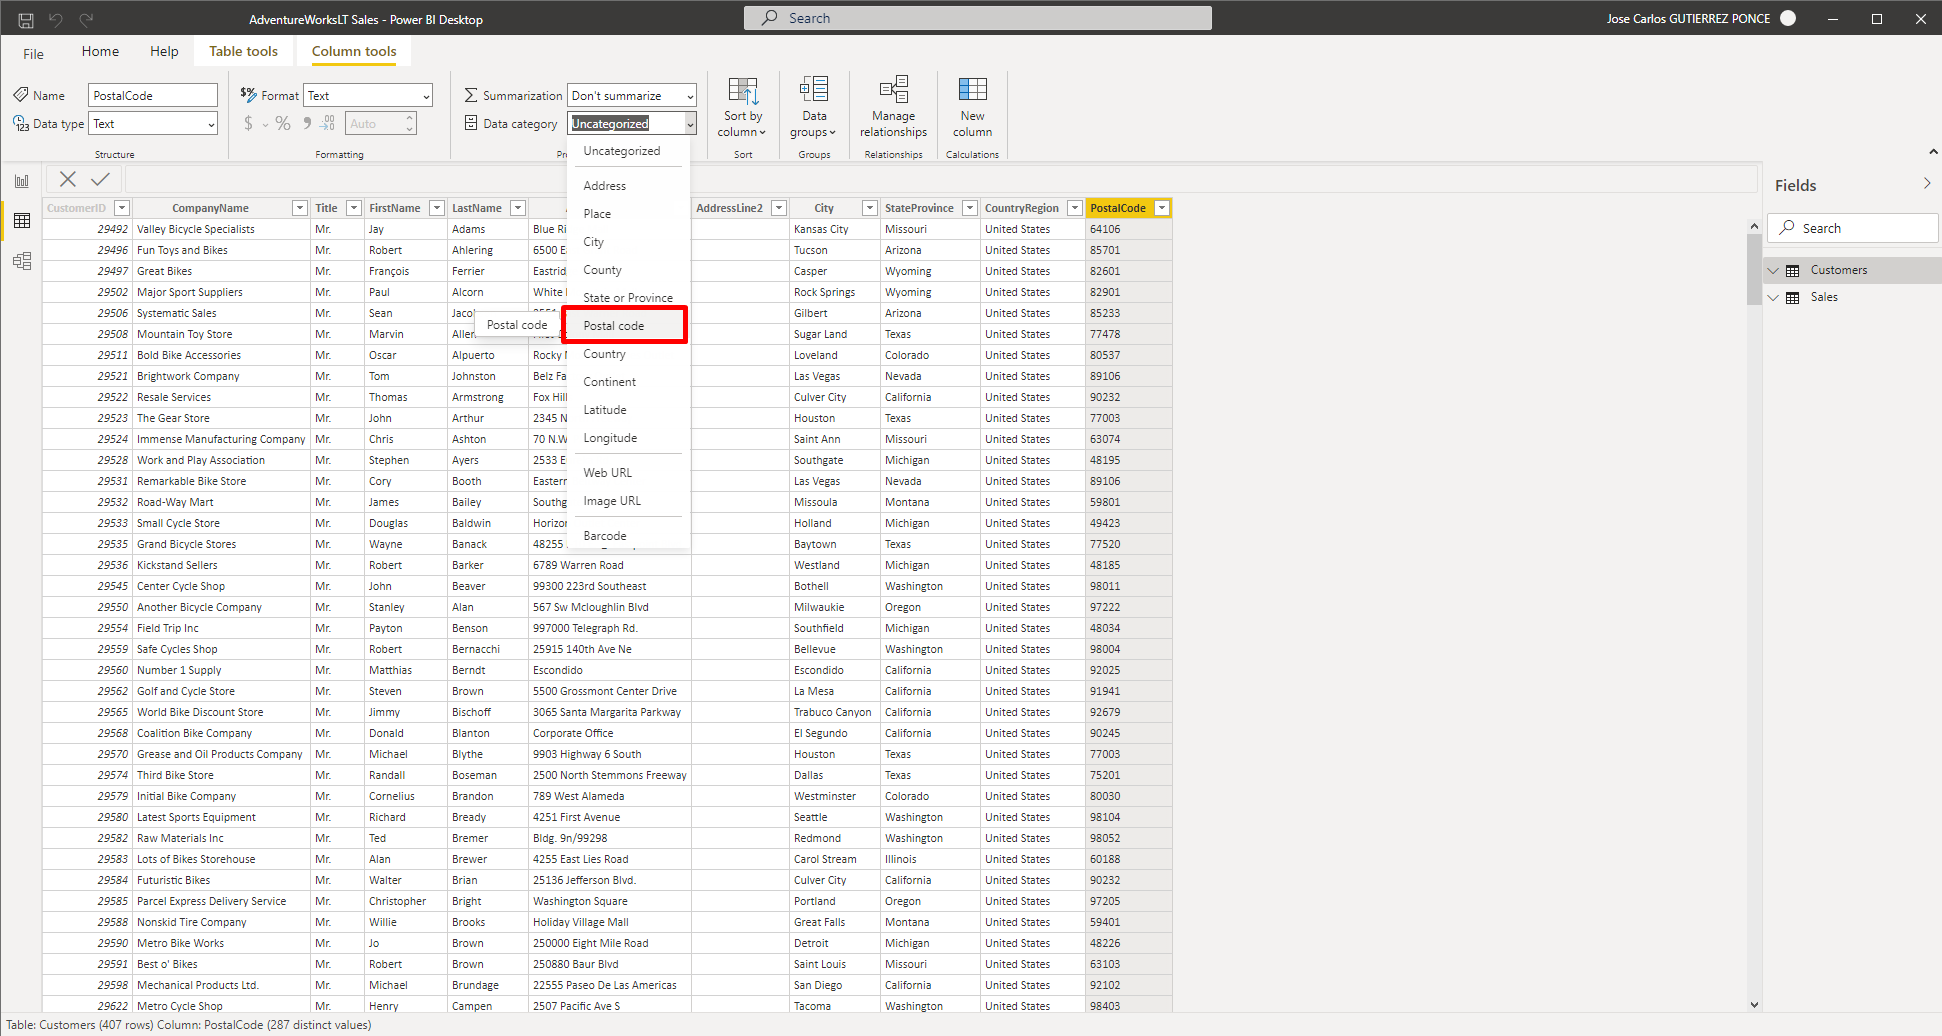
\includegraphics[width=14cm]{./images/33} 
	\end{center}
\newpage	
\textbf{2.21. En la cinta \textbf{Modeling}, en el grupo \textbf{Calculations}, haga clic en \textbf{NewColumn} y luego en la barra de fórmulas, escriba la siguiente expresión y presione Enter:}

    \begin{center}
		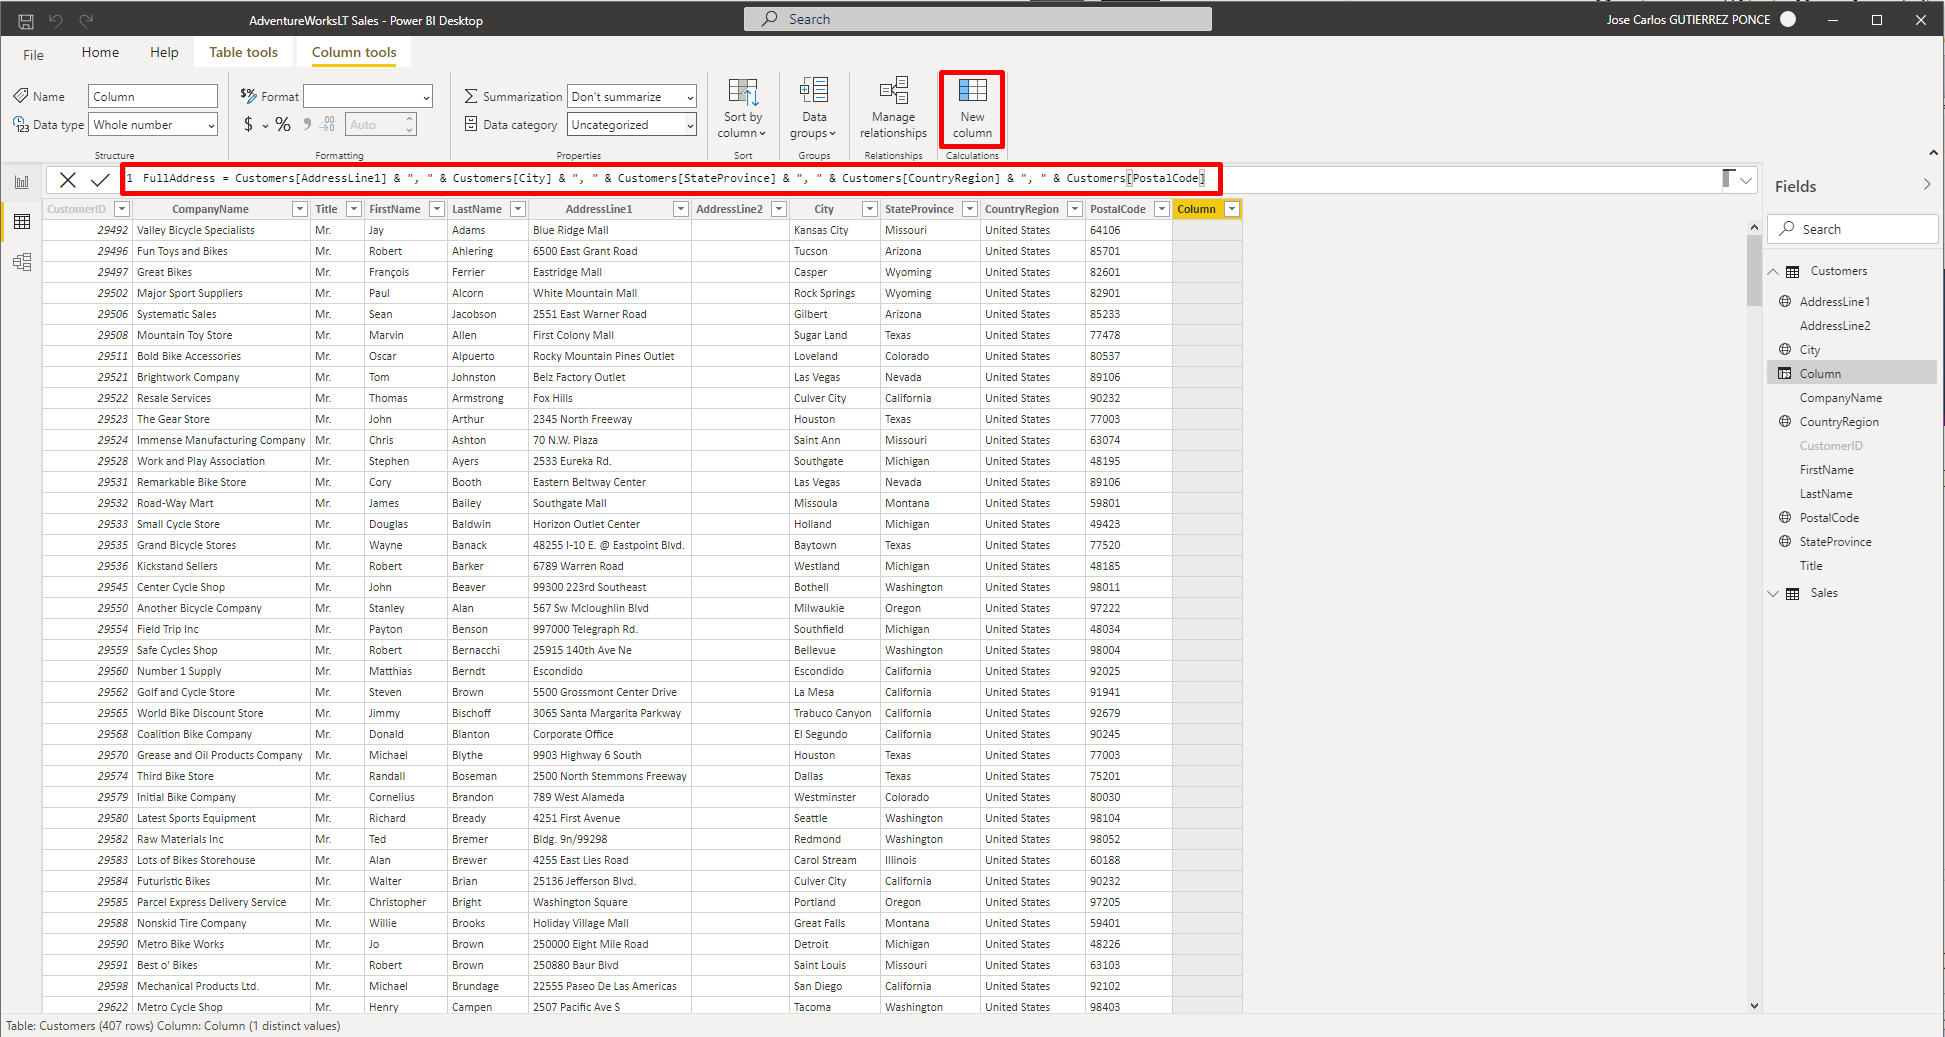
\includegraphics[width=14cm]{./images/34} 
	\end{center}
	
\textbf{2.22. En el panel \textbf{Fields} \textbf{(Fields)}, haga clic en \textbf{Sales}.}

    \begin{center}
		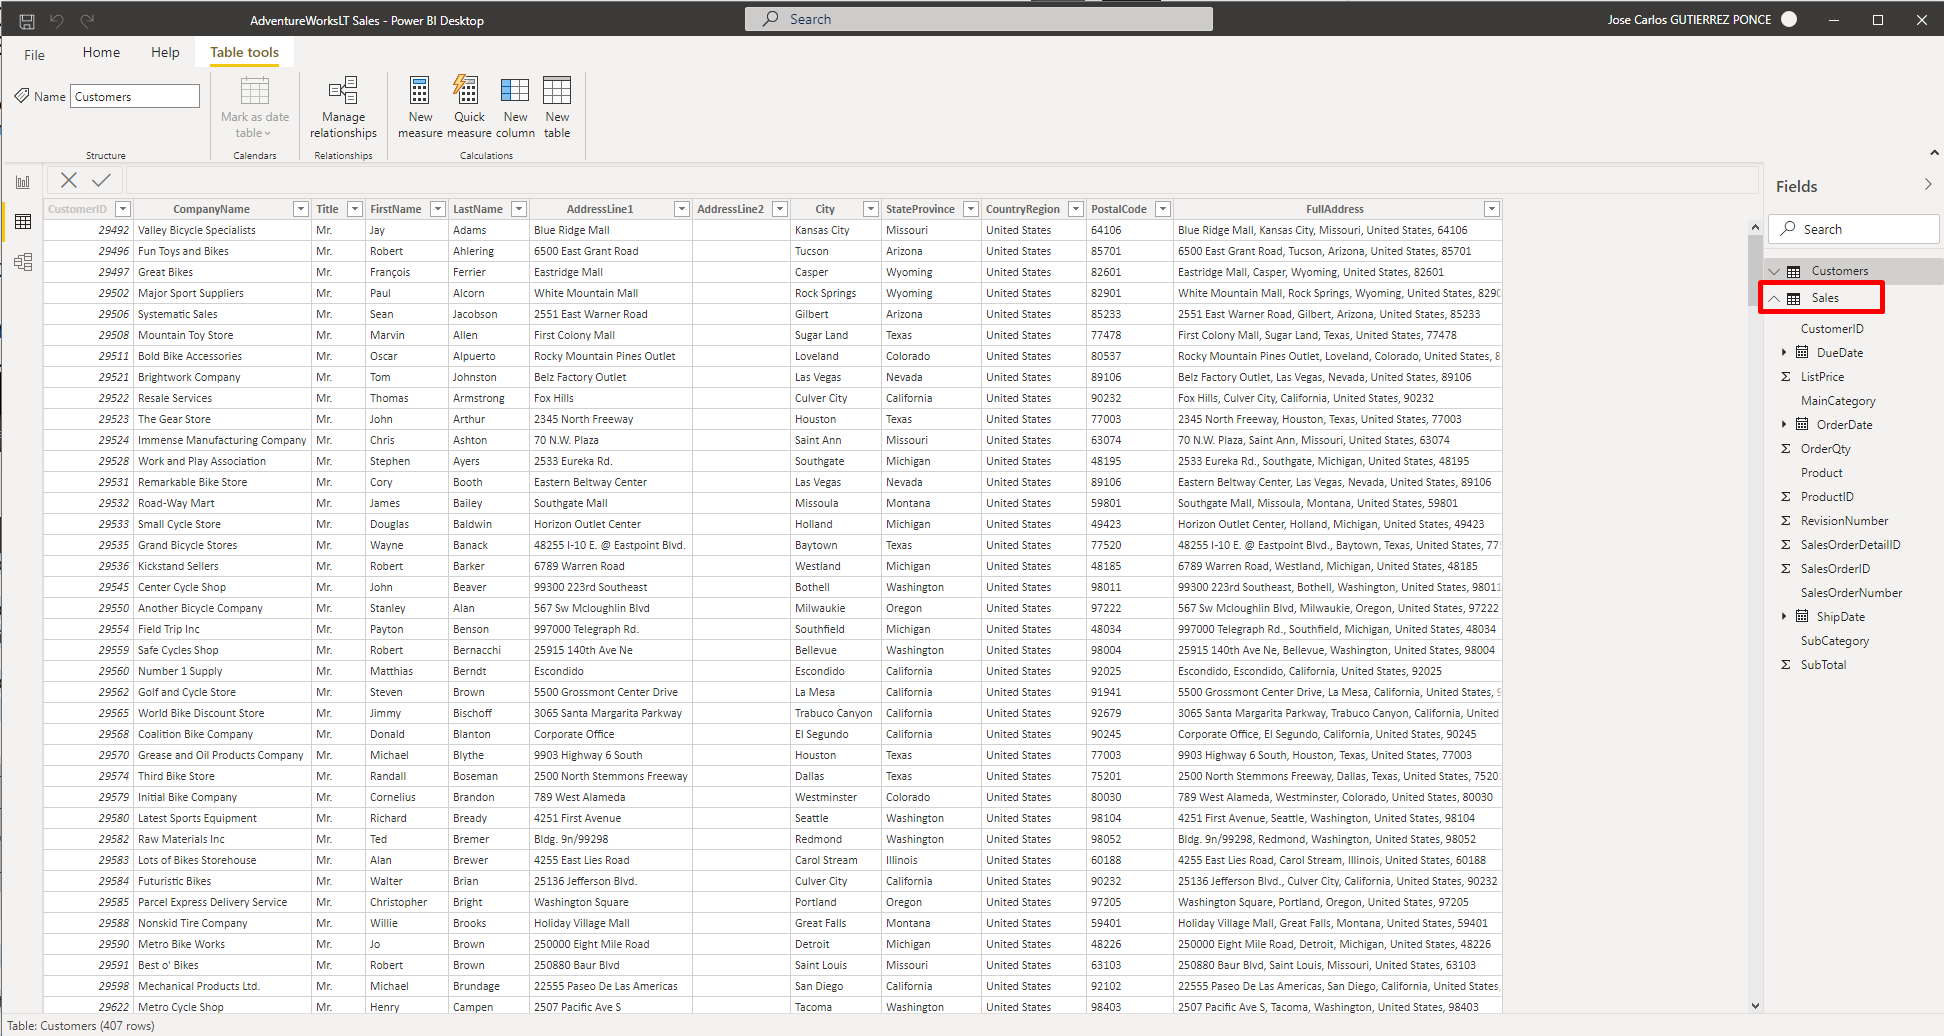
\includegraphics[width=14cm]{images/35.png} 
	\end{center}
\newpage	
\textbf{2.23. Haga clic con el botón derecho en la columna \textbf{RevisionNumber} y haga clic en \textbf{Delete}.}

    \begin{center}
		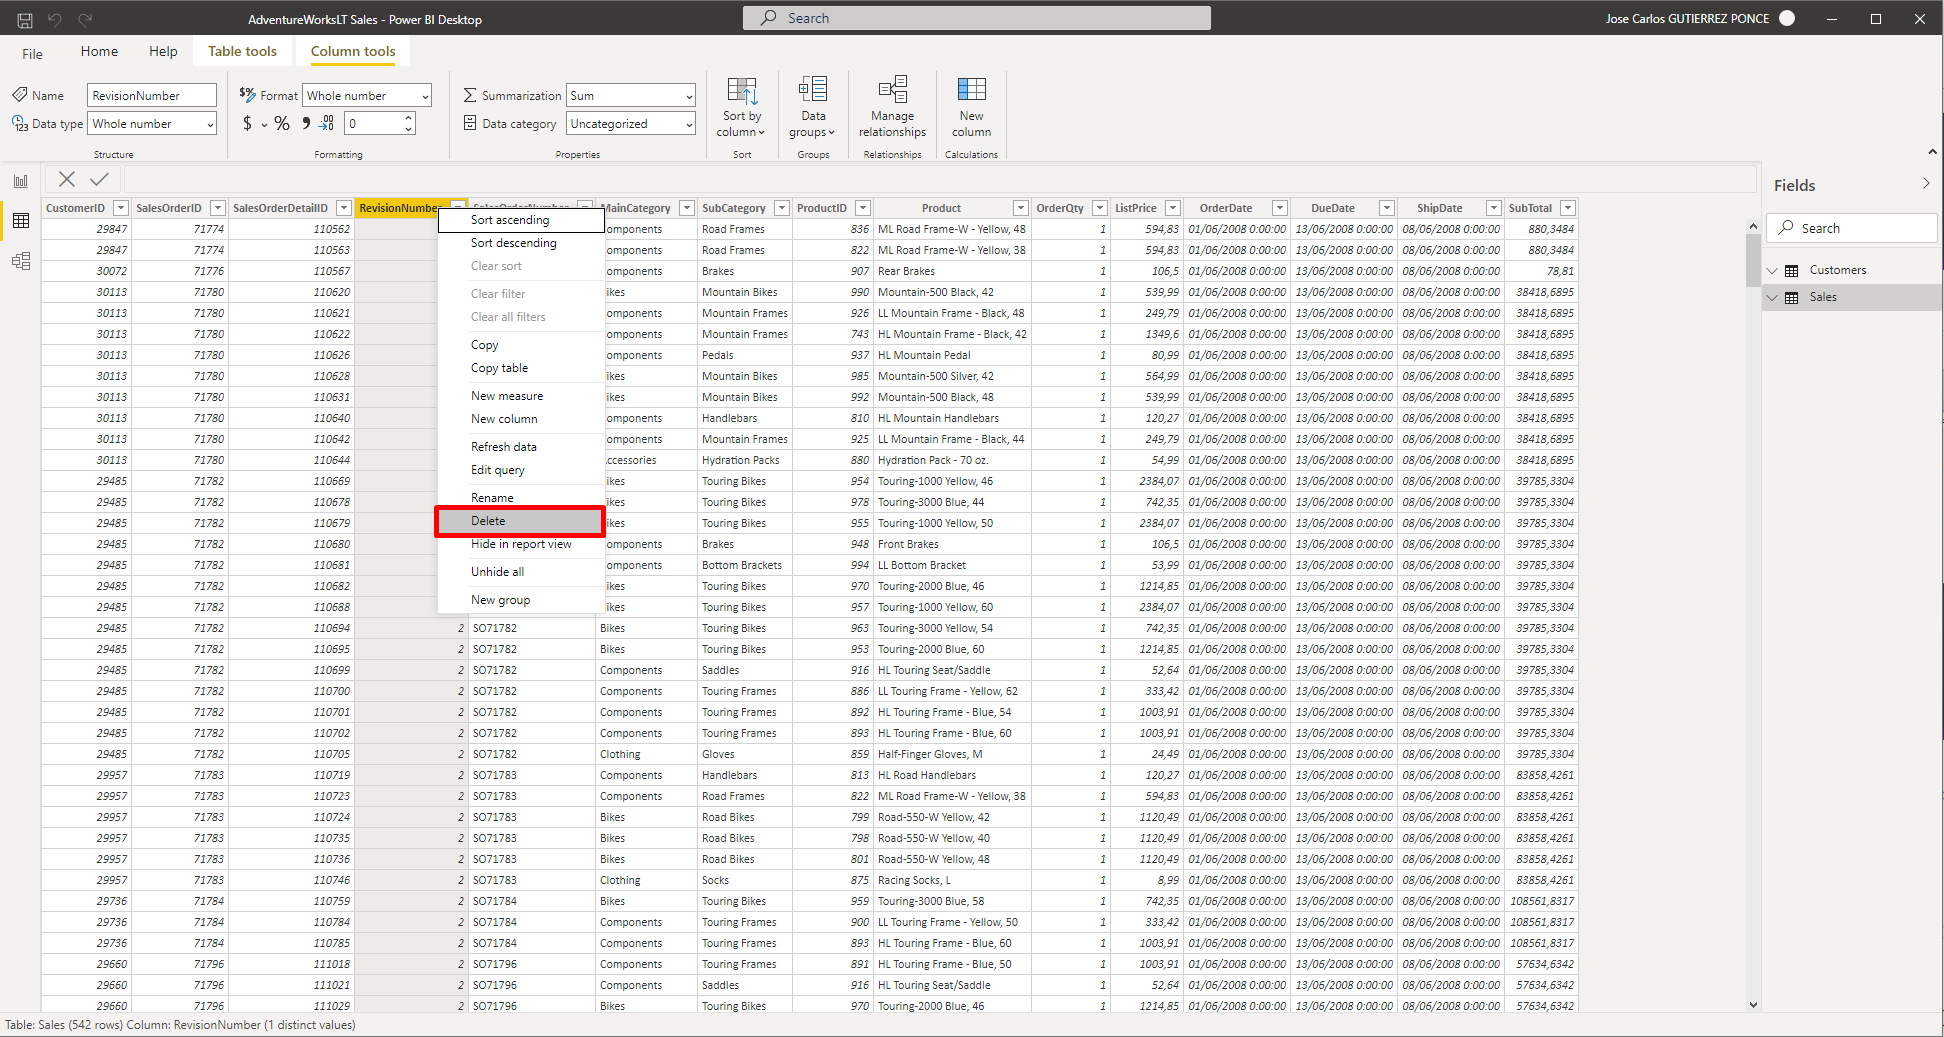
\includegraphics[width=14cm]{./images/36} 
	\end{center}
	
\textbf{2.24. En el cuadro de diálogo \textbf{Delete Column}, haga clic en \textbf{Delete}.}

    \begin{center}
		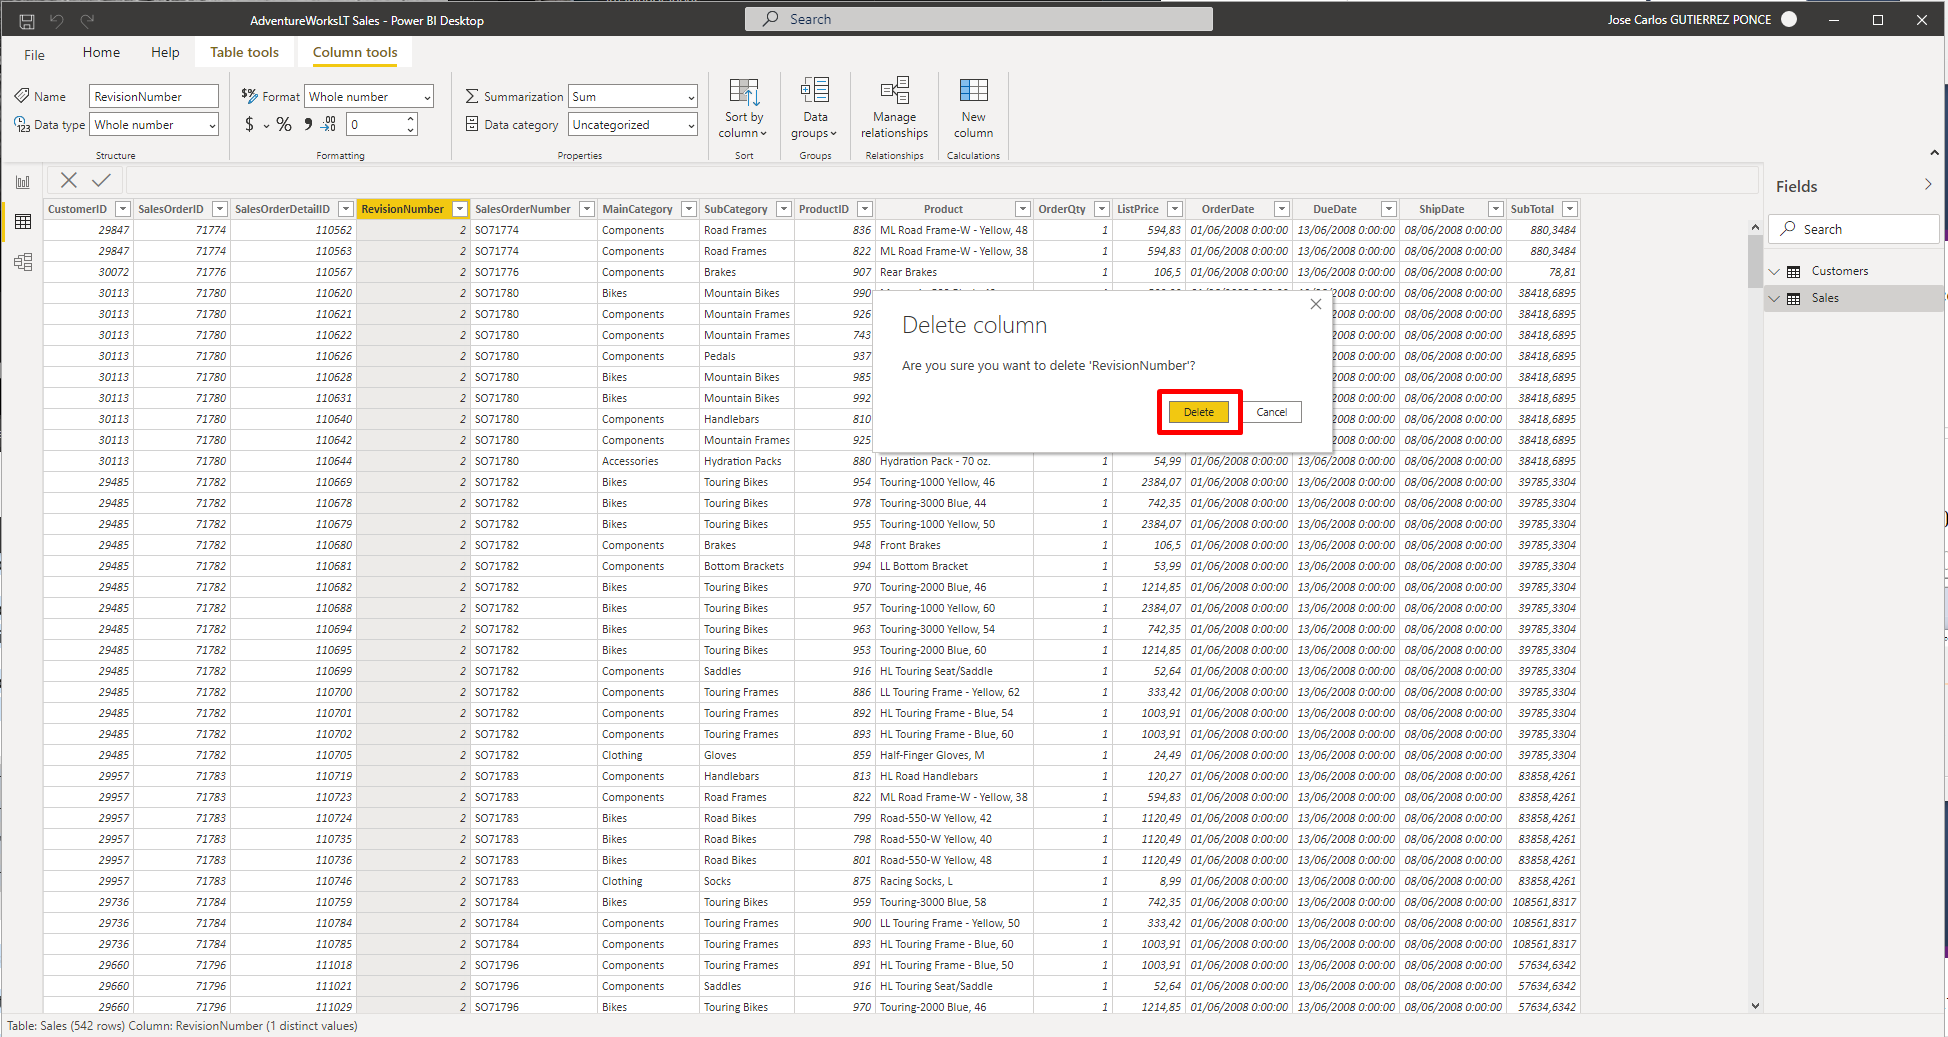
\includegraphics[width=14cm]{./images/37} 
	\end{center}
\newpage	
\textbf{2.25. Haga clic con el botón derecho en la columna \textbf{SalesOrderNumber} y haga clic en \textbf{Delete}.}

    \begin{center}
		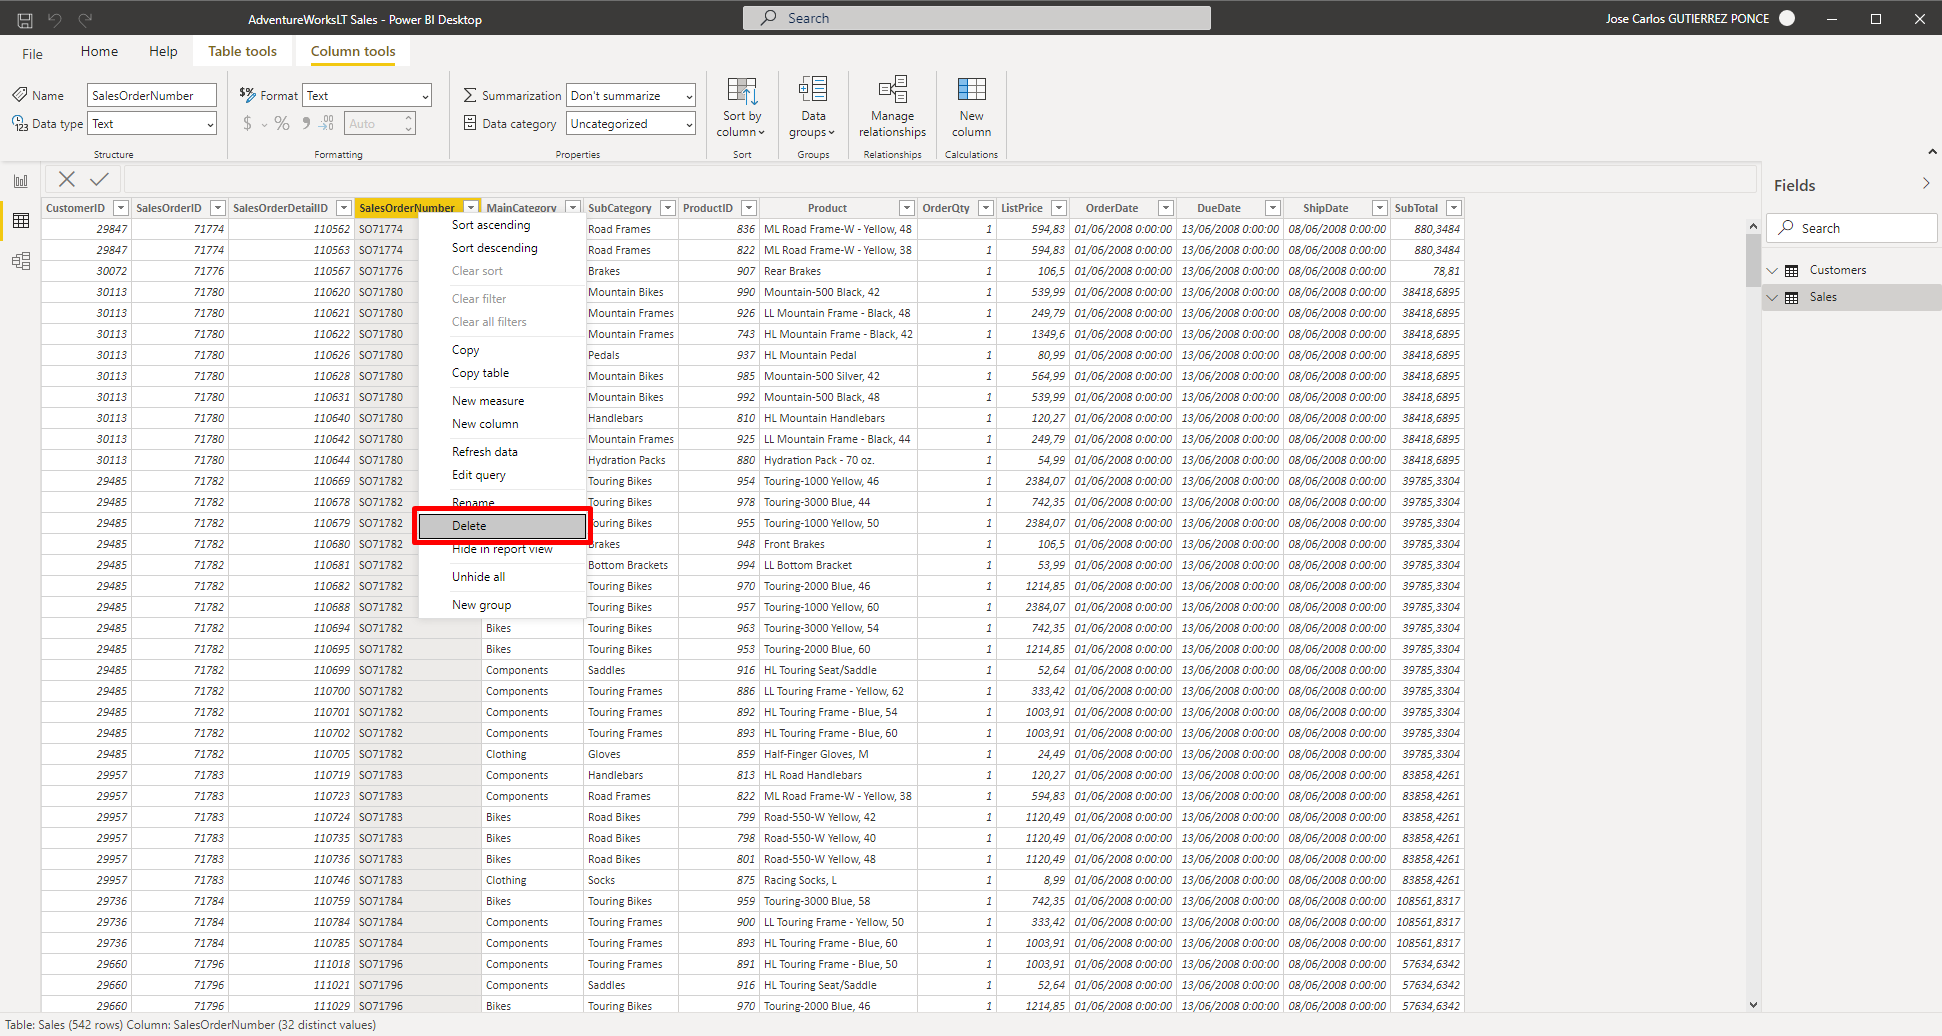
\includegraphics[width=14cm]{./images/38} 
	\end{center}
	
\textbf{2.26. En el cuadro de diálogo \textbf{Delete Column}, haga clic en \textbf{Delete}.}

    \begin{center}
		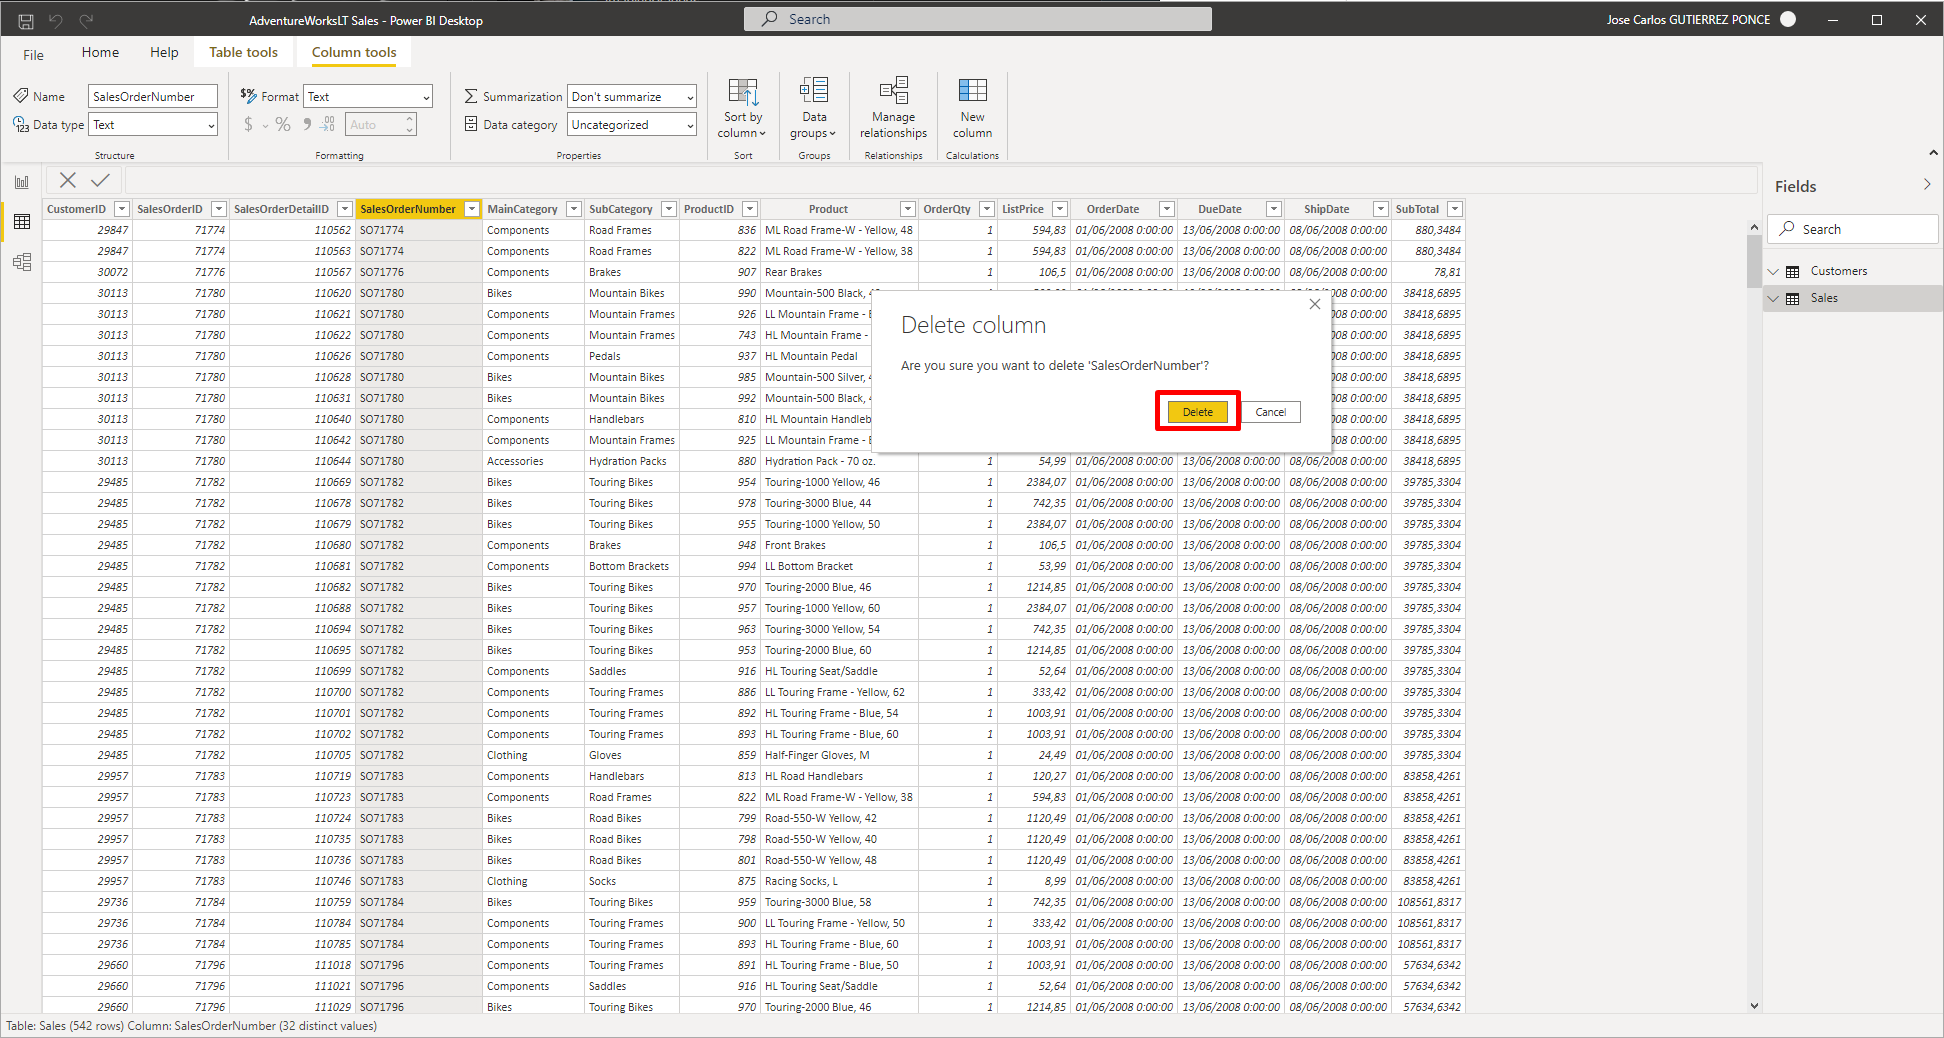
\includegraphics[width=14cm]{./images/39} 
	\end{center}
\newpage	
\textbf{2.28. Haga clic con el botón derecho en la columna \textbf{CustomerID} y luego haga clic en \textbf{Hide in ReportView}.}

    \begin{center}
		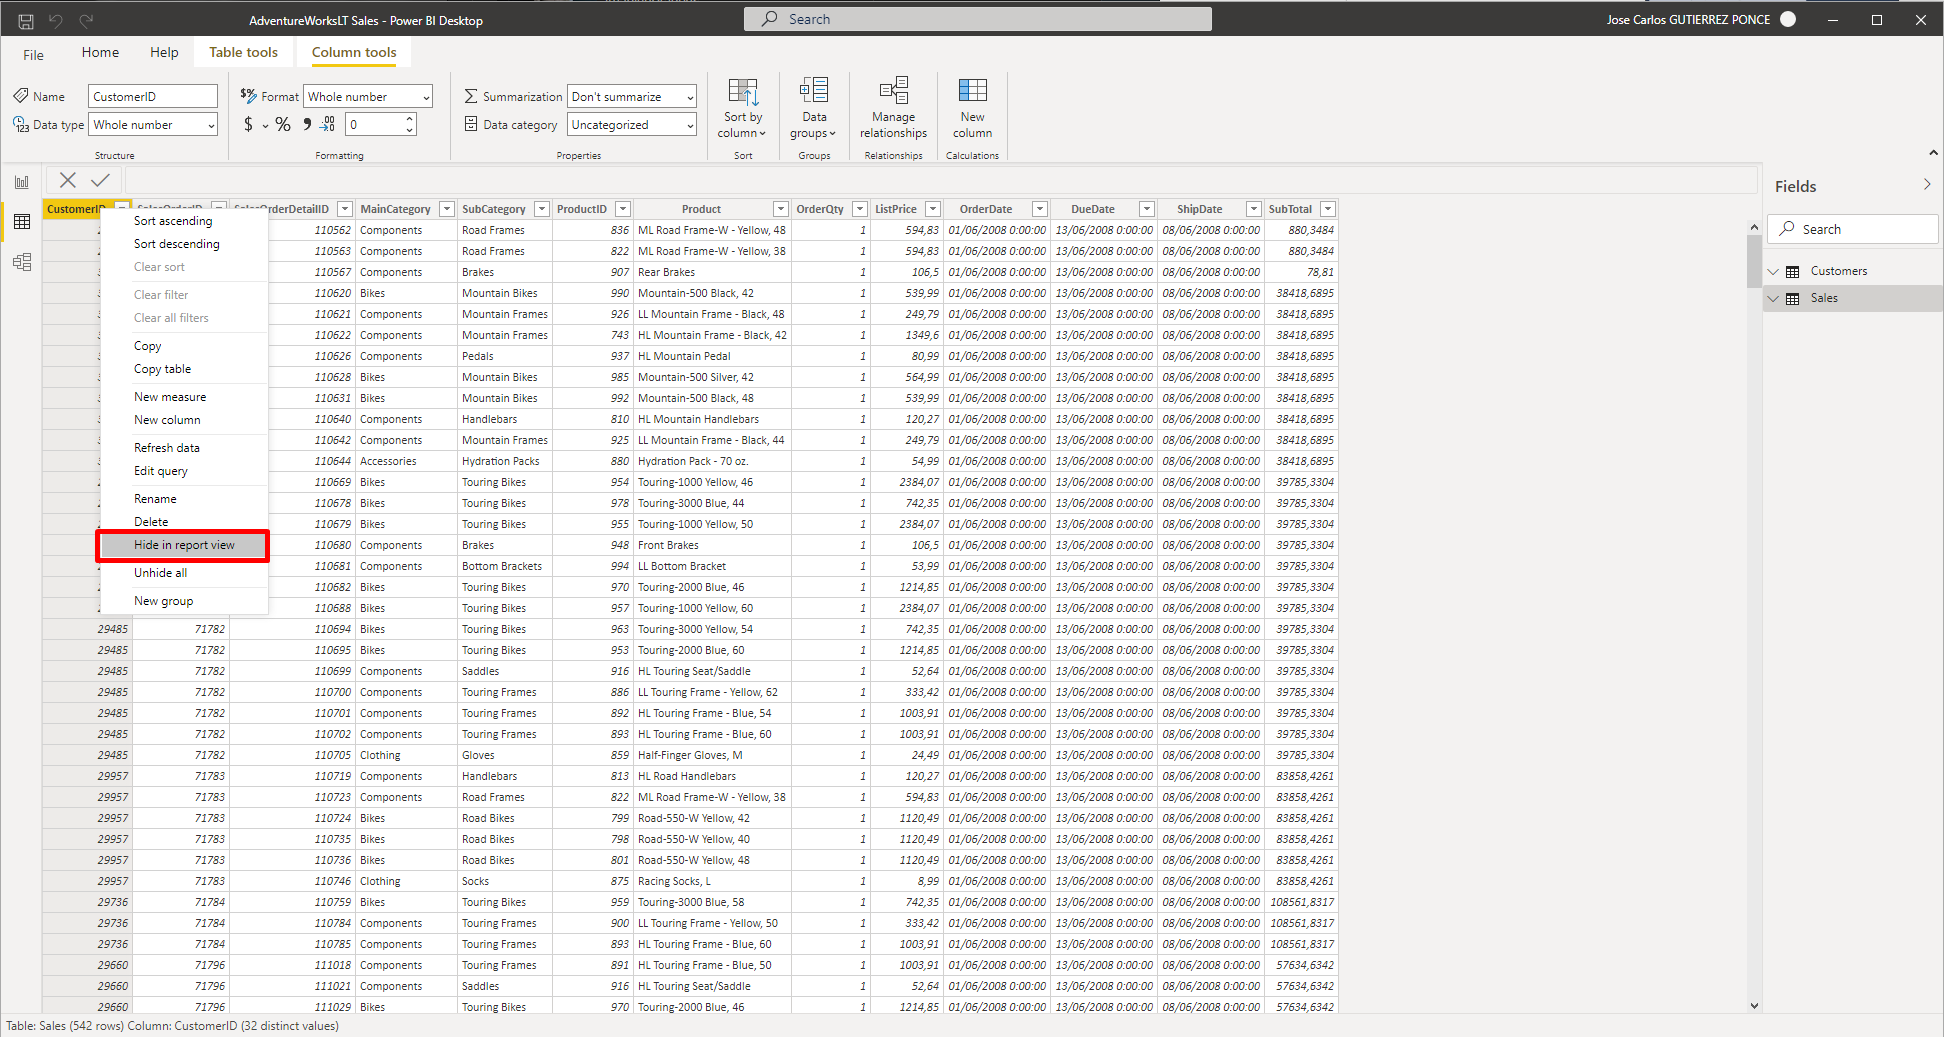
\includegraphics[width=14cm]{./images/40} 
	\end{center}
	
\textbf{2.29. Haga clic con el botón derecho en la columna \textbf{SalesOrderID} y luego haga clic en \textbf{Hide in ReportView}.}

    \begin{center}
		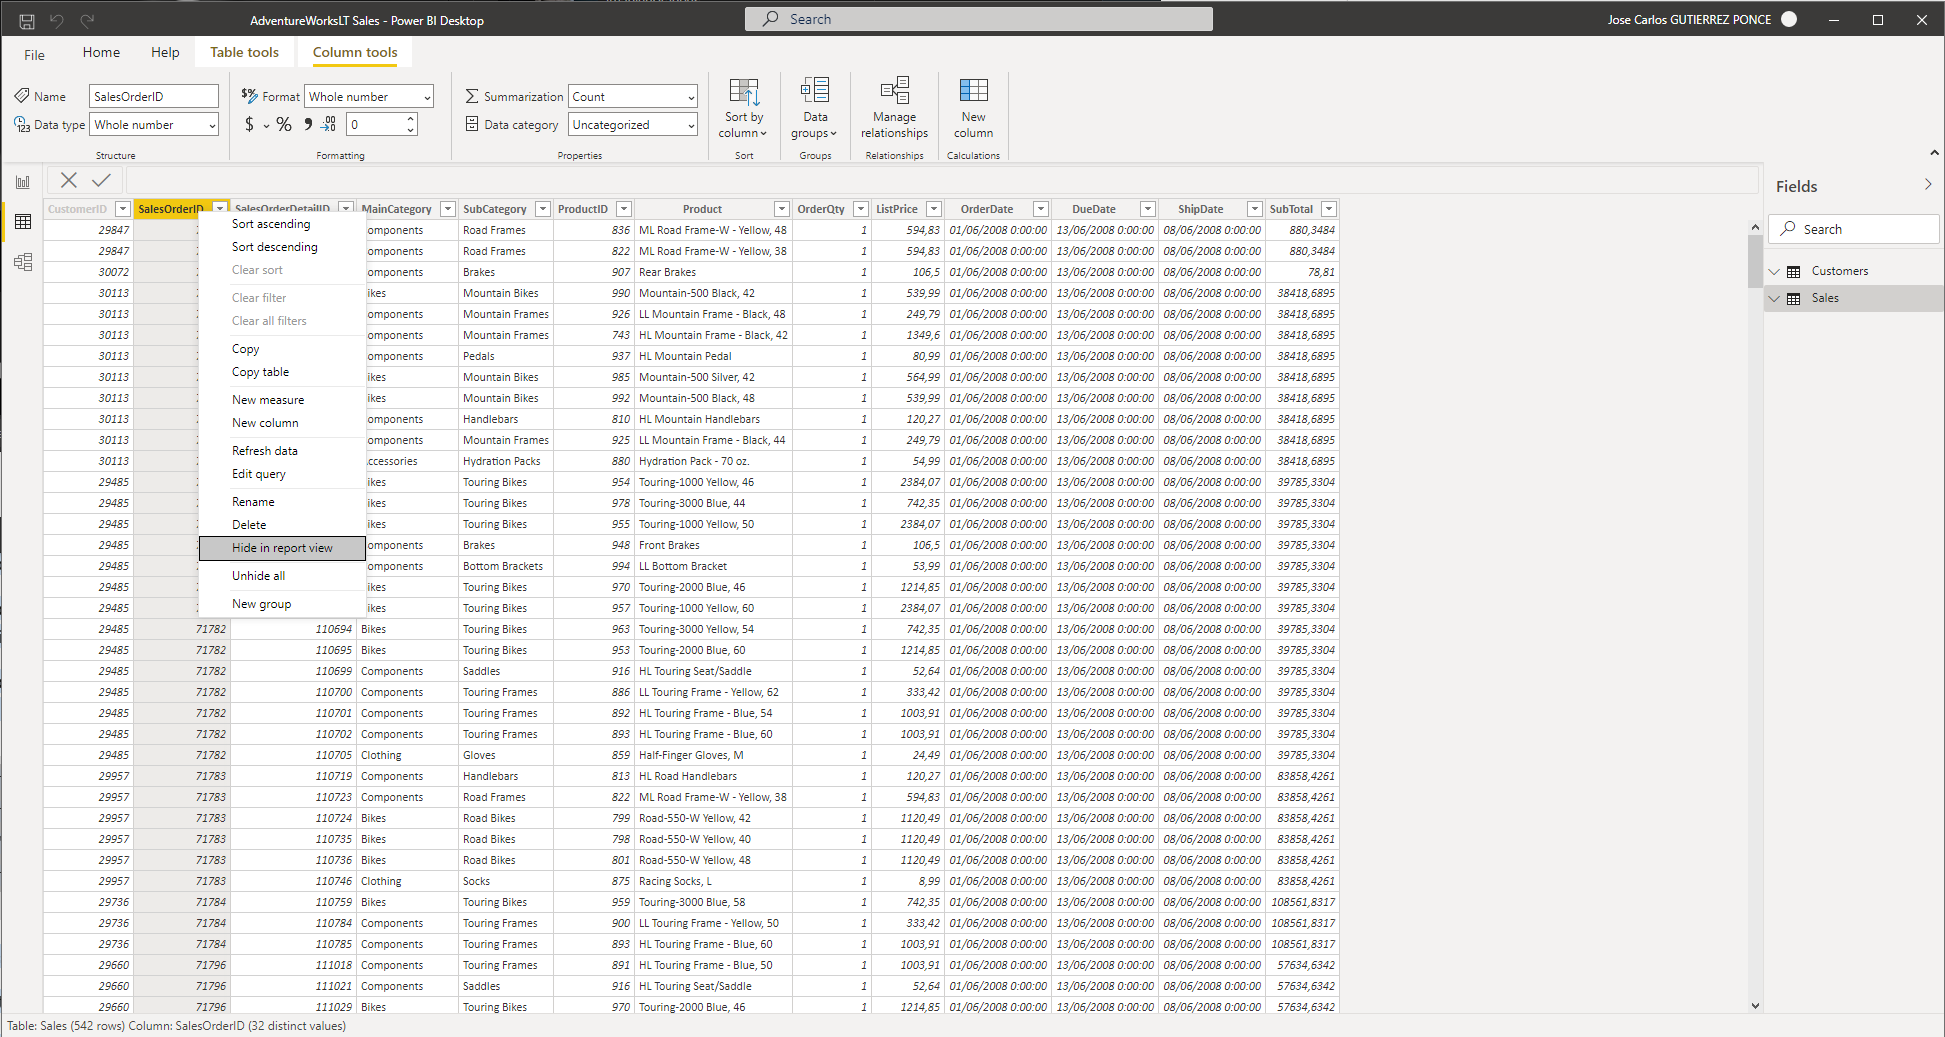
\includegraphics[width=14cm]{./images/41} 
	\end{center}
\newpage	
\textbf{2.30. Haga clic con el botón derecho en la columna \textbf{SalesOrderDetailID} y luego haga clic en \textbf{Hide in ReportView}.}

    \begin{center}
		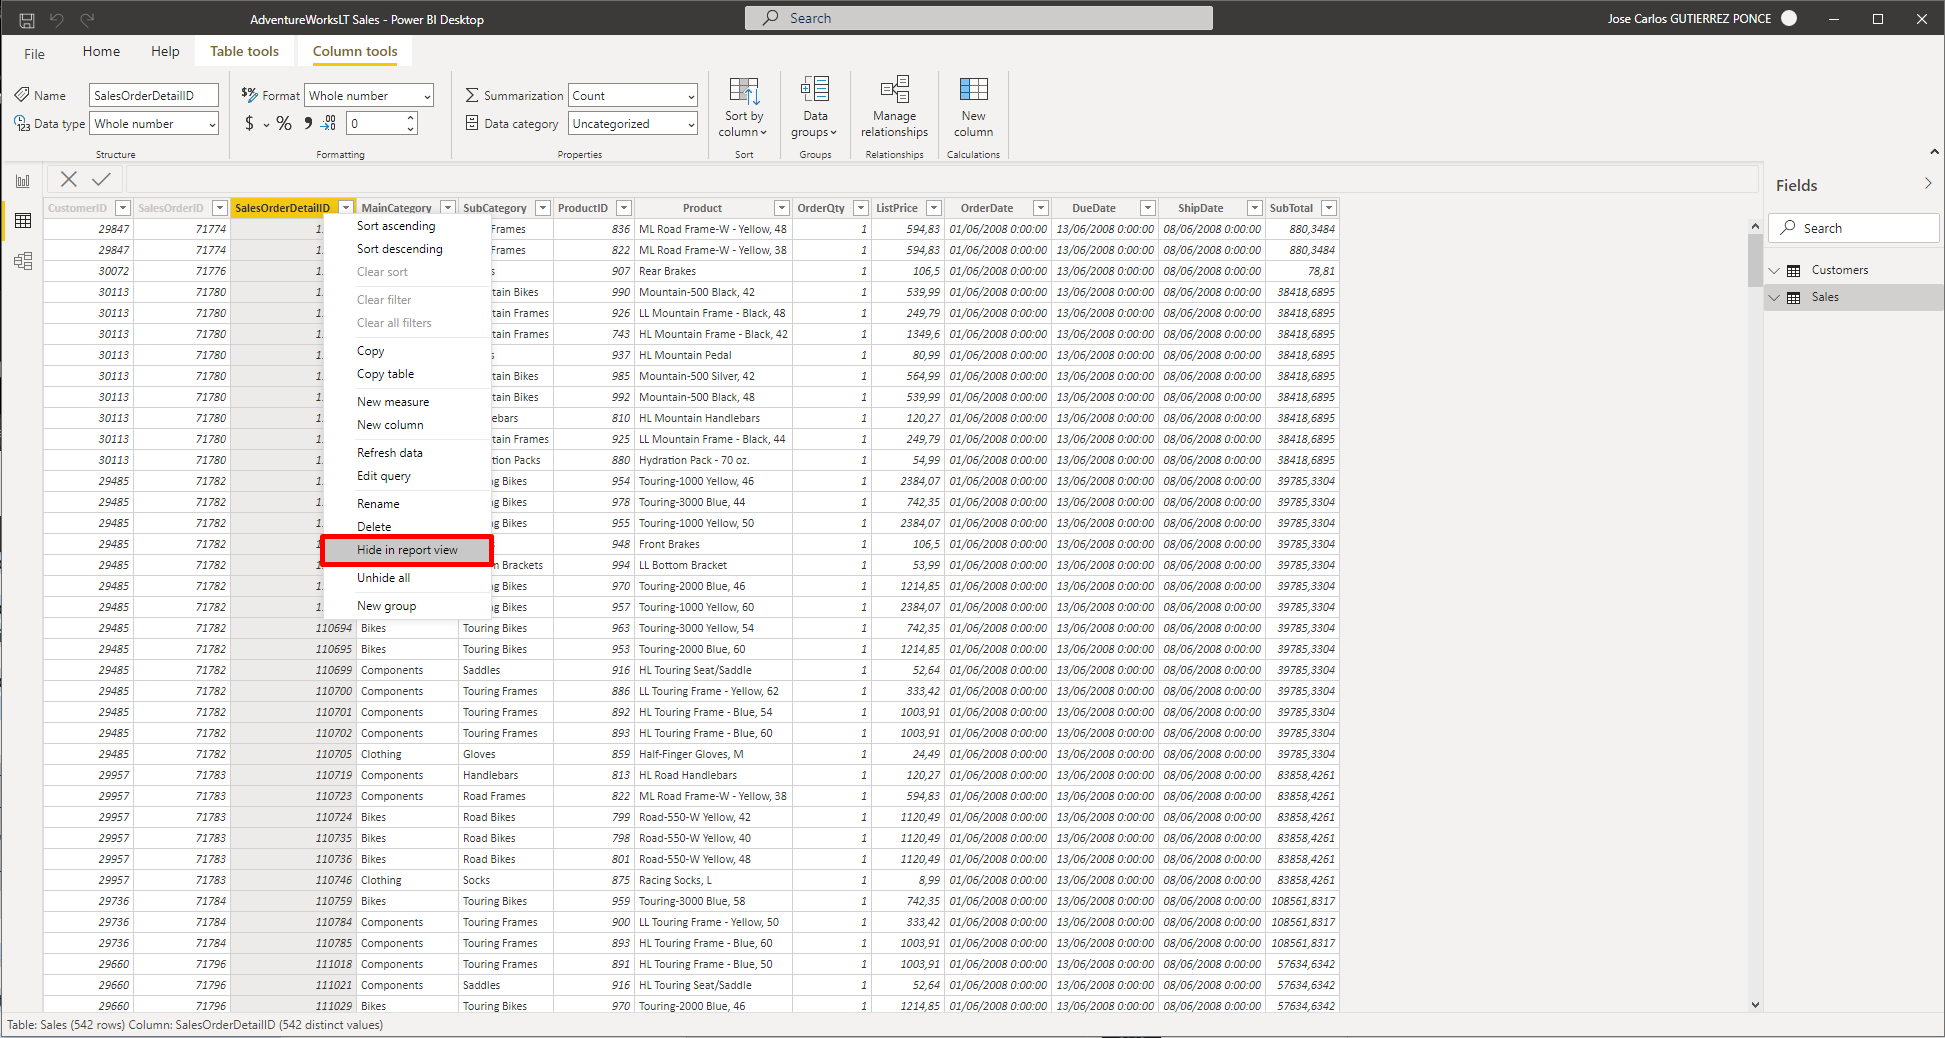
\includegraphics[width=14cm]{./images/42} 
	\end{center}
	
\textbf{2.31. En la cinta \textbf{Modeling}, en el grupo \textbf{Calculations}, haga clic en \textbf{NewColumn} y luego en la barra de fórmulas, escriba la siguiente expresión y presione Enter:}

    \begin{center}
		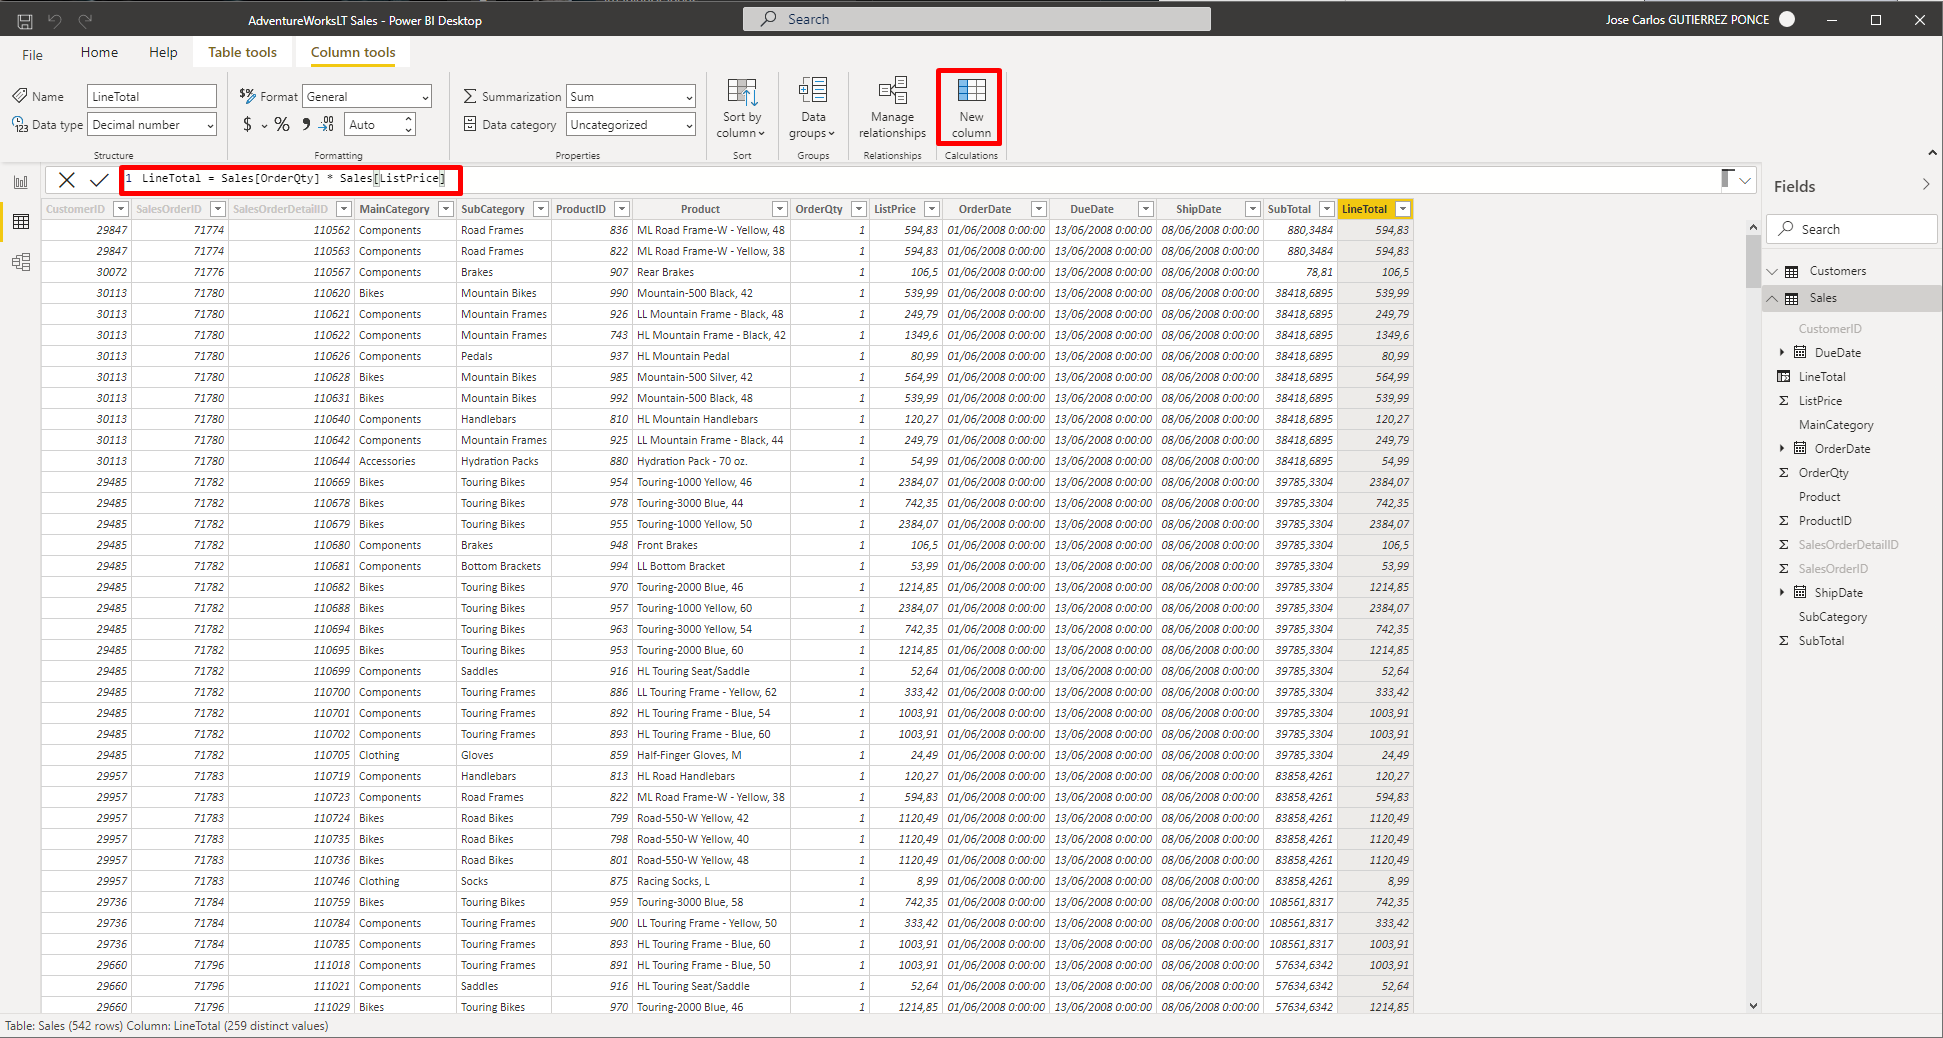
\includegraphics[width=14cm]{./images/43} 
	\end{center}
\newpage	
\textbf{2.32. Haga clic en el encabezado de la columna \textbf{LineTotal}.}

    \begin{center}
		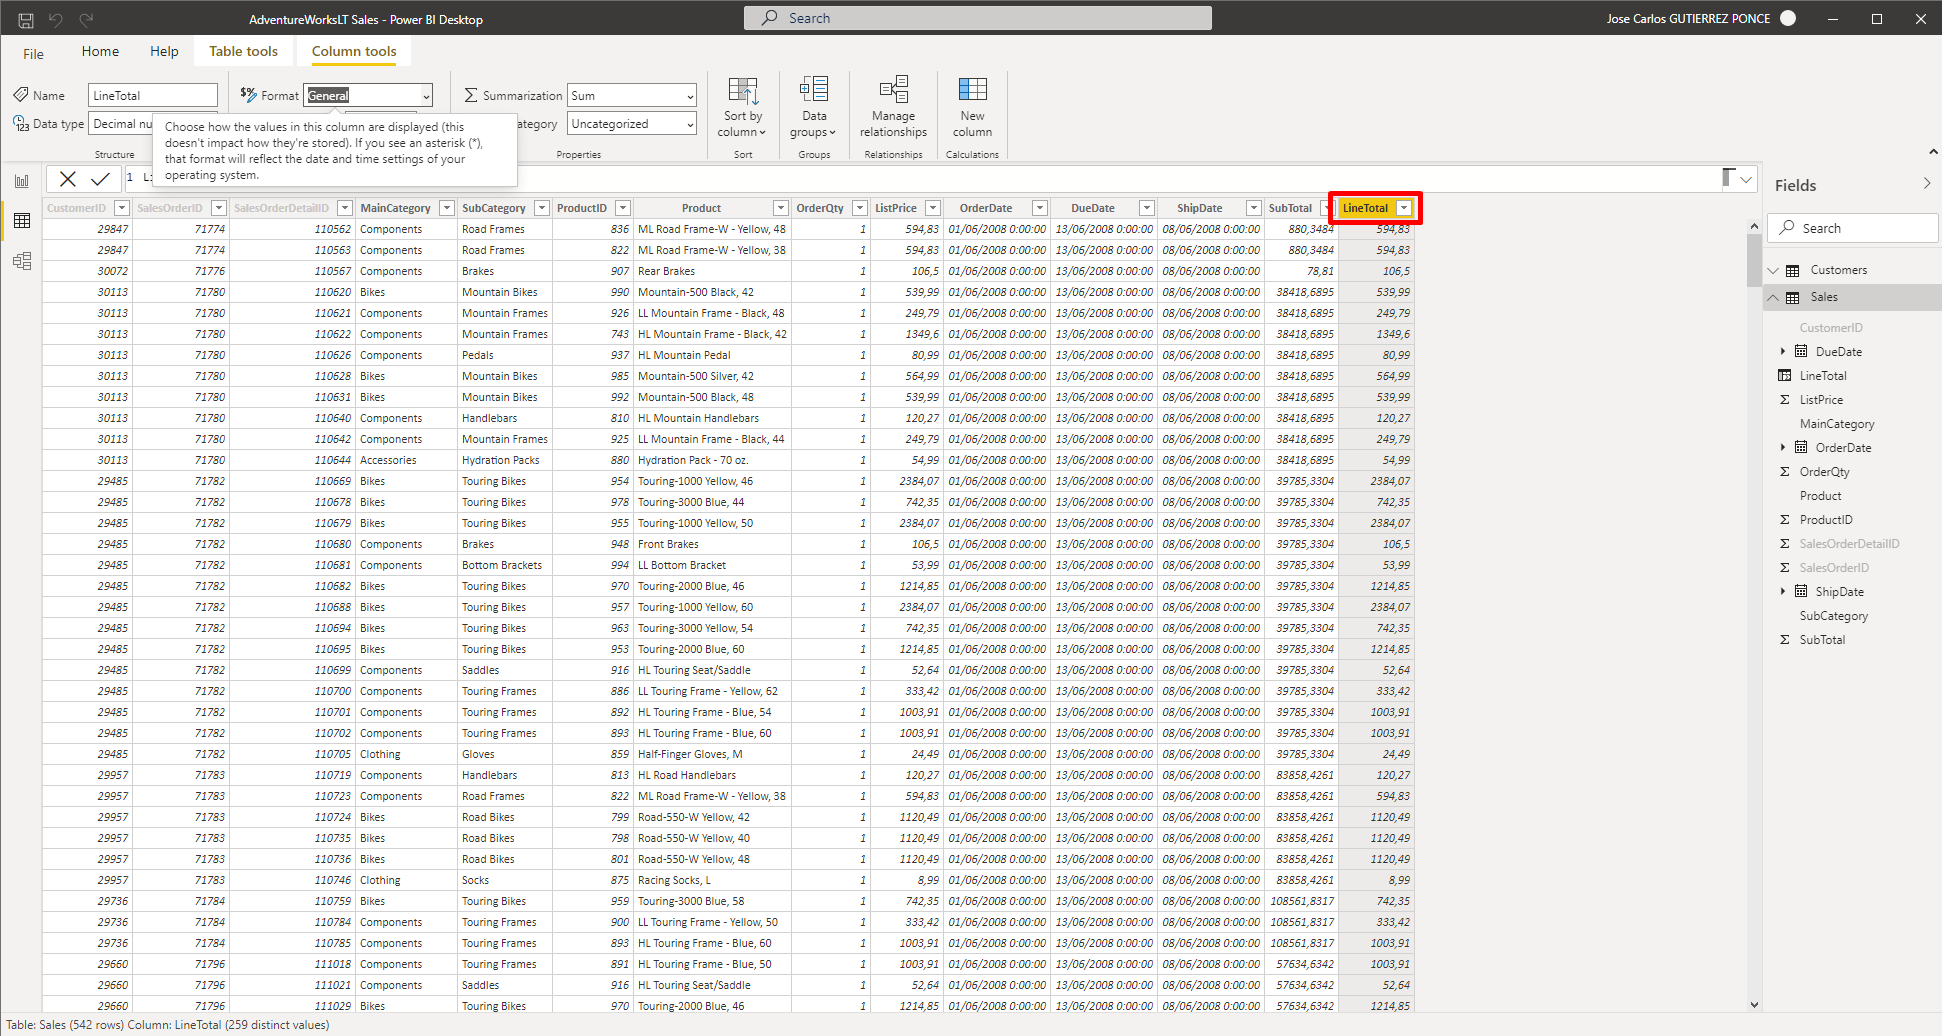
\includegraphics[width=14cm]{./images/44} 
	\end{center}
	
\textbf{2.33. En la cinta \textbf{Modeling}, en el grupo \textbf{Formatting}, haga clic en \textbf{Format:General}, señale \textbf{Currency} y luego haga clic en \textbf{\$ English (United States)}.}

    \begin{center}
		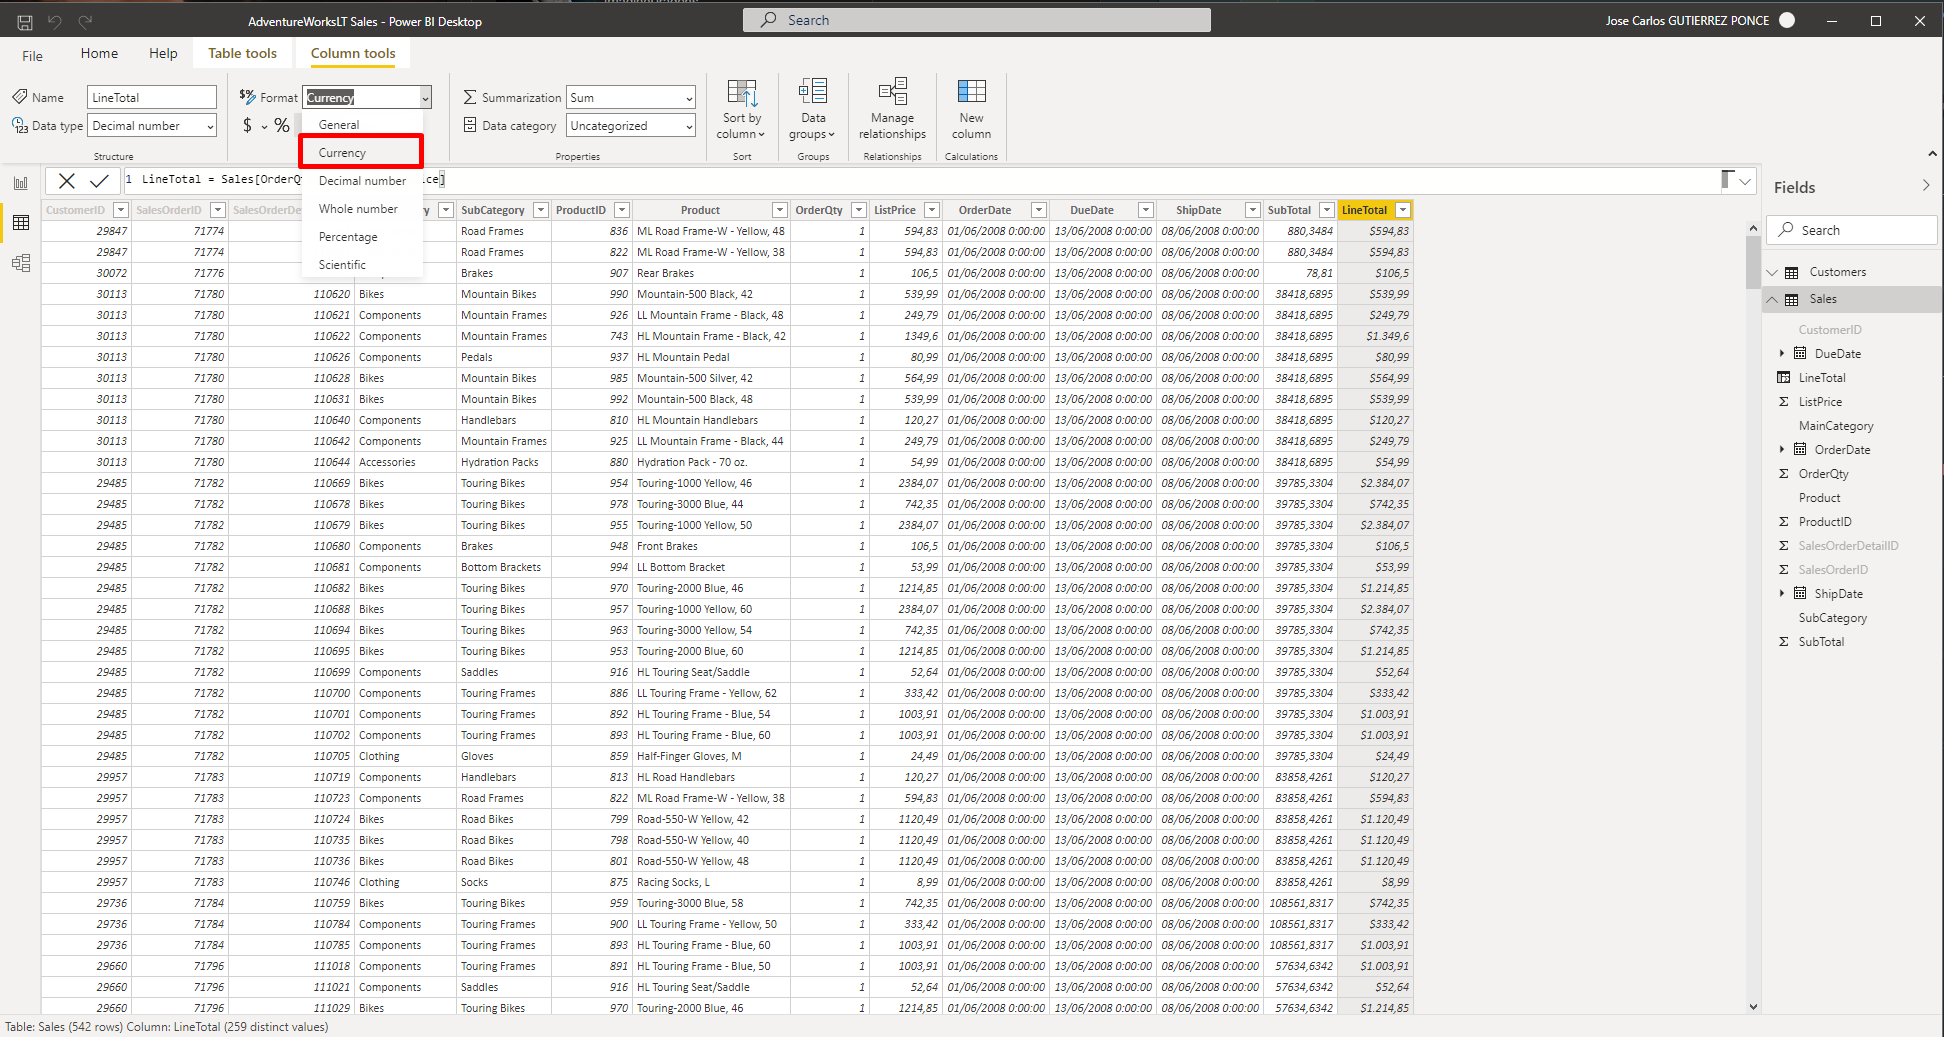
\includegraphics[width=14cm]{./images/45} 
	\end{center}
\newpage	
\textbf{2.34. En la cinta \textbf{Modeling}, en el grupo \textbf{Calculations}, haga clic en \textbf{NewMeasure} y luego en la barra de fórmulas, escriba la siguiente expresión y presione Enter.}

    \begin{center}
		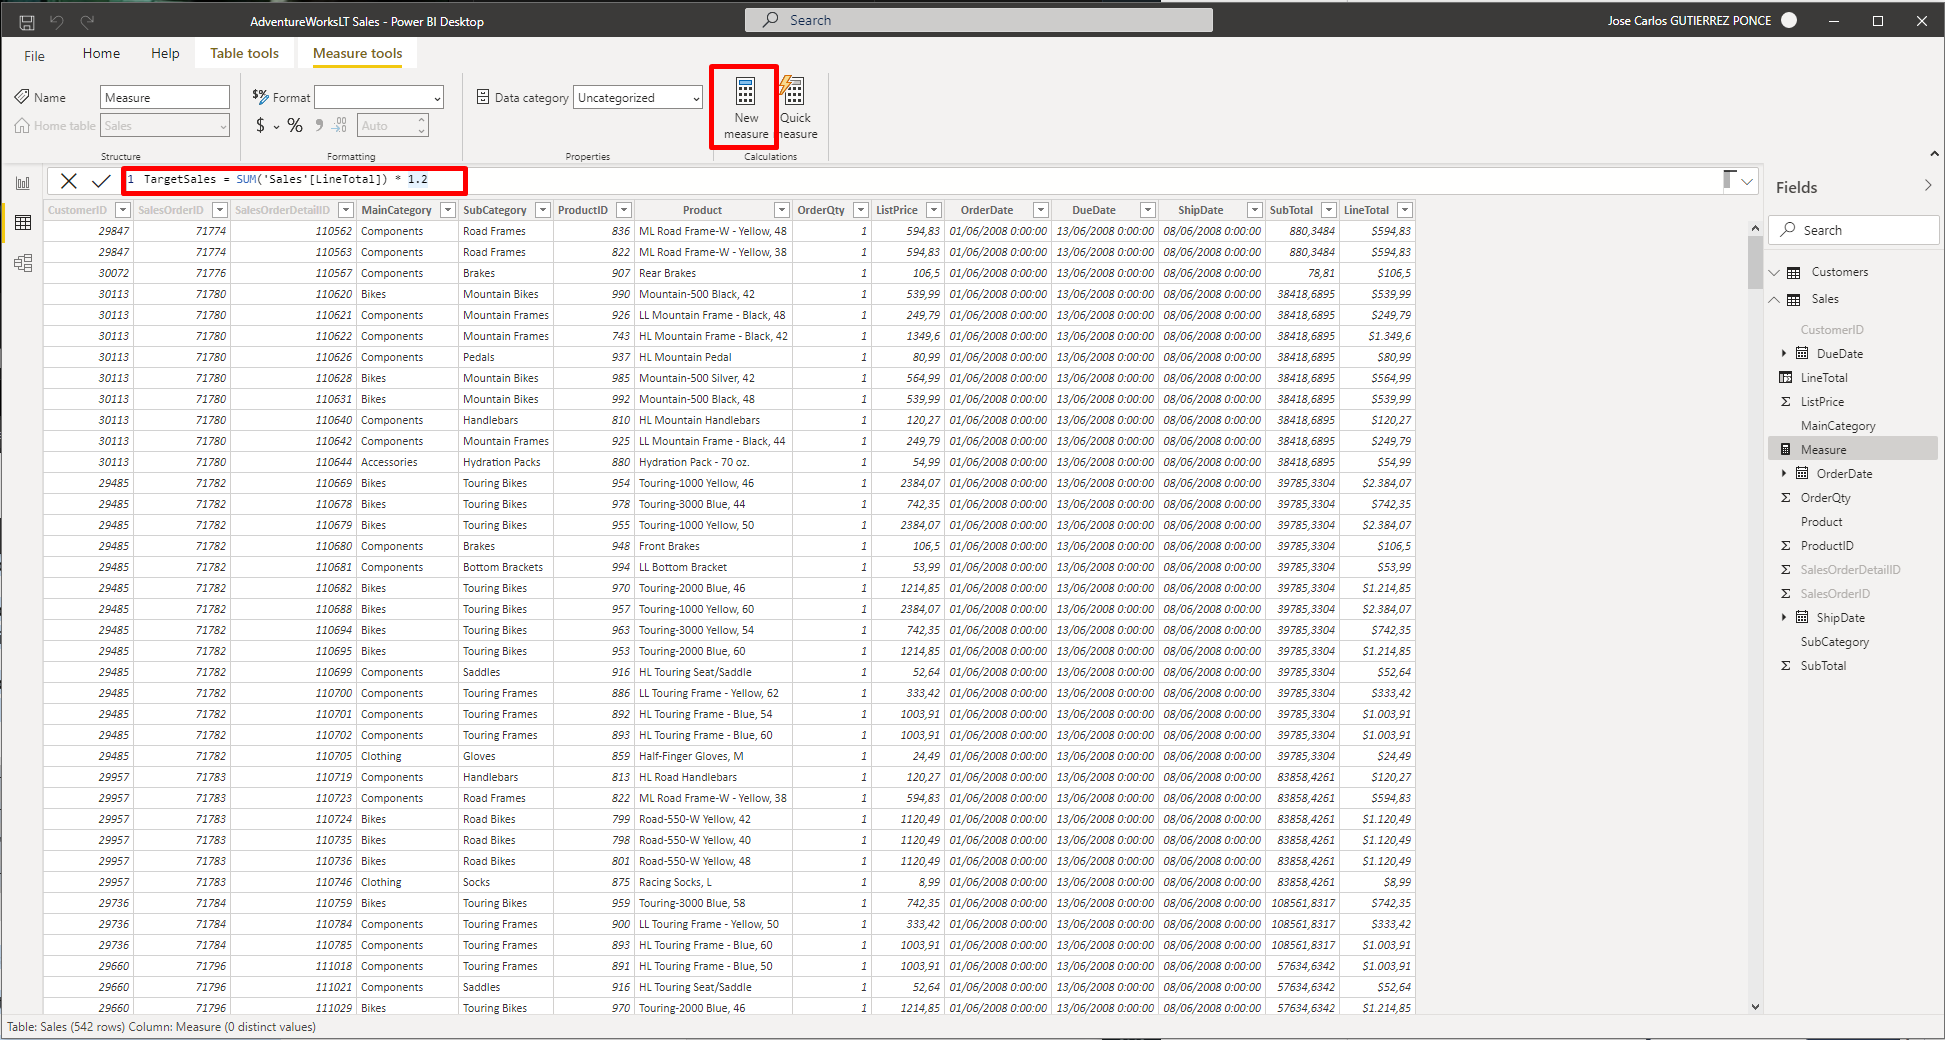
\includegraphics[width=14cm]{./images/46} 
	\end{center}
	
\textbf{2.35. Haga clic en \textbf{Save} y deje Power BI Desktop abierto para la siguiente tarea.}

    \begin{center}
		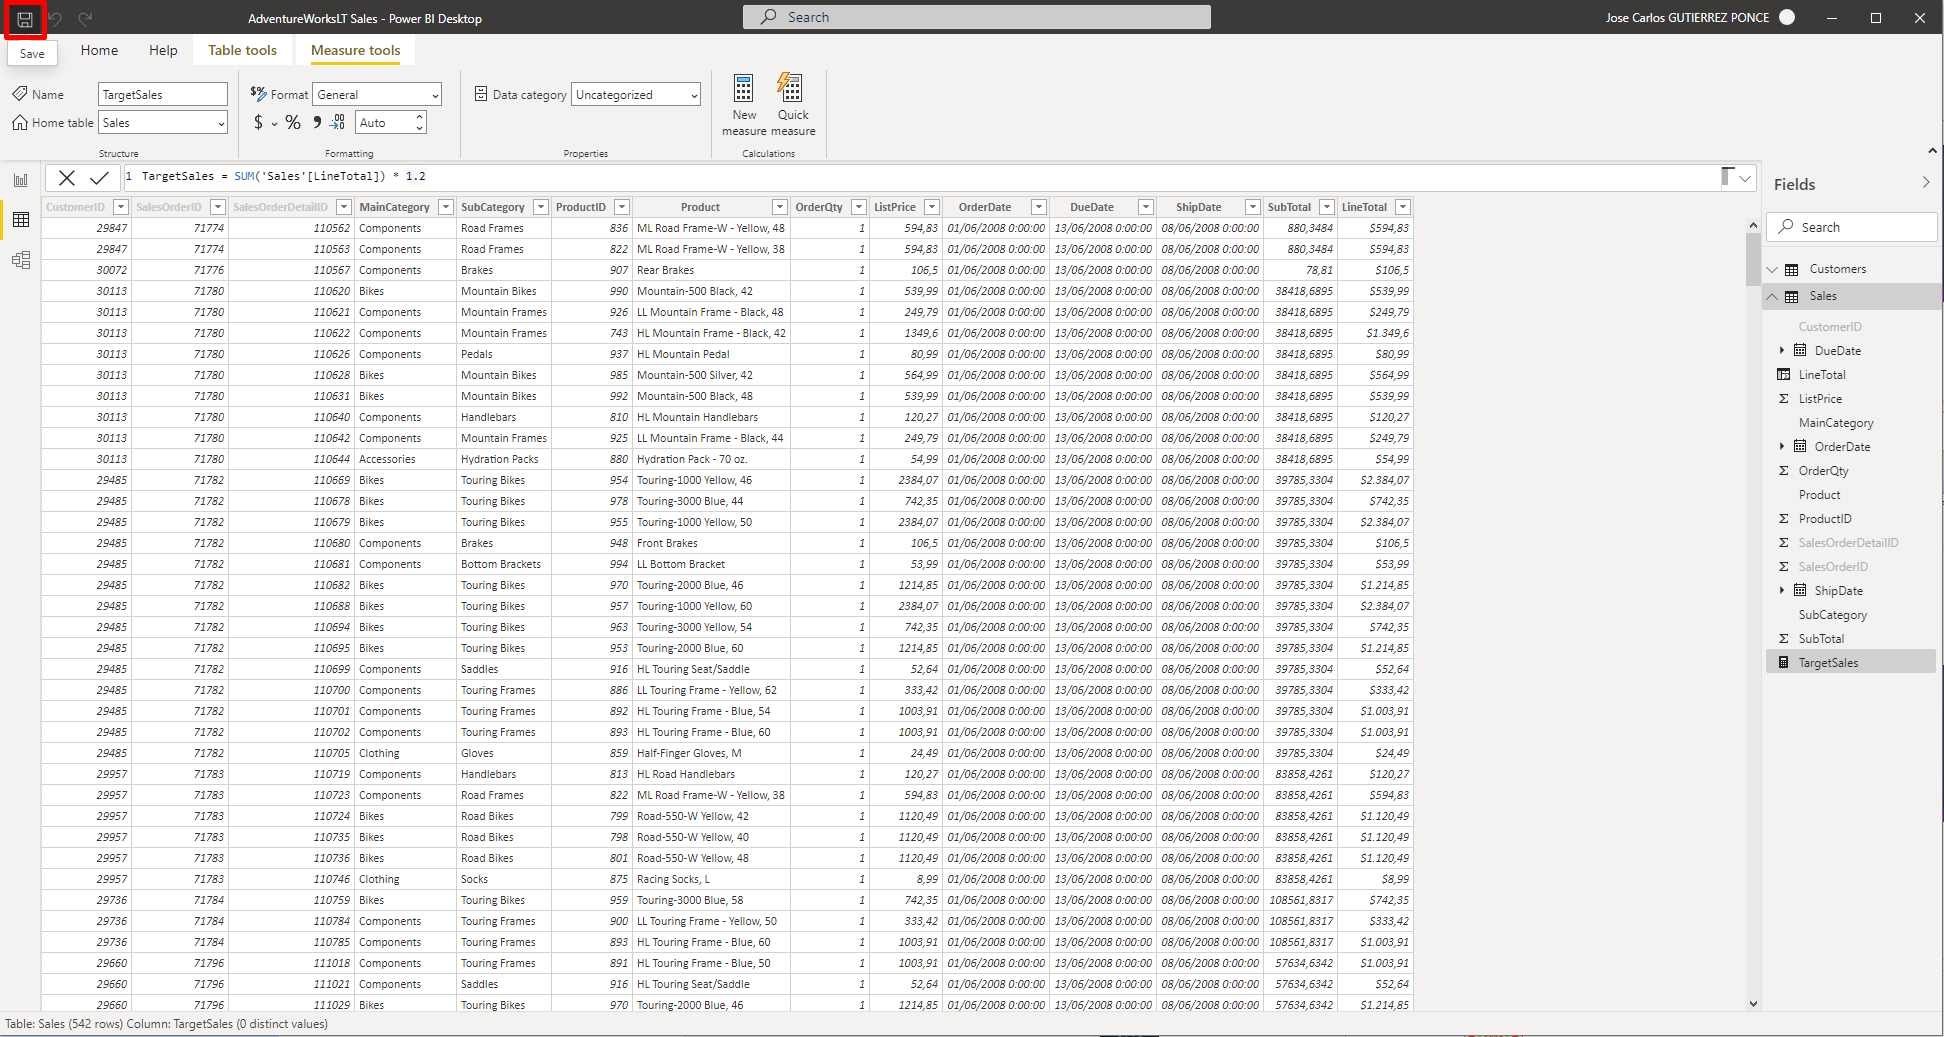
\includegraphics[width=14cm]{./images/47} 
	\end{center}

	
	
	
\newpage
\section{Combinar Data}

\textbf{3.1. En el \textbf{Explorador de archivos} y luego abra el archivo \textbf{States.xlsx}.}

    \begin{center}
		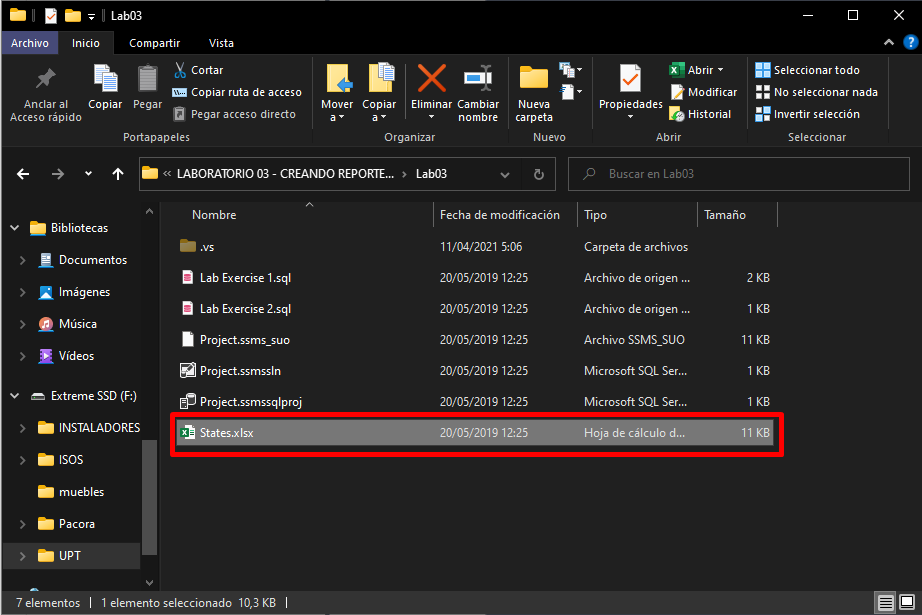
\includegraphics[width=14cm]{./images/48} 
	\end{center}
\newpage
\textbf{3.2. En la hoja de trabajo de \textbf{States}, seleccione todos los valores en las dos columnas y luego presione Ctrl + C.}

    \begin{center}
		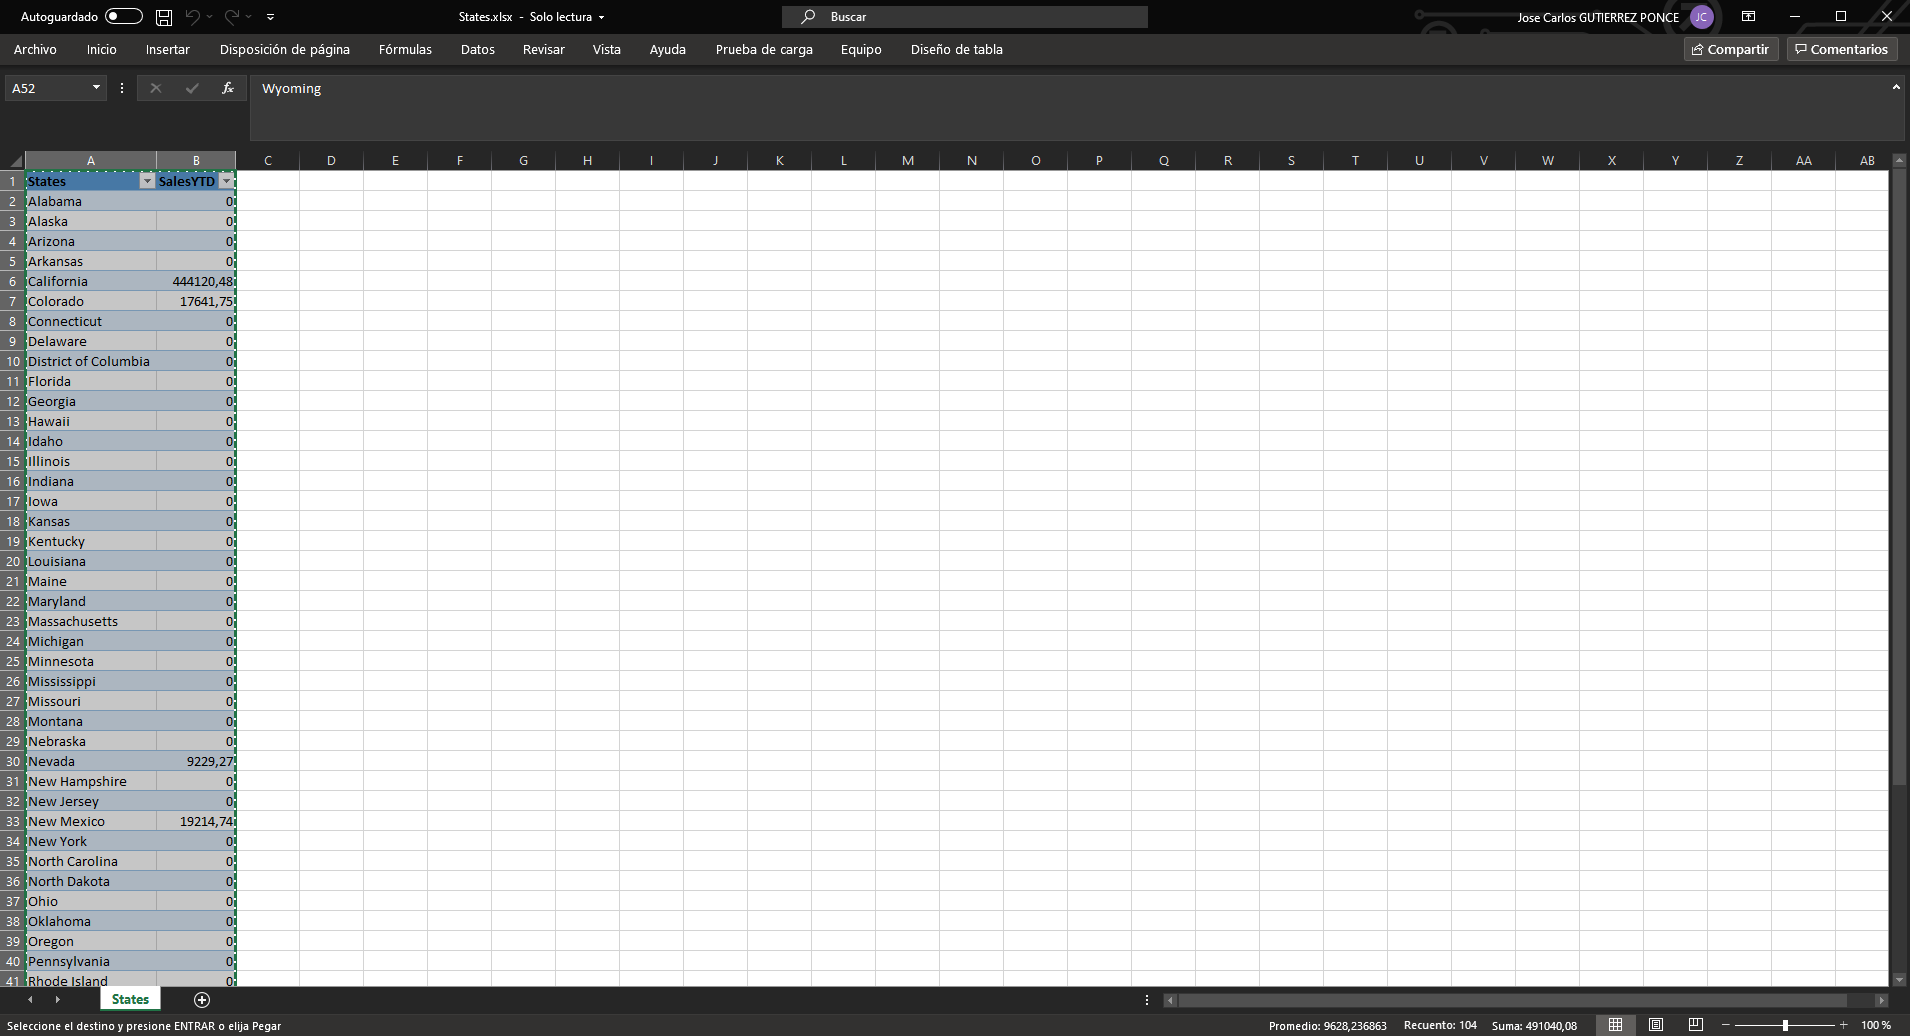
\includegraphics[width=14cm]{./images/49} 
	\end{center}

\textbf{3.3. En Power BI Desktop, en la cinta \textbf{Home}, haga clic en Enter Data.}

    \begin{center}
		\includegraphics[width=14cm]{./images/50} 
	\end{center}
\newpage
\textbf{3.4. En el cuadro de diálogo Crear tabla, haga clic en la tabla y luego presione Ctrl + V. Power BI detecta que la primera fila es un encabezado de columna.}

    \begin{center}
		\includegraphics[width=14cm]{./images/51} 
	\end{center}

\textbf{3.5. En el cuadro \textbf{Name}, escriba \textbf{Sales by State} y luego haga clic en \textbf{Load}.}

    \begin{center}
		\includegraphics[width=14cm]{./images/52} 
	\end{center}
\newpage
\textbf{3.6. En la cinta \textbf{Home}, haga clic en \textbf{Get Data} y luego en \textbf{Web}.}

    \begin{center}
		\includegraphics[width=14cm]{./images/53} 
	\end{center}

\textbf{3.7. En el cuadro de diálogo \textbf{From Web}, en el cuadro \textbf{URL}, escriba \url{http://en.wikipedia.org/wiki/List_of_U.S._state_abbreviations} y, a continuación, haga clic en \textbf{OK}.}

    \begin{center}
		\includegraphics[width=14cm]{./images/54} 
	\end{center}
\newpage
\textbf{3.8. En el cuadro de diálogo \textbf{Navigator}, seleccione \textbf{Codes and abbreviations for U.S. states, territories and other regions}. Y luego haga clic en \textbf{Load}.}

    \begin{center}
		\includegraphics[width=14cm]{./images/55} 
	\end{center}

\textbf{3.9. En el panel \textbf{Fields} \textbf{(Fields)}, haga clic en \textbf{Codes and abbreviations for U.S. states, territories and other regions}. Para mostrar los datos. La tabla tiene 26 filas en la parte inferior que no son necesarias.}

    \begin{center}
		\includegraphics[width=14cm]{./images/56} 
	\end{center}
\newpage
\textbf{3.10. En el Editor de consultas, en el panel \textbf{Query}, haga clic en \textbf{Codes and abbreviations for U.S. states, territories and other regions}.}

    \begin{center}
		\includegraphics[width=14cm]{./images/57} 
	\end{center}

\textbf{3.11. En la cinta \textbf{Home}, haga clic en \textbf{Reduce Rows}, haga clic en \textbf{Remove Rows} y, a continuación, haga clic en \textbf{Remove Bottom Rows}.}

    \begin{center}
		\includegraphics[width=14cm]{./images/58} 
	\end{center}
\newpage
\textbf{3.12. En el cuadro de diálogo \textbf{Remove Bottom Rows}, en el cuadro \textbf{Number of rows}, escriba \textbf{26} y, a continuación, haga clic en \textbf{OK}.}

    \begin{center}
		\includegraphics[width=14cm]{./images/59} 
	\end{center}

\textbf{3.13. Haga clic en el encabezado de la columna \textbf{ANSI2} y luego mantenga presionada la tecla Ctrl mientras selecciona todas las columnas a la derecha. Esto selecciona varias filas.}

    \begin{center}
		\includegraphics[width=14cm]{./images/60} 
	\end{center}
\newpage
\textbf{3.14. Manteniendo presionada la tecla Ctrl, haga clic en las columnas \textbf{Name and status of region2} y \textbf{Header} para incluir esto en la selección.}

    \begin{center}
		\includegraphics[width=14cm]{./images/61} 
	\end{center}

\textbf{3.1. En la cinta \textbf{Home}, haga clic en \textbf{Manage Columns}, haga clic en \textbf{Remove Columns} y luego haga clic en \textbf{Remove Columns}.}

    \begin{center}
		\includegraphics[width=14cm]{./images/62} 
	\end{center}
\newpage
\textbf{3.15. En el panel \textbf{Query Settings}, en \textbf{Properties}, en el cuadro \textbf{Name}, escriba \textbf{States with Codes} y luego presione \textbf{Enter}.}

    \begin{center}
		\includegraphics[width=14cm]{./images/63} 
	\end{center}

\textbf{3.16. En la cinta \textbf{Home}, en el grupo \textbf{Transform}, haga clic en \textbf{Use First Row as Headers}.}

    \begin{center}
		\includegraphics[width=14cm]{./images/64} 
	\end{center}
\newpage
\textbf{3.17. Haga clic con el botón derecho en el encabezado de la columna \textbf{United States of America}, haga clic en \textbf{Rename}, escriba \textbf{State Name} y luego presione Enter.}

    \begin{center}
		\includegraphics[width=14cm]{./images/65} 
	\end{center}

\textbf{3.18.  Haga clic con el botón derecho en el encabezado de la columna \textbf{United States of America}, haga clic en \textbf{Rename}, escriba \textbf{State Name} y luego presione Enter }

    \begin{center}
		\includegraphics[width=14cm]{./images/66} 
	\end{center}
\newpage
\textbf{3.19. Haga clic con el botón derecho en el encabezado de la columna \textbf{US USA 840}, haga clic en \textbf{Rename}, escriba \textbf{State Code Long} y luego presione Enter.}

    \begin{center}
		\includegraphics[width=14cm]{./images/67} 
	\end{center}

\textbf{3.20. Haga clic con el botón derecho en el encabezado de la columna de \textbf{US}, haga clic en \textbf{Rename}, escriba \textbf{State Code Short} y luego presione Enter.}

    \begin{center}
		\includegraphics[width=14cm]{./images/68} 
	\end{center}
\newpage
\textbf{3.21. En el panel \textbf{Queries}, haga clic en \textbf{Sales by State}.}

    \begin{center}
		\includegraphics[width=14cm]{./images/69} 
	\end{center}

\textbf{3.22. En la cinta \textbf{Home}, haga clic en \textbf{Combine} y luego en \textbf{Merge Queries}.}

    \begin{center}
		\includegraphics[width=14cm]{./images/70} 
	\end{center}
\newpage
\textbf{3.23. En el cuadro de diálogo \textbf{Merge}, en la tabla \textbf{Sales by State}, haga clic en la columna \textbf{States}.}

    \begin{center}
		\includegraphics[width=14cm]{./images/71} 
	\end{center}

\textbf{3.24. En la lista, haga clic en \textbf{States with Codes}, haga clic en la columna \textbf{State Name} y, a continuación, haga clic en \textbf{OK}. La nueva columna se agrega a la tabla y contiene la tabla \textbf{States with Codes} combinados.}

    \begin{center}
		\includegraphics[width=14cm]{./images/72} 
	\end{center}
\newpage
\textbf{3.25. En el encabezado de la columna, haga clic en el icono \textbf{Expand}, desactive \textbf{(Select All Columns)}, seleccione \textbf{State Code Short} y luego haga clic en \textbf{OK}. La columna ahora muestra solo los códigos de estado.}

    \begin{center}
		\includegraphics[width=14cm]{./images/73} 
	\end{center}

\textbf{3.26. Haga clic con el botón derecho en la columna, haga clic en \textbf{Rename}, escriba \textbf{State Code} y luego presione Enter.}

    \begin{center}
		\includegraphics[width=14cm]{./images/74} 
	\end{center}
\newpage
\textbf{3.27. En el menú \textbf{File}, haga clic en \textbf{Close \& Apply}.}

    \begin{center}
		\includegraphics[width=14cm]{./images/75} 
	\end{center}

\textbf{3.28. En el panel \textbf{Fields} \textbf{(File)}, haga clic con el botón derecho en \textbf{States with Codes} y luego haga clic en \textbf{Hide in Report View}.}

    \begin{center}
		\includegraphics[width=14cm]{./images/76} 
	\end{center}


\newpage


\section{Construyendo Reportes en Power BI}

\textbf{4.1. En \textbf{Power BI Desktop}, en la barra de navegación izquierda, haga clic en \textbf{Report}.}

    \begin{center}
		\includegraphics[width=14cm]{./images/77} 
	\end{center}

\textbf{4.2. En el panel \textbf{Visualizations}, haga clic en \textbf{Gauge}.}

    \begin{center}
		\includegraphics[width=14cm]{./images/78} 
	\end{center}


\textbf{4.3. Arrastre el campo \textbf{LineTotal} de la tabla \textbf{Sales} a la propiedad \textbf{Value} del indicador.}

    \begin{center}
		\includegraphics[width=14cm]{./images/79} 
	\end{center}


\textbf{4.4. Arrastre la medida \textbf{TargetSales} de la tabla \textbf{Sales} a la propiedad \textbf{Targetvalue} del indicador.}

    \begin{center}
		\includegraphics[width=14cm]{./images/80} 
	\end{center}

\newpage
\textbf{4.5. Haga clic en \textbf{Format}, expanda \textbf{Gauge axis} y, a continuación, en el cuadro \textbf{Máx}, escriba \textbf{146000}.}

    \begin{center}
		\includegraphics[width=14cm]{./images/81} 
	\end{center}


\textbf{4.6. Expanda \textbf{Title}, en el cuadro \textbf{Title Text}, escriba \textbf{Target Sales} y luego haga clic en \textbf{Center}.}

    \begin{center}
		\includegraphics[width=14cm]{./images/82} 
	\end{center}

\newpage
\textbf{4.7. Haga clic en el lienzo del informe y luego arrastre el campo \textbf{CompanyName} de la tabla \textbf{Customers} al informe. Power BI crea automáticamente una tabla.}

    \begin{center}
		\includegraphics[width=14cm]{./images/83} 
	\end{center}


\textbf{4.8. Arrastre el campo \textbf{LineTotal} de la tabla \textbf{Sales} al informe.}

    \begin{center}
		\includegraphics[width=14cm]{./images/84} 
	\end{center}


\textbf{4.9. Asegúrese de que la tabla tenga el foco y, a continuación, en el panel \textbf{Visualizations}, haga clic en \textbf{Pie chart}.}

    \begin{center}
		\includegraphics[width=14cm]{./images/85} 
	\end{center}

\newpage
\textbf{4.10. Expanda el gráfico para hacer visibles todos los nombres de las empresas utilizando los controladores de tamaño en el borde del gráfico.}

    \begin{center}
		\includegraphics[width=14cm]{./images/86} 
	\end{center}


\textbf{4.11. Con el foco aún en el gráfico circular, haga clic en \textbf{Format} y luego expanda \textbf{Tilte}.}

    \begin{center}
		\includegraphics[width=14cm]{./images/87} 
	\end{center}

\newpage
\textbf{4.12. En el cuadro \textbf{Title Text}, escriba Top \textbf{Selling Customers} y luego haga clic en \textbf{Center}.}

    \begin{center}
		\includegraphics[width=14cm]{./images/88} 
	\end{center}


\textbf{4.13. Arrastre el campo \textbf{MainCategory} de la tabla \textbf{Sales} al panel del informe. Power BI crea una tabla.}

    \begin{center}
		\includegraphics[width=14cm]{./images/89} 
	\end{center}

\newpage
\textbf{4.14. Arrastre el campo \textbf{OrderQty} a la tabla.}

    \begin{center}
		\includegraphics[width=14cm]{./images/90} 
	\end{center}


\textbf{4.15. En el panel \textbf{Visualizations}, haga clic en \textbf{Stacked bar chart}.}

    \begin{center}
		\includegraphics[width=14cm]{./images/91} 
	\end{center}

\newpage
\textbf{4.16. En el panel \textbf{Visualizations}, haga clic en \textbf{Fields}.}

    \begin{center}
		\includegraphics[width=14cm]{./images/92} 
	\end{center}



\textbf{4.18. En el panel \textbf{Visualizations}, haga clic en \textbf{Analytics}, expanda \textbf{Constant Line} y luego haga clic en \textbf{Add}.}

    \begin{center}
		\includegraphics[width=14cm]{./images/94} 
	\end{center}

\newpage
\textbf{4.19. En el cuadro \textbf{Value}, escriba \textbf{500}.}

    \begin{center}
		\includegraphics[width=14cm]{./images/95} 
	\end{center}


\textbf{4.20. Cambie \textbf{Color} a rojo, cambie \textbf{Data label} a \textbf{On} y luego cambie el color a \textbf{red}.}

    \begin{center}
		\includegraphics[width=14cm]{./images/96} 
	\end{center}

\newpage
\textbf{4.21. En el panel \textbf{Visualizations}, haga clic en \textbf{Format} y expanda \textbf{Tilte}.}

    \begin{center}
		\includegraphics[width=14cm]{./images/97} 
	\end{center}


\textbf{4.22. En el cuadro \textbf{Title Text}, escriba \textbf{Orders by Main Category} y luego haga clic en \textbf{Center}.}

    \begin{center}
		\includegraphics[width=14cm]{./images/98} 
	\end{center}

\newpage
\textbf{4.23. Haga clic en el lienzo del informe para enfocarlo y, a continuación, en el panel \textbf{Visualizations}, haga clic en \textbf{Donut chart}.}

    \begin{center}
		\includegraphics[width=14cm]{./images/99} 
	\end{center}


\textbf{4.24. En la tabla \textbf{Sales}, seleccione \textbf{MainCategory} y \textbf{LineTotal}.}

    \begin{center}
		\includegraphics[width=14cm]{./images/100} 
	\end{center}

\newpage
\textbf{4.25. En el panel \textbf{Visualizations}, haga clic en \textbf{Format} y luego expanda \textbf{Title}.}

    \begin{center}
		\includegraphics[width=14cm]{./images/101} 
	\end{center}


\textbf{4.26.En el cuadro \textbf{Title Text}, escriba \textbf{Sales by Main Category} y luego haga clic en \textbf{Center}. }

    \begin{center}
		\includegraphics[width=14cm]{./images/102} 
	\end{center}

\newpage
\textbf{4.27. Arrastre el campo \textbf{Product} de la tabla \textbf{Sales} al lienzo del informe. Power BI crea una tabla.}

    \begin{center}
		\includegraphics[width=14cm]{./images/103} 
	\end{center}


\textbf{4.28. Arrastre el campo \textbf{LineTotal} de la tabla \textbf{Sales} al gráfico de tabla de productos.}

    \begin{center}
		\includegraphics[width=14cm]{./images/104} 
	\end{center}

\newpage
\textbf{4.29. En la tabla \textbf{Sales}, seleccione el campo \textbf{MainCategory}.}

    \begin{center}
		\includegraphics[width=14cm]{./images/105} 
	\end{center}


\textbf{4.30. En el panel \textbf{Visualizations}, haga clic en \textbf{Fields}.}

    \begin{center}
		\includegraphics[width=14cm]{./images/106} 
	\end{center}

\newpage
\textbf{4.31. En el panel \textbf{Filters}, expanda \textbf{LineTotal(All)}.}

    \begin{center}
		\includegraphics[width=14cm]{./images/107} 
	\end{center}


\textbf{4.32. En la lista \textbf{Show items when the value}, seleccione \textbf{is greater than} y, a continuación, en el cuadro siguiente, escriba \textbf{32000}.}

    \begin{center}
		\includegraphics[width=14cm]{./images/108} 
	\end{center}

\newpage
\textbf{4.33. Haga clic en \textbf{Apply filter}.}

    \begin{center}
		\includegraphics[width=14cm]{./images/109} 
	\end{center}


\textbf{4.34. Expanda \textbf{MainCategory(All)} y luego seleccione \textbf{Bikes}.}

    \begin{center}
		\includegraphics[width=14cm]{./images/110} 
	\end{center}

\newpage
\textbf{4.35. En el panel \textbf{Visualizations}, haga clic en \textbf{Stacked column chart}.}

    \begin{center}
		\includegraphics[width=14cm]{./images/111} 
	\end{center}


\textbf{4.36. En el panel \textbf{Visualizations}, haga clic en \textbf{Format} y luego expanda \textbf{Title}.}

    \begin{center}
		\includegraphics[width=14cm]{./images/112} 
	\end{center}

\newpage
\textbf{4.37. En el cuadro \textbf{Title Text}, escriba \textbf{Top 10 Selling Bikes1} y luego haga clic en \textbf{Center}.}

    \begin{center}
		\includegraphics[width=14cm]{./images/113} 
	\end{center}


\textbf{4.38. En el panel \textbf{Visualizations}, haga clic en \textbf{Analytics}, expanda \textbf{Constant Line} y luego haga clic en \textbf{Add}.}

    \begin{center}
		\includegraphics[width=14cm]{./images/114} 
	\end{center}

\newpage
\textbf{4.39. En el cuadro \textbf{Value}, escriba \textbf{35000} y luego establezca \textbf{Color} en \textbf{red}.}

    \begin{center}
		\includegraphics[width=14cm]{./images/115} 
	\end{center}


\textbf{4.40. Cambie \textbf{Data label} a \textbf{On} y luego establezca \textbf{Color} en \textbf{red}.}

    \begin{center}
		\includegraphics[width=14cm]{./images/116} 
	\end{center}

\newpage
\textbf{4.41. Expanda el gráfico para llenar el espacio restante en el lienzo del informe. Si es necesario, mueva sus imágenes para que encajen.}

    \begin{center}
		\includegraphics[width=14cm]{./images/117} 
	\end{center}


\textbf{4.42. Clic en \textbf{Save}.}

    \begin{center}
		\includegraphics[width=14cm]{./images/118} 
	\end{center}


	
\end{document}